\documentclass[10pt]{article}

\usepackage{graphicx}
\usepackage{caption}
\usepackage{subcaption}
\usepackage{amssymb}
\usepackage{amsmath}
\usepackage{amsfonts}
\usepackage{amsthm}
\usepackage{xcolor}
\usepackage[colorlinks,citecolor=blue]{hyperref}
\usepackage{listings}
\usepackage{nameref}
\usepackage{standalone,import,pgfplots,pdfpages,graphicx,float}

\pgfplotsset{compat=1.18}

\usepgfplotslibrary{external}
\tikzexternalize

\makeatletter
\let\orgdescriptionlabel\descriptionlabel
\renewcommand*{\descriptionlabel}[1]{%
  \let\orglabel\label
  \let\label\@gobble
  \phantomsection
  \edef\@currentlabel{#1}%
  \let\label\orglabel
  \orgdescriptionlabel{#1}%
}
\makeatother

\numberwithin{equation}{section}

\def\mE{{\mathbb E}}
\def\mR{{\mathbb R}}
\def\cG{{\cal G}}
\def\cL{{\cal L}}
\def\cF{{\cal F}}
\def\cK{{\cal K}}
\def\cO{{\cal O}}

\def\CVaR{{\rm CVaR}}
\def\mCVaR{{\rm mCVaR}}
\def\VaR{{\rm VaR}}

\def\SMCR{{\rm SMCR}}
\def\mSMCR{{\rm mSMCR}}
\def\SMVaR{{\rm SMVaR}}

\def\HMCR{{\rm HMCR}}
\def\mHMCR{{\rm mHMCR}}
\def\HMVaR{{\rm HMVaR}}

\def\mHMDD{{\rm mHMDD}}
\def\MAD{{\rm MAD}}
\def\mMAD{{\rm mMAD}}

\def\LSD{{\rm LSD}}
\def\mLSD{{\rm mLSD}}

\def\HMOD{{\rm HMOD}}
\def\GINI{{\rm Gini}}

\def\BTM{{\rm BTM}}
\def\mBTM{{\rm mBTM}}

\def\BTAD{{\rm BTAD}}
\def\mBTAD{{\rm mBTAD}}

\def\BTSD{{\rm BTSD}}
\def\mBTSD{{\rm mBTSD}}

\def\OMEGA{{\rm Omega}}
\def\mOMEGA{{\rm mOmega}}

\def\CMDM{{\rm CMDM}}
\def\MV{{\rm MV}}
\def\SD{{\rm SD}}

\def\RR{{\rm RR}}
\def\VAR{{\rm VAR}}

\def\Sortino{{\cal S}}
\def\Sharpe{{\gamma}}


\newcommand\azapy{\href{https://pypi.org/project/azapy}{\bf azapy}}
\newcommand\azapydoc{\url{https://azapy.readthedocs.io/en/latest}}
\newcommand\azapycode{\url{https://github.com/Mircea-MMXXI/azapy}}
\newcommand\ecos{\href{https://github.com/embotech/ecos}{\bf ecos}}
\newcommand\cvxopt{\href{https://cvxopt.org/index.html}{\bf cvxopt}}
\newcommand\linprog{\href{https://docs.scipy.org/doc/scipy/reference/optimize.linprog-highs.html}{\bf scipy.linprog}}
\newcommand\highs{\href{https://highs.dev}{\bf highs}}
\newcommand\glpk{\href{https://www.gnu.org/software/glpk/}{\bf glpk}}

\def\ie{{\it i.e.}}
\def\eg{{\it e.g.}}
\def\st{{\it s.t.\ \ \ }}
\def\iid{{\it iid\ }}
\def\std{{\rm std}}


\def\br{{\bar r}}
\def\bff{{\bar f}}
\def\bu{{\bar u}}
\def\bs{{\bar s}}
\def\bw{{\bar w}}
\def\bbeta{{\bar \eta}}
\def\bg{{\bar g}}
\def\bx{{\bar x}}
\def\bq{{\bar q}}
\def\bU{{\bar U}}
\def\bG{{\bar G}}
\def\bA{{\bar A}}
\def\bX{{\bar X}}


\DeclareMathOperator*{\argmax}{arg\,max}

\newtheorem{definition}{Def.}
\newtheorem{proposition}{P}
\newtheorem{theorem}{Theorem}
\newtheorem{corollary}{Corollary}


\usepackage{lipsum}
\usepackage[most]{tcolorbox}
\definecolor{bg}{RGB}{240,255,255}

\newtcolorbox{codebox}[1][]{%
enhanced jigsaw,
oversize,
colback=bg,
boxrule=0pt,
overlay unbroken and first ={%
\draw[line width=0.2pt,double=bg,draw=bg!70!black,
    double distance=1pt,] (frame.north west) -- (frame.north east);
\draw[line width=0.2pt,double=bg,draw=bg!70!black,
    double distance=1pt,] (frame.south west) -- (frame.south east);},
breakable,
arc=0pt,outer arc=0pt,
#1}%


\newcommand\BackToContents{%
\bigskip
\noindent \hyperref[content]{\it Back to Contents}
}%


\definecolor{codecomment}{rgb}{0.5,0.5,0.8}
\definecolor{codegray}{rgb}{0.5,0.5,0.5}
\definecolor{codepurple}{rgb}{0.58,0,0.82}
\definecolor{backcolour}{RGB}{240,255,255}

\lstdefinestyle{mystyle}{
    backgroundcolor=\color{backcolour},
    commentstyle=\color{codecomment},
    keywordstyle=\color{magenta},
    numberstyle=\tiny\color{codegray},
    stringstyle=\color{codepurple},
    basicstyle=\ttfamily\footnotesize,
    breakatwhitespace=false,
    breaklines=true,
    captionpos=b,
    keepspaces=true,
    numbers=left,
    numbersep=5pt,
    showspaces=false,
    showstringspaces=false,
    showtabs=false,
    tabsize=2
}

\lstset{style=mystyle}


\begin{document}


\bigskip

\title{Risk-Based Optimal Portfolio Strategies: \\
       A Compendium}

\author{Mircea Marinescu}

\date{August 30, 2022}

\maketitle

\begin{abstract}


The paper presents 54 risk-based optimal portfolio strategies. The families of underlining dispersion measures categorize them. We distinguish 5 such families: tail, downside, below threshold, inter-observations distance and central moment dispersion measures. In each case we seek the most general form in terms of $L^p$-norms. Numerical algorithms are presented for $p=1$ and $p=2$. In these cases, the portfolio optimizations are formulated as numerically efficient LP (Linear Programming), QP (Quadratic Programming) and SOCP (Second Order Cone Programming) problems. The following dispersion measures are included in this compendium: mCVaR, mSMCR, mMAD, mLSD, mBTAD, mBTSD, Gini, SD, and VAR. The optimal strategies are minimization of risk for targeted expected rate of return value, minimum risk portfolio, maximization of expected rate of return for targeted risk value, maximization of expected rate of return for fixed risk-aversion factor, maximization of generalized Sharpe ratio and minimization of inverse generalized Sharpe ratio. Numerical implementations of these algorithms are available in an open-source Python package called \azapy. The azapy package technical documentation can be found at \azapydoc\ and its source code at \azapycode. Simple Python scripts illustrating the use of azapy library accompany the portfolio optimization strategies as well as in-sample and out-of-sample portfolio simulations.

\end{abstract}

\break
\tableofcontents
\label{content}
\break

\section{Introduction}

For a given portfolio, we can estimate its expectation of return. However, the actual return of an investment in this portfolio may be larger or smaller than this expectation.
Therefore, the dispersion of outcomes is also a vital information for an investor.
A smaller dispersion value may translate in lower probability for outcomes far below the expected return.

A risk-based optimal portfolio is a portfolio that, in some sense, has the best combination between the expected return and the dispersion of outcomes.

In the context of portfolio optimizations, the dispersion of outcomes is often called risk.\footnote{Do not confuse it with the risk
notion in the context of risk management, where risk is understood as the amount of capital reserves needed to cover the potential losses of an investment,
up to a certain level of confidence. These two notions are closely related to each other but different.}
The quantity that measures the dispersion of outcomes is called dispersion or risk measure.\footnote{Some authors prefer to call
the dispersion measure as deviation. However, we all refer to the same mathematical object.}
Where there are no confusions, we will use both terms interchangeable.

It was Markowitz in 1952 \cite{Markowitz} who pointed out that for a given expected rate of return
there is a portfolio that has the smallest value of variance.
He called this portfolio {\it efficient}. Moreover, for efficient portfolios the variance
is increasing with the value of the expected rate of return.
Therefore, an investment is subject to a tradeoff between the size of the expected payoff and the risk that is exposed to.
In Markowitz's work, variance was playing the role of
dispersion measure. And thus, the {\it Modern Portfolio Theory} was born. These days the variance based optimal strategies
are often called mean-variance (\MV) strategies. They will be discussed in Sec.~\ref{S:MV}.

Since 1952, many risk-based portfolio strategies were formulated simply by replacing the variance with other
dispersion measures; sometimes more layers of mathematical refinements were added.

In this paper the risk-based portfolio strategies are categorized by the families of underlining dispersion measures.
We distinguish 5 such families: tail, downside, below threshold, inter-observations distance and central moment dispersion measures.
In each case we seek the most general form in terms of $L^p$-norms.
Numerical algorithms are presented for $p=1$ and $p=2$. In these cases, the portfolio optimizations are
formulated as numerically efficient LP (Linear Programming), QP (Quadratic Programming)
and SOCP (Second Order Cone Programming) problems.


Section~\ref{strategies} presents the generic portfolio optimization strategies.
We had identified the following strategies:
\begin{itemize}
  \item minimization of risk for targeted expected rate of return value,
  \item minimum risk portfolio,
  \item maximization of expected rate of return for targeted risk value,
  \item maximization of expected rate of return for fixed risk-aversion factor,
  \item maximization of generalized Sharpe ratio,
  \item minimization of inverse generalized Sharpe ratio.
\end{itemize}
Although not all of them are mutually exclusive, they lead to different numerical algorithms.
In the next sections, these generic strategies will be applied to the following dispersion measures:
\begin{itemize}
  \item mixture Conditional Value at Risk (\mCVaR),  Sec.~\ref{S:mCVaR},
  \item mixture Second Moment Coherent Risk (\mSMCR),  Sec.~\ref{S:mSMCR},
  \item m-level Mean Absolute Deviation, (\mMAD),  Sec.~\ref{S:mMAD},
  \item m-level Lower Semi-Deviation (\mLSD),  Sec.~\ref{S:mLSD},
  \item mixture Below Target Absolute Deviation (\mBTAD),  Sec.~\ref{S:mBTAD},
  \item mixture Below Target Semi-Deviation (\mBTSD),  Sec.~\ref{S:mBTSD},
  \item Gini index (\GINI),  Sec.~\ref{S:GINI},
  \item standard deviation (\SD),  Sec.~\ref{S:SD},
  \item variance (\VAR) - leading to Mean-Variance model, \MV,  Sec.~\ref{S:MV},
\end{itemize}
resulting in concrete numerical algorithms.

Note that, some of the algorithms have well recognized popular names. An example is the
Omega and Sortino optimal portfolios which in our classification are special cases
of \mBTAD-Sharpe and \mBTSD-Sharpe optimal portfolios, respectively.
In all cases we have adopted the popular names with the appropriate caveat regarding generalizations.
Most of the algorithms have been previously mentioned in the literature, in one way or the other.
However, for some of them we were not able to identify relevant literature. Given our systematic classification,
we were able to fill in the gaps. For example, the  \mLSD\ based optimal portfolio strategies appear to be presented here for the first time,
although they are clear extensions of \mMAD, where $L^1$ is replaced by $L^2$-norm and LP by SOCP problems.
A complete list of all the algorithms is in the table of contents.

We made available the implementation of these algorithms in an open-source Python package called \azapy.
The package can be installed in a Python environment simple by calling {\bf pip install azapy}.
The technical documentation of the library can be found at \azapydoc\ and its source code at \azapycode.

Simple Python scripts illustrating the use of \azapy\ library are accompanying the portfolio optimization
strategies as well as in-sample and out-of-sample portfolio simulations.
A brief introduction to \azapy\ package is presented in Appendix~\ref{AZAPY}.
Technical details about the portfolio backtesting (\ie\ out-of-sample testing) methodology are presented in Appendix~\ref{backtesting}.

Regarding our terminology, the time horizon for a dispersion measure is simple defined as the duration of the rate of return argument (\ie\
a monthly rate produces a dispersion measure with a time horizon of one month,
etc.).
The calibration period for a dispersion measure is the look-back period of historical observations used to evaluate the dispersion.
Usually, it is measured in years. Often, in this paper are mentioned dispersion measures with time horizon of one quarter and
calibration period of 3.25 years.

Technical sections, presenting various optimization algorithms, are meant to be self-sufficient, with a minimum number of cross references to other parts of the paper. To facilitate the navigation of this document, at the end of each section there is a hyperlink pointing to the table of contents, from where one can jump to other sections.

\BackToContents





\section{Optimization strategies}\label{strategies}

This section outlines the mathematical derivations of the risk-based optimal portfolio strategies.
The final technical details, specific for each dispersion
measure, are left for next sections.


To better understand the various optimization strategies that will be explored in this paper, let us
look at Fig.~\ref{Frontiers_1_fig}.


\begin{figure}[H]
    \centering
    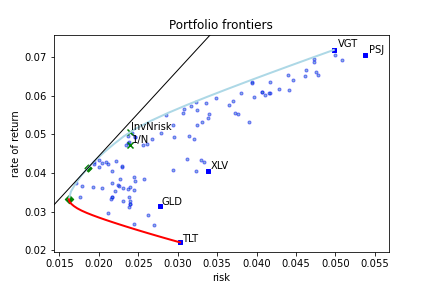
\includegraphics[width=.95\linewidth]{../figs/frontiers_1.png}
    \caption{Portfolio frontiers - expected rate of return vs. risk.}
    \label{Frontiers_1_fig}
\end{figure}

It is a generic example of portfolio frontiers. On the x-axis is the dispersion value (risk)
while on the y-axis is the expected rate of return. Given a set of financial assets, each point in this space represents a portfolio
composition. Several features are worth mentioning.


The upper blue line is the {\it efficient frontier}. This is the set of portfolios that have the highest expected rate
of return for a given risk value. These are the portfolios of interest for an investor.

The lower red line is the {\it inefficient frontier}. This is the set of portfolios that have the lowest expected rate
of return for a given risk value. Clearly, this family of portfolios are to be avoided by an investor.

The leftmost point, where the blue and red lines meet, is the {\it minimum risk portfolio}.
This is the portfolio with the smallest risk among all possible portfolios.
Investing in this class of portfolios is a relative common strategy among professional investors.

The black straight line, in the upper part of the plot, is tangent to the efficient frontier.
Its intersection with the y-axis (not shown in the plot) is at a level equal to the risk-free rate accessible to the investor.\footnote{In this example the risk-free rate was set to $0$.} The point of tangency along the efficient frontier (in our plot depicted by a green diamond)
is the so called {\it tangency portfolio} or {\it market portfolio}. This is the portfolio with the highest value of $\rho$-Sharpe ratio among all possible portfolios.
The $\rho$-Sharpe ratio is defined as
\begin{equation}
    \Sharpe = \frac{\RR-\mu_0}{\rho}, \label{ggg}
\end{equation}
where $\RR$ is the portfolio expected rate of return, $\mu_0$ is the risk-free rate accessible to the investor and
$\rho$ is the dispersion measure.\footnote{This is a generalization of the original Sharpe ratio introduced in 1966 by
William F. Sharpe \cite{Sharpe1966} as an  investment performance measure. In the original definition, $\rho$ is the
standard deviation (volatility) of the returns.}
Therefore, the portfolio that maximizes the $\rho$-Sharpe ratio is the portfolio with the highest expected excess rate of return (\ie\ above the risk-free rate) per unit of risk, $\rho$. This is a remarkable efficient portfolio often preferred by the investors.

The solid blue squares are the portfolios where the entire capital is allocated to a single component.
They are labeled by the market symbol of this portfolio component.\footnote{In our case the portfolio components are
5 ETF's: TLT, GLD, XLV, IHI and PSJ.} For short, we call them {\it single asset portfolios}.
Note that the rightmost point along the efficient frontiers is the single asset portfolio where the entire capital is invested in the portfolio component with the highest expected rate of return.
Similarly, the rightmost point along the inefficient frontier is the single asset portfolio where the entire
capital is invested in the portfolio component with the lowest expected rate of return.

All the points between the efficient (blue line) and inefficient (red line) frontiers are called {\it inefficient portfolios}.
For reference, in Fig.~\ref{Frontiers_1_fig} we depicted with small blue circles a random selection of them.
There are no valid portfolios outside the portfolio frontiers.

Among the inefficient portfolios, there is a remarkable one that has enjoined a lot of attention in the literature over the years.
This is the {\it equal weighted portfolio}.
As the name suggested, it has the weights equal to $1/N$, where $N$ is the number of portfolio components.
In Fig.~\ref{Frontiers_1_fig}, it is depicted by a green x labeled $1/N$.

On the efficient frontier, we have its correspondent. In our plot it is a green x with label InvNrisk.
This is the efficient portfolio that has the same risk as the equal weighted portfolio.

We stress that, in-sample both portfolios have the same risk while the expected rate of return is larger for InvNrisk
than for equal weighted portfolio.
However out-of-sample (especially for relatively short periods of observations) the equal weighted portfolio may outperform the InvNrisk.

\begin{figure}[H]
    \centering
    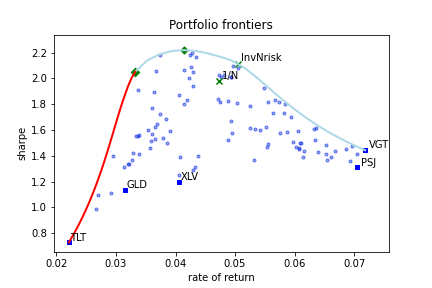
\includegraphics[width=.95\linewidth]{../figs/frontiers_2.png}
    \caption{Portfolio frontiers - $\rho$-Sharpe vs. expected rate of return.}
    \label{Frontiers_2_fig}
\end{figure}

Another way to visualize the portfolio frontiers is presented in Fig.~\ref{Frontiers_2_fig}.
It has the same information as Fig.~\ref{Frontiers_1_fig}, but now on the x-axis is the expected rate of return while on the y-axis is the $\rho$-Sharpe ratio.
We have preserved the color code and all the symbols from Fig.~\ref{Frontiers_1_fig}.
Note that in this representation the $\rho$-Sharpe portfolio is the maximum of the efficient frontier curve.

Figure~\ref{Frontiers_2_fig} gives a better understanding of portfolio efficiency in terms of expected excess return per unit of risk.

With these in mind, let's start to define the following optimization strategies. We have restricted our analysis to long-only positions in the portfolio
components.\footnote{This is a self-imposed restriction; in principle, it can be removed or replaced with specific position limits.}

\bigskip

\begin{description}
  \item[A.\label{OptRisk}]{\bf Minimization of risk for targeted expected rate of return value}

    This is the most common optimization strategy. It returns portfolio compositions along the efficient frontiers (the blue line in Figs.~\ref{Frontiers_1_fig} and
    \ref{Frontiers_2_fig}).
    Mathematically, it can be expressed as,

    \bigskip
    \noindent Minimize over $\{w_k\}_{k=1,\cdots,M}$
    \begin{subequations}\label{gg1}
    \begin{align}
        & g =  \rho\left(\sum_{k=1}^M w_k r_k \right), \label{gg1a} \\
        \st & \sum_{k=1}^M w_k \mu_k \ge \mu, \label{gg1b} \\
            & \sum_{k=1}^M w_k = 1, \label{gg1c} \\
            & w_k \ge 0. \label{gg1d}
    \end{align}
    \end{subequations}

    \noindent Here $g$ is the objective function, $\rho(\cdot)$ is the dispersion measure, $M$ is the number of portfolio component, $w_k$ are the portfolio
    weights, $r_k$ are the portfolio components rate of return
    with $\mu_k=\mE[r_k]$ their expectations and $\mu$ is the targeted portfolio expected rate of return.

    In general, if $\mu \leq \max_k\{\mu_k\}$ then the efficient portfolio expected rate of return is $\max\{\RR_{\min}, \mu \}$,
    where $\RR_{\min}$ is the minimum risk portfolio expected rate of return.
    Otherwise, the optimization problem from Eqs.~(\ref{gg1}) has no solution.

    Note that changing the direction of the inequality in Eq.~(\ref{gg1b}), the solution of the optimization problem
    will be a portfolio along the inefficient frontiers (the red line in Figs.~\ref{Frontiers_1_fig} and \ref{Frontiers_2_fig}). In this case,
    if $\mu \geq \min_k\{\mu_k\}$ then the portfolio expected rate of return is $\min\{\RR_{\min}, \mu \}$. Otherwise,
    there are no solutions.

    Equation~(\ref{gg1c}) is the weights normalization equation also called the {\it capital equation} and Eq.~(\ref{gg1d}) is the long-only positions constraint.
    These two types of equations will be present in all portfolio optimization algorithms.

  \item[B.\label{MinRisk}] {\bf Minimum risk portfolio}

    This is the efficient portfolio with the smallest risk, $\rho$.
    Mathematically, it is the solution of the above optimization problem without the constraint from Eq.~(\ref{gg1b}).

    We mentioned earlier that the optimization problem from Eqs.~(\ref{gg1}) will return the
    minimum risk portfolio if $\mu$ in Eq.~(\ref{gg1b}) is set to any value less than or equal to $\RR_{\min}$.
    In practice it is convenient to set $\mu=\min_k\{\mu_k\}$. Then, use {\it as is} the algorithm from Eqs.~(\ref{gg1}) to
    find the composition of minimum risk portfolio.
    This approach has been implemented in the \azapy\ package.

  \item[C.\label{TargetRisk}] {\bf Maximization of expected rate of return for targeted risk value}

    Another way to evaluate the efficient portfolios is to maximize the portfolio expected rate of return
    for a fixed risk vale. Mathematically this can be written as follows.

    \bigskip
    \noindent Maximize over $\{w_k\}_{j=k,\cdots,M}$
    \begin{subequations}\label{gg2}
    \begin{align}
        & g =  \sum_{k=1}^M w_k \mu_k, \label{gg2a} \\
        \st & \rho\left(\sum_{k=1}^M w_k r_k \right) = \rho_0, \label{gg2b} \\
            & \sum_{k=1}^M w_k = 1, \label{gg2c} \\
            & w_k \ge 0. \label{gg2d}
    \end{align}
    \end{subequations}

    \noindent Here $\rho_0$ is the targeted portfolio risk value.
    In general, it is unintuitive for an investor to specify outright a rational value for $\rho_0$.
    However, if $\rho_0$ is the risk value of a benchmark portfolio, then the maximization problem
    from Eqs.~(\ref{gg2}) becomes useful in computing an efficient portfolio with the same risk as the benchmark.

    An example is the efficient portfolio with the same risk as equal weighted portfolio.
    In Figs.~\ref{Frontiers_1_fig} and \ref{Frontiers_2_fig} this is the efficient portfolio depicted with green x and labeled InvNrisk.
    In general, given a dispersion measure, it is straightforward to evaluate the risk of equal weighted portfolio, $\rho_{\rm EWP}$.
    Then, the weights of InvNrisk portfolio are the solution of Eqs.~(\ref{gg2})
    for $\rho_0 = \rho_{\rm EWP}$. Given the popularity of this benchmark,
    the evaluation of InvNrisk efficient portfolio is explicitly implemented in the \azapy\ package.

  \item[D.\label{RiskAverse}] {\bf Maximization of expected rate of return for fixed risk-aversion factor}

    In this strategy the optimal portfolio weights maximize the quantity $\RR-\lambda\rho$,
    where \RR\ is the portfolio expected rate of return, $\rho$ is the dispersion measure,
    and $\lambda$ is the risk-aversion factor. $\lambda$ takes values between $0$ and $+\infty$.
    For $\lambda=0$, the optimal portfolio is the single asset portfolio where the entire capital is invested in the
    component with the highest expected rate of return.
    This is the rightmost point along the efficient frontier.
    For $\lambda=+\infty$, the optimal portfolio is the minimum risk portfolio, the leftmost point on the efficient frontier.
    Any other value for $\lambda$ will lead to an optimal portfolio along the efficient frontier.

    The maximization problem defining this strategy can be expressed as,

    \bigskip
    \noindent Maximize over $\{w_k\}_{k=1,\cdots,M}$
    \begin{subequations}\label{gg3}
    \begin{align}
        & g =  \sum_{k=1}^M w_k \mu_k - \lambda\rho\left(\sum_{k=1}^M w_k r_k \right), \label{gg3a} \\
        \st & \sum_{k=1}^M w_k = 1, \label{gg3b} \\
            & w_k \ge 0. \label{gg3c}
    \end{align}
    \end{subequations}

    \noindent It is unintuitive for an investor to specify outright a rational value for the risk-aversion factor $\lambda$.
    However, this optimization strategy may become useful if it is combined with a model to estimate the
    value of the risk-aversion factor based on the market conditions (\eg\ technical analysis, etc.).
    These risk-aversion models are beyond the scope of this paper.

    Note that the optimization problems from Eqs.~(\ref{gg1}), (\ref{gg2}) and (\ref{gg3}) are equivalent
    in the sense that they lead to the same efficient portfolios but under different parameterizations, \ie,
    \begin{quote}
    \begin{description}
        \item[$\mu$] - the expected rate of return in Eqs.~(\ref{gg1}),
        \item[$\rho_0$] - the risk targeted value in Eqs.~(\ref{gg2}),
        \item[$\lambda$] - the risk aversion factor in Eqs.~(\ref{gg3}).
    \end{description}
    \end{quote}
    From a numerical point of view, they have quite different implementations.


  \item[E.\label{MaxSharpe}] {\bf Maximization of the $\rho$-Sharpe ratio}

    Given a dispersion measure $\rho$, this is the portfolio with the highest value of $\rho$-Sharpe ratio,
    $\Sharpe$ from Eq.~(\ref{ggg}).
    It is the solution of the following optimization problem.

    \bigskip
    \noindent Maximize over $\{w_k\}_{k=1,\cdots,M}$
    \begin{subequations}\label{gg4}
    \begin{align}
        & g = \frac{ \sum_{k=1}^M w_k \mu_k - \mu_0}{\rho\left(\sum_{k=1}^M w_k r_k \right)}, \label{gg4a} \\
        \st & \sum_{k=1}^M w_k = 1, \label{gg4b} \\
            & w_k \ge 0. \label{gg4c}
    \end{align}
    \end{subequations}

    \noindent Depending on the actual mathematical structure of $\rho$, this optimization can be transformed into an
    LP, QP or SOCP problem. Formally, this procedure can be described as follows.

    {\it First step.} Introduce a new variable $t$ such that
    \begin{equation}
        \frac{1}{t} \geq \rho\left(\sum_{k=1}^M w_k r_k \right), \label{gg5}
    \end{equation}
    and the variable transformations $\bw_k = w_k t$. Then, the optimization problem from Eqs.~(\ref{gg4}) can be expressed as follows.

    \bigskip
    \noindent Maximize over $\{ \{\bw_k\}_{k=1,\cdots,M}, t\}$
    \begin{subequations}\label{gg6}
    \begin{align}
        & g =  \sum_{k=1}^M \bw_k \mu_k - \mu_0 t, \label{gg6a} \\
        \st & t\rho\left(\sum_{k=1}^M w_k r_k \right) \leq 1, \label{gg6b} \\
            & \sum_{k=1}^M \bw_k - t = 0, \label{gg6c} \\
            & \bw_k \ge 0, \label{gg6d} \\
            & t \ge 0. \label{gg6e}
    \end{align}
    \end{subequations}

    \noindent {\it Second step.} Rewrite Eq.~(\ref{gg6b}) in terms of $\{\bw_j\}_{j=1,\cdots,M}$ and $t$ as a linear or second order cone constraint.
    This will become evident in the next sections where we will deal with explicit expressions for
    $\rho$ functions.\footnote{If $\rho$ is a genuine dispersion measure (see \cite{MM}), then by definition it is positive homogeneous and
    so $t\rho\left(\sum_{k=1}^M w_k r_k \right)=\rho\left(\sum_{k=1}^M \bw_k r_k \right)$. However, writing Eq.~(\ref{gg6}) in terms of
    $\bw_k$ and $t$ only is possible for a larger class of functions $\rho$.}
    Finally, the actual weights can be recovered by dividing $\bw_j$ by $t$.

    This procedure is in the spirit of Charnes-Copper transformation \cite{Charnes} of linear fractional functional programming,
    now extended to SOCP problems.


  \item[F.\label{MinSharpe}] {\bf Minimization of the inverse $\rho$-Sharpe ratio}

    The minimization of the inverse of $\rho$-Sharpe ratio follows a similar procedure as above.
    It is described by the following optimization problem,

    \bigskip
    \noindent Minimize over $\{w_k\}_{k=1,\cdots,M}$
    \begin{subequations}\label{gg4:2}
    \begin{align}
        & g = \frac{\rho\left(\sum_{k=1}^M w_k r_k \right)}{ \sum_{k=1}^M w_k \mu_k - \mu_0}, \label{gg4a:2} \\
        \st & \sum_{k=1}^M w_k = 1, \label{gg4b:2} \\
            & w_k \ge 0. \label{gg4c:2}
    \end{align}
    \end{subequations}

    \noindent In this case the variable $t$ is defined as
    \begin{equation}
      \frac{1}{t} = \sum_{k=1}^M w_k \mu_k - \mu_0, \label{gg7}
    \end{equation}
    and the optimization problem from Eqs.~(\ref{gg4:2}) can be expressed as

    \bigskip
    \noindent Minimize over $\{\{\bw_j\}_{j=1,\cdots,M}, t\}$
    \begin{subequations}\label{gg8}
    \begin{align}
        & g = t \rho\left(\sum_{k=1}^M w_k r_k \right), \label{gg8a} \\
        \st & \sum_{k=1}^M \bw_k \mu_k - \mu_0 t = 1, \label{gg8b} \\
            & \sum_{k=1}^M \bw_k - t = 0, \label{gg8c} \\
            & \bw_k \ge 0, \label{gg8d} \\
            & t \ge 0. \label{gg8e}
    \end{align}
    \end{subequations}

    \noindent Again, the trick is to rewrite Eq.~(\ref{gg8a}) in terms of $\{\bw_k\}_{k=1,\cdots,M}$ and $t$ variables only.
    This will be made explicit in the next sections.
\end{description}

\noindent The two problems, maximization of $\rho$-Sharpe ratio and the minimization of inverse of $\rho$-Sharpe ratio, are logically
equivalent, and the solutions of Eqs.~(\ref{gg6}) and (\ref{gg8}) are the same. However, from a numerical
point of view their implementations can be quite different. In our experience both methods lead to numerical algorithms 
similar in speed and accuracy. For completeness, \azapy\ package implements both methods.


\BackToContents


\section{Tail dispersion measures}

The most famous member of this family is the Conditional Value at Risk (\CVaR).
It was introduced in 2000 as a coherent risk measure\footnote{The coherent risk measures were introduced in 1999 by
Artzner, Delbaen, Eber and Heath \cite{Artzner}.} by Rockafeller and Uryasev \cite{Uryasev} (see also \cite{Pflug}, \cite{Uryasev2}).
Since then, \CVaR\ had gained in popularity with both practitioners and financial regulators
as well as with the academic world. The literature surrounding \CVaR\ is vast and
continue to grow (see for example \cite{Mansini} and references therein).

In 2007, in an elegant paper \cite{Krokhmal}, Krokhmal introduced the Higher Moment Coherent Risk (\HMCR) measures.
Relative to the \HMCR\ family, \CVaR\ is the First Moment Coherent Risk measure.
We will follow the work of Krokhmal in introducing the main results regarding the tail dispersion measures.
The technical proofs can be found in the original paper \cite{Krokhmal}.
Later we will focus our presentation on the numerical techniques for
portfolio optimization strategies based on \CVaR\ and \SMCR\ (Second Moment Coherent Risk) dispersion measures.

For us, the key results from \cite{Krokhmal} are the following theorems.
\begin{theorem}{Krokhmal}

  \noindent Let $\Phi:\cG_T \rightarrow \mR$ be a function such that:
  \begin{enumerate}
    \item monotonicity - $\forall X\in \cG_T\ \text{with}\ X \leq 0\ \Rightarrow\ \Phi(X) \leq 0$,
    \item subadditivity - $\forall X\ \text{and}\ Y \in \cG_T,\ \Phi(X + Y) \leq \Phi(X) + \Phi(Y)$,
    \item positive homogeneity - $\forall X\in\cG_T\ \text{and}\ \lambda\in\mR^+,\ \Phi(\lambda X) = \lambda\Phi(X)$,
    \item $\forall \eta\neq 0,\ \Phi(\eta) > \eta$,
  \end{enumerate}
  then
  \begin{equation}
    \rho(X) = \min_u \left[ u + \Phi\left(-X - u\right)\right],
  \end{equation}
  exists and it is a coherent risk measure.
\end{theorem}

\begin{theorem}{Higher Momentum Coherent Risk (\HMCR) measure}

    \noindent Let $\cG_T = \cL_p(\Omega, \cF, P)$ and $\alpha \in(0,1)$ consider $\phi(X) = (1-\alpha)^{-1}\| (X)^+ \|_p$
    where $\|\cdot\|_p= \left(\mE[(|\cdot|^p)]\right)^{1/p}$. Then,
    \begin{equation}
        \HMCR_{p,\alpha}(X) = \min_u\left[u + \frac{1}{1-\alpha}\|(-X - u)^+\|_p\right],
        \label{qq0}
    \end{equation}
    is a coherent risk measure.

    \noindent The optimal value $u^*$ is called Higher Moment Value at Risk ($\HMVaR_{p,\alpha}$).
\end{theorem}

\begin{corollary}{CVaR}

    \noindent For $p=1$ we have
    \begin{equation}
        \HMCR_{1,\alpha}(X) = \min_u\left[u + \frac{1}{1-\alpha}\mE\left[ (-X - u)^+\right] \right].
        \label{qq1}
    \end{equation}
    This is the definition of \CVaR\ introduced by Rockafaller and Uryasev in \cite{Uryasev}.
    Thus, we have
    \begin{align}
        \CVaR_\alpha(X) &\equiv \HMCR_{1,\alpha}(X), \\
        \VaR_\alpha(X) &\equiv \HMVaR_{1,\alpha}(X).
    \end{align}
\end{corollary}

\begin{corollary}{SMCR}

    \noindent For $p=2$ we have
    \begin{equation}
        \HMCR_{2,\alpha}(X) = \min_u\left[u + \frac{1}{1-\alpha}\left(\mE\left[ \left(\left(-X -u\right)^+\right)^2\right]\right)^{1/2} \right].
        \label{qq2}
    \end{equation}
    Using Krokhmal terminology \cite{Krokhmal}, we call $\HMCR_{2,\alpha}(X)$ as $\SMCR_\alpha(X)$, and the optimal value $u^*$ as $\SMVaR_\alpha(X)$,
    the associated Second Moment Value at Risk  measure.
\end{corollary}

The above results were formulated in terms of risk measures in the context of risk management. It is straightforward to
export them to dispersion measures, relevant to portfolio optimizations. Since \HMCR's are coherent risk measures,
it is sufficient to replace $X$, in the r.h.s. of Eq.~(\ref{qq0}), with its detrended version $\bX = X - \mE[X]$ to
obtain a genuine dispersion measure (see \cite{MM}). From here on we refer to \HMCR\ dispersion measures.

Further, we consider the generalization to a mixture of \HMCR\ measures.
A mixture is a superposition of \HMCR's for different confidence levels, \ie,
\begin{equation}
    \mHMCR_p(X) = \sum_{l=1}^L \cK_l\times \HMCR_{p, \alpha_l}(X),
    \label{qq3}
\end{equation}
where $\{\cK_l\}_{l=1,\cdots,L}$ is a set of positive coefficients normalized to unit (the mixture coefficients) and
$\{\alpha_l\}_{l=1,\cdots,L}$ is a set of distinct confidence levels. A single \HMCR\ is a special case of \mHMCR\ for $L=1$ in Eq.~(\ref{qq3}).

The next two subsections present the optimal portfolio strategies based on $\mHMCR_p$ for $p=1$ and $p=2$, respectively, \ie,
\begin{align}
    \mCVaR(X) &\equiv \mHMCR_1(X), \label{qq4} \\
    \mSMCR(X) &\equiv \mHMCR_2(X). \label{qq5}
\end{align}


\BackToContents


\subsection{mCVaR-based optimization strategies}\label{S:mCVaR}

This section presents portfolio optimization strategies based on the mixture \CVaR\ dispersion measure, \ie,
\begin{equation}
    \mCVaR = \sum_{l=1}^{L} \cK_l \times \CVaR_{\alpha_l},
    \label{cvar0}
\end{equation}
where $\{\cK_l\}_{l=1,\cdots,L}$ is a set of positive coefficients normalized to unit (the mixture coefficients),
$\{\alpha_l\}_{l=1,\cdots,L}$ is a set of distinct confidence levels and
\begin{equation}
    \CVaR_\alpha(X) = \min_u\left[u + \frac{1}{1-\alpha}\mE\left[(-\bX-u)^+\right] \right],
    \label{cvarS}
\end{equation}
where $\bX = X - \mE[X]$.

On the side note, \mCVaR\ can be viewed as a particular case of
a Spectral measure \cite{Acerbi}.

\BackToContents


\subsubsection{mCVaR dispersion measure}

We start by listing the main result from Rockafaller and Uryasev \cite{Uryasev}.
Given a set of observed rates of returns, $\{r_i\}_{i=1,\cdots,N}$,
the \CVaR\ from Eq.~(\ref{cvarS}) can be rewritten as
\begin{equation}
    \CVaR_\alpha = \min_u\left[ u +  \frac{1}{(1-\alpha)N} \sum_{i=1}^N \left(-u -\br_i \right)^+ \right],
    \label{cvar1:1}
\end{equation}
where $\br_i = r_i - \frac{1}{N}\sum_{j=1}^N r_j$ are the detrended historical observations and
$\alpha$ is the confidence level.\footnote{A typical value could be 0.975, then \CVaR\ is the
average return of the 2.5 percentile.}


It is straightforward to show that, Eq~(\ref{cvar1:1}) can be transformed into the
following LP problem.

\bigskip
\noindent Minimize over $\{u, \{s_i\}_{i=1,\cdots,N}\}$
\begin{subequations}\label{cvar1}
\begin{align}
    &g = u + \frac{1}{(1-\alpha) N} \sum_{i=1}^N s_i, \label{cvar1a} \\
    \st & s_i + u \geq - \br_i, \label{cvar1b} \\
        & s_i \geq 0, \label{cvar1c} \\
        & u \geq 0. \label{cvar1d}
\end{align}
\end{subequations}

\noindent Then, we have
\begin{subequations}\label{cvar2}
\begin{align}
    \CVaR_\alpha &= g^*, \label{cvar2a} \\
    \VaR_\alpha &= u^*, \label{cvar2b}
\end{align}
\end{subequations}

\noindent where $^*$ denotes the solution of LP problem.


The LP problem from Eqs.~(\ref{cvar1}) has an analytical solution. It can be described as follows.

\bigskip
\noindent Let $\{x_i\}_{i=1,\cdot,N}$
be $\{\br_i\}_{i=1,\cdot,N}$ sorted in ascending order. Then, we have
\begin{subequations}\label{cvar3}
\begin{align}
    \CVaR &= \frac{k^* - a}{a} x_{k^*} - \frac{1}{a} \sum_{i=1}^{k^*} x_i, \label{cvar3a} \\
    \VaR &= x_{k^*}, \label{cvar3b}
\end{align}
\end{subequations}
where
\begin{subequations}\label{cvar4}
\begin{align}
    a &= N(1-\alpha), \label{cvar4a} \\
    k^* &= \lceil a \rceil. \label{cvar4b}
\end{align}
\end{subequations}

\noindent Here $\lceil\cdot\rceil$ denotes the ceiling operator.
A sketched proof of this result is in Appendix~\ref{AppendixA}.

\noindent Further, \mCVaR\ is given by the sum from Eq.~(\ref{cvar0}).

Form a numerical point of view, the implementation of the analytic solution is preferred over the LP algorithm.
This approach has been implemented in the \azapy\ package.
However, the transformation of Eq.~(\ref{cvar1:1})
into the LP problem from Eqs.~(\ref{cvar1}) is at the core of all LP formulations for \mCVaR-based optimal portfolio strategies.
There are no analytical solutions for these LP problems.
Therefore, the numerical algorithms for optimizations must involve LP solvers.

\BackToContents

\subsubsection{mCVaR optimal portfolio}

Formally, this optimization is described by Eqs.~(\ref{gg1}) from Sec.~\ref{strategies} point~\ref{OptRisk},
where $\rho$ is given by the \mCVaR\ from Eq.\ (\ref{cvar0}).
It is straightforward to show that, this optimization is given by the following LP problem.

\bigskip
\noindent Minimize over $\{\{w_k\}_{k=1,\cdots,M}, \{ u_l, \{s_{li}\}_{i=1,\cdots,N}\}_{l=1,\cdots,L}\}$
\begin{subequations}\label{cvar5}
\begin{align}
    &g = \sum_{l=1}^{L}\cK_l \left( u_l + \frac{1}{(1-\alpha_l)N} \sum_{i=1}^N s_{li} \right), \label{cvar5a} \\
    \st &s_{li} + u_l + \sum_{k=1}^M w_k \br_{ki} \geq 0, \label{cvar5b} \\
        &\sum_{k=1}^M w_k \mu_k \geq \mu, \label{cvar5c} \\
        &\sum_{k=1}^M w_k = 1, \label{cvar5d} \\
        & s_{li} \geq 0, \label{cvar5e} \\
        & u_l \geq 0, \label{cvar5f} \\
        & w_k \geq 0, \label{cvar5g}
\end{align}
\end{subequations}

\noindent where $\mu$ from Eq.~(\ref{cvar5c}) is the portfolio targeted expected rate of return, while $\{\mu_k\}_{k = 1,\cdots,M}$
are the portfolio components expected rate of return. Here, $\br_{ki}$ is the $i$-th detrended\footnote{After
the subtraction of their average, \ie\ $\br_{ki} = r_{ki} - \frac{1}{N}\sum_{j=1}^N r_{kj}$.} observation of the
$k$-th portfolio component rate of return.
Then, we have
\begin{subequations}\label{cvar6}
\begin{align}
    \mCVaR &= g^*, \label{cvar6a} \\
    \RR &= \sum_{k=1}^M w_k^* \mu_k, \label{cvar6b} \\
    \CVaR_{\alpha_l} &= u_l^* + \frac{1}{(1-\alpha_l)N} \sum_{i=1}^N s_{li}^*, \label{cvar6c} \\
    \VaR_{\alpha_l} &= u_l^*, \label{cvar6d}
\end{align}
\end{subequations}

\noindent where the $^*$ denotes the solution of LP problem.
In addition to the optimal portfolio weights $\{w_k^*\}_{k=1,\cdots,M}$
and the portfolio expected rate of return $\RR$,
the LP solution provides information about the portfolio \mCVaR\ and its  \CVaR\
and associated \VaR\ components.


\bigskip
\noindent Here is an example, using the \azapy\ package, of how to compute the \mCVaR\ optimal portfolio.
The \mCVaR\ time horizon was set to one quarter and the calibration is performed using the prior 3.25 years of
close-adjusted historical prices (default settings).
For more details see the package documentation at \azapydoc.

\lstinputlisting[language=Python]{../PyScripts/CVaR_RiskOptim.py}

\BackToContents

\subsubsection{Minimum mCVaR portfolio}

Following the results from Sec.~\ref{strategies} point~\ref{MinRisk},
the algorithm to compute the optimal portfolio with minimum \mCVaR\ is given by the LP problem from Eqs.~(\ref{cvar5}) where
$\mu$ from r.h.s. of Eq.~(\ref{cvar5c}) is set to a value equal to the smallest expected rate of
return among the portfolio components, \ie\ $\mu = \min_k\{\mu_k\}$.

\bigskip
\noindent Here is an example, using the \azapy\ package, of how to compute the minimum \mCVaR\ portfolio.
The \mCVaR\ time horizon was set to one quarter and the calibration is performed using the prior 3.25 years of
close-adjusted historical prices (default settings).
For more details see the package documentation at \azapydoc.

\lstinputlisting[language=Python]{../PyScripts/CVaR_MinRisk.py}

\BackToContents

\subsubsection{mCVaR optimal portfolio for targeted risk value}

This optimization is described by Eqs.~(\ref{gg2}) from Sec.~\ref{strategies} point~\ref{TargetRisk},
where $\rho$ is given by the \mCVaR\ from Eq.~(\ref{cvar0}).
It is the following LP problem.

\bigskip
\noindent Maximize over $\{ \{w_k\}_{k=1,\cdots,M}, \{ u_l, \{ s_{li}\}_{i=1,\cdots,N} \}_{l=1,\cdots, L}\}$
\begin{subequations}\label{cvar7}
\begin{align}
    &g = \sum_{k=1}^M w_k \mu_k, \label{cvar7a} \\
    \st & \sum_{l=1}^L \cK_l \left( u_l + \frac{1}{(1-\alpha_l) N} \sum_{i=1}^N s_{li} \right) = \mCVaR_0, \label{cvar7c} \\
        &s_{li} + u_l + \sum_{k=1}^M w_k \br_{ki} \geq 0, \label{cvar7b} \\
        & \sum_{k=1}^M w_k = 1, \label{cvar7d} \\
        & s_{li} \geq 0, \label{cvar7e} \\
        & u_l \geq 0, \label{cvar7f} \\
        & w_k \geq 0, \label{cvar7g}
\end{align}
\end{subequations}

\noindent where $\mCVaR_0$ in Eq.~(\ref{cvar7c}) is the portfolio targeted \mCVaR\ dispersion value.
Then, we have
\begin{subequations}\label{cvar8}
\begin{align}
    \RR &= g^*, \label{cvar8a} \\
    \CVaR_{\alpha_l} &= u_l^* + \frac{1}{(1-\alpha_l) N}\sum_{i=1}^N s_{li}^*, \label{cavr8b} \\
    \VaR_{\alpha_l} &= u_l^*, \label{cvar8c}
\end{align}
\end{subequations}

\noindent where $^*$ denotes the solution of LP problem.
In addition to the optimal portfolio weights $\{w_k^*\}_{k=1,\cdots,M}$ and the portfolio expected rate of return $\RR$,
the LP solution provides information about the \CVaR\ and associated \VaR\ components of $\mCVaR_0$,
although, this information is likely to be known at the outset.

\bigskip
\noindent Here is an example, using the \azapy\ package, of how to compute the optimal portfolio
with the same \mCVaR\ as the equal weighted portfolio.
The \mCVaR\ time horizon was set to one quarter and the calibration is performed using the prior 3.25 years of
close-adjusted historical prices (default settings).
For more details see the package documentation at \azapydoc.

\lstinputlisting[language=Python]{../PyScripts/CVaR_InvNrisk.py}

\BackToContents

\subsubsection{mCVaR optimal portfolio for fixed risk-aversion factor}
This optimization is described by Eqs.~(\ref{gg3}) from Sec.~\ref{strategies} point~\ref{RiskAverse},
where $\rho$ is given by \mCVaR\ from Eq.~(\ref{cvar0}).
It is the following LP problem.

\bigskip
\noindent Maximize over $\{\{w_k\}_{k=1,\cdots,M}, \{ u_l, \{s_{li}\}_{i=1,\cdots,N}\}_{l=1,\cdots,L}\}$
\begin{subequations}\label{cvar9}
\begin{align}
    &g = \sum_{k=1}^M w_k \mu_k - \lambda \sum_{l=1}^{L}\cK_l \left( u_l + \frac{1}{(1-\alpha_l)N} \sum_{i=1}^N s_{li} \right), \label{cvar9a} \\
    \st &s_{li} + u_l + \sum_{k=1}^M w_k \br_{ki} \geq 0, \label{cvar9b} \\
        &\sum_{k=1}^M w_k = 1, \label{cvar9c} \\
        & s_{li} \geq 0, \label{cvar9d} \\
        & u_l \geq 0, \label{cvar9e} \\
        & w_k \geq 0, \label{cvar9f}
\end{align}
\end{subequations}

\noindent where $\lambda$ from Eqs.~(\ref{cvar9a}) is the risk-aversion factor.
Then, we have
\begin{subequations}\label{cvar10}
\begin{align}
    \RR &= \sum_{k=1}^M w_k^* \mu_k, \label{cvar10a} \\
    \mCVaR &= \frac{\RR - g^*}{\lambda}, \label{cvar10b} \\
    \CVaR_{\alpha_l} &= u_l^* + \frac{1}{(1-\alpha_l)N} \sum_{i=1}^N s_{li}^*, \label{cvar10c} \\
    \VaR_{\alpha_l} &= u_l^*, \label{cvar10d}
\end{align}
\end{subequations}

\noindent where $^*$ denotes the solution of LP problem.
In addition to the optimal portfolio weights $\{w_k^*\}_{k=1,\cdots,M}$ and the portfolio expected rate of return $\RR$,
the LP solution provides information about the portfolio \mCVaR\ and its \CVaR\  and associated \VaR\ components.

\bigskip
\noindent Here is an example, using the \azapy\ package, of how to compute the optimal portfolio
for a given value of the risk-aversion factor $\lambda$.
The \mCVaR\ time horizon was set to one quarter and the calibration is performed using the prior 3.25 years of
close-adjusted historical prices (default settings).
For more details see the package documentation at \azapydoc.

\lstinputlisting[language=Python]{../PyScripts/CVaR_Averse.py}

\BackToContents

\subsubsection{mCVaR-Sharpe optimal portfolio - maximization solution}
This optimization targets the maximization of \mCVaR-Sharpe
ratio.\footnote{\mCVaR-Sharpe ratio is defined by Eq.~(\ref{ggg}) where $\rho=\mCVaR$.}
It is based on the Eqs.~(\ref{gg4}) from Sec.~\ref{strategies} point~\ref{MaxSharpe},
where $\rho$ is given by the \mCVaR\ from Eq.~(\ref{cvar0}).
The optimization can be formulated as an LP problem if Eq.~(\ref{gg4b}) can be linearized.
In our case the linearization is straightforward. Introducing the
variable transformations $\bw_k = t w_k$, $\bs_{li} = t s_{li}$ and $\bu_l = t u_l$, the LP
problem can be written as follows.

\bigskip
\noindent Maximize over $\{\{\bw_k\}_{k=1,\cdots,M}, \{ \bu_l, \{\bs_{li}\}_{i=1,\cdots,N}\}_{l=1,\cdots,L}, t\}$
\begin{subequations}\label{cvar11}
\begin{align}
    &g = \sum_{i=1}^M \bw_k \mu_k - \mu_0 t, \label{cvar11a} \\
    \st &\sum_{l=1}^L \cK_l \left( \bu_l + \frac{1}{(1 - \alpha_l) N} \sum_{i=1}^N \bs_{li} \right) = 1, \label{cvar11d} \\
        &\bs_{li} + \bu_l + \sum_{k=1}^M \bw_k \br_{ki} \geq 0, \label{cvar11b} \\
        &\sum_{k=1}^M \bw_k - t = 0, \label{cvar11c} \\
        &t \geq 0, \label{cvar11h} \\
        &\bs_{li} \geq 0, \label{cvar11e} \\
        &\bu_l \geq 0, \label{cvar11f} \\
        &\bw_k \geq 0, \label{cvar11g}
\end{align}
\end{subequations}

\noindent where $\mu_0$ from Eq.~(\ref{cvar11a}) is the risk-free rate accessible to the investor.
Then, we have
\begin{subequations}\label{cvar12}
\begin{align}
    w_k &= \frac{\bw_k^*}{t^*} , \label{cvar12a} \\
    \RR &= \frac{g^*}{t^*}  + \mu_0, \label{cvar12b} \\
    \Sharpe & = g^*, \label{cvar12c} \\
    \mCVaR &= \frac{1}{t^*}, \label{cvar12d} \\
    \CVaR_{\alpha_l} &= \frac{1}{t^*} \left( \bu_l^* + \frac{1}{(1 - \alpha_l) N} \sum_{i=1}^N \bs_{li}^* \right), \label{cvar12e} \\
    \VaR_{\alpha_l} &= \frac{\bu_l^*}{t^*} , \label{cvar12f}
\end{align}
\end{subequations}

\noindent where $^*$ denotes the solution of LP problem.
In addition to the optimal portfolio weights $\{w_k\}_{k=1,\cdots,M}$, expected rate of return $\RR$ and \mCVaR-Sharpe ratio $\Sharpe$,
the LP solution provides information about the portfolio \mCVaR\ and its \CVaR\  and associated \VaR\ components.

\bigskip
\noindent Here is an example, using the \azapy\ package, of how to compute the \mCVaR-Sharpe optimal portfolio using the maximization
of \mCVaR-Sharpe ratio.
The \mCVaR\ time horizon was set to one quarter and the calibration is performed using the prior 3.25 years of
close-adjusted historical prices (default settings).
For more details see the package documentation at \azapydoc.

\lstinputlisting[language=Python]{../PyScripts/CVaR_Sharpe.py}

\BackToContents

\subsubsection{mCVaR-Sharpe optimal portfolio - minimization solution}
This optimization targets the minimization of the inverse of \mCVaR-Sharpe ratio.
It is  described by Eqs.~(\ref{gg8}) from Sec.~\ref{strategies} point~\ref{MinSharpe}, where
$\rho$ is given by \mCVaR\ from Eq.~(\ref{cvar0}).
The optimization can be formulated as an LP problem if Eq.~(\ref{gg8a}) can be linearized. This can be achieved by
introducing the following variable transformations
$\bw_k = t w_k$, $\bs_{li} = t s_{li}$ and $\bu_l = t u_l$.
Then, the LP problem can be written as follows.

\bigskip
\noindent Minimize over $\{\{\bw_k\}_{k=1,\cdots,M}, \{ \bu_l, \{\bs_{li}\}_{i=1,\cdots,N}\}_{l=1,\cdots,L}, t\}$
\begin{subequations}\label{cvar13}
\begin{align}
    &g = \sum_{l=1}^L \cK_l \left( \bu_l + \frac{1}{(1 - \alpha_l) N} \sum_{i=1}^N \bs_{li} \right), \label{cvar13a} \\
    \st &\sum_{k=1}^M \bw_k \mu_k - t\mu_0 = 1, \label{cvar13c} \\
        &\bs_{li} + \bu_l + \sum_{k=1}^M \bw_k \br_{ki} \geq 0, \label{cvar13b} \\
        &\sum_{k=1}^M \bw_k - t = 0, \label{cvar13d} \\
        &t \geq 0, \label{cvar13h} \\
        &\bs_{li} \geq 0, \label{cvar13e} \\
        &\bu_l \geq 0, \label{cvar13f} \\
        &\bw_k \geq 0, \label{cvar13g}
\end{align}
\end{subequations}

\noindent where $\mu_0$ from Eq.~(\ref{cvar13c}) is the risk-free rate accessible to the investor.
Then, we have
\begin{subequations}\label{cvar14}
\begin{align}
    w_k &= \frac{\bw_k^*}{t^*} , \label{cvar14a} \\
    \RR &= \frac{1}{t^*} + \mu_0, \label{cvar14b} \\
    \Sharpe &= \frac{1}{g^*}, \label{cvar14c} \\
    \mCVaR &= \frac{g^*}{t^*} , \label{cvar14d} \\
    \CVaR_{\alpha_l} &= \frac{1}{t^*} \left( \bu_l^* + \frac{1}{(1 - \alpha_l) N} \sum_{i=1}^N \bs_{li}^* \right), \label{cvar14e} \\
    \VaR_{\alpha_l} &= \frac{\bu_l^*}{t^*} , \label{cvar14f}
\end{align}
\end{subequations}

\noindent where $^*$ denotes the solution of LP problem.
In addition to the optimal portfolio weights $\{w_k\}_{k=1,\cdots,M}$, expected rate of return $\RR$ and \mCVaR-Sharpe ratio $\Sharpe$,
the LP solution provides information about the portfolio \mCVaR\ and its \CVaR\  and associated \VaR\ components.

\bigskip
\noindent Here is an example, using the \azapy\ package, of how to compute the \mCVaR-Sharpe optimal portfolio using the minimization
of the inverse of \mCVaR-Sharpe ratio.
The \mCVaR\ time horizon was set to one quarter and the calibration is performed using the prior 3.25 years of
close-adjusted historical prices (default settings).
For more details see the package documentation at \azapydoc.

\lstinputlisting[language=Python]{../PyScripts/CVaR_InvSharpe.py}

\BackToContents

\subsubsection{mCVaR frontiers}

Here is an example of how to compute the \mCVaR\ frontiers using the \azapy\
package. The \mCVaR\ time horizon was set to one quarter and the calibration is performed using the prior 3.25 years of
close-adjusted historical prices (default settings).
For more details see the package documentation at \azapydoc.

The script produces the plots in Figs.~\ref{CVaR_fig1a} and \ref{CVaR_fig1b}
for historical data collected up to 2021-07-27.

\lstinputlisting[language=Python]{../PyScripts/CVaR_frontiers.py}

\begin{figure}[H]
\centering
\begin{subfigure}{.5\textwidth}
  \centering
  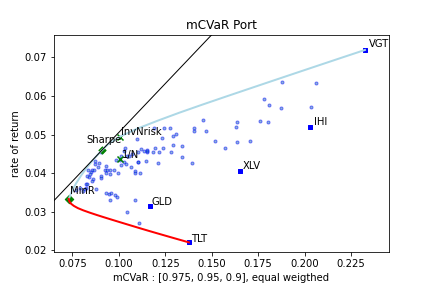
\includegraphics[width=.95\linewidth]{../figs/mCVaRFrontier1.png}
  \caption{Rate of return vs. \mCVaR}
  \label{CVaR_fig1a}
\end{subfigure}%
\begin{subfigure}{.5\textwidth}
  \centering
  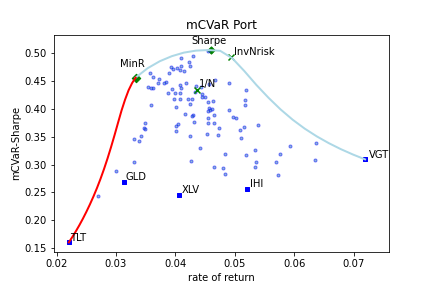
\includegraphics[width=.95\linewidth]{../figs/mCVaRFrontier2.png}
  \caption{\mCVaR-Sharpe vs. rate of return}
  \label{CVaR_fig1b}
\end{subfigure}
\caption{\mCVaR\ : [$\alpha=(0.975, 0.95, 0.9)$, equal weighted] frontiers.}
\label{CVaR_fig1}
\end{figure}

\BackToContents

\subsubsection{Backtesting mCVaR-Sharpe optimal portfolio}

Here is an example, using \azapy\ package, of computing a portfolio backtesting.
For this example, we have chosen a portfolio quarterly rebalanced according
to the maximization of \mCVaR-Sharpe ratio. At each rebalancing date,
the portfolio weights
are calibrated based on 3.25 years of prior historical market data (default settings).

Other rebalancing strategies can be considered
by changing the value of {\it rtype} parameter in the call of {\it set\_model} function below.
For more details see the package documentation at \azapydoc.

\lstinputlisting[language=Python]{../PyScripts/CVaR_Port.py}

\begin{figure}[H]
    \centering
    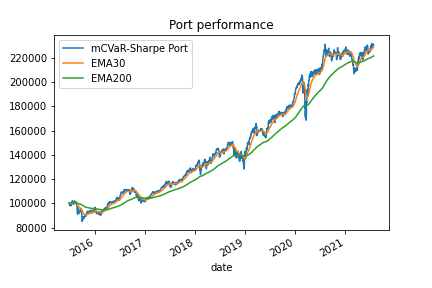
\includegraphics[width=.95\linewidth]{../figs/Port_mCVaR_Sharpe.png}
    \caption{Backtesting of quarterly rebalanced \mCVaR-Sharpe optimal portfolio,
    \mCVaR\ : [$\alpha=(0.975, 0.95, 0.9)$, equal weighted].}
    \label{CVaR_Port_fig}
\end{figure}

\BackToContents 

\subsection{mSMCR-based optimization strategies}\label{S:mSMCR}

This section presents portfolio optimization strategies based on the
mSMCR dispersion measure, \ie,
\begin{equation}
    \mSMCR = \sum_{l=1}^L \cK_l \times \SMCR_{\alpha_l},
    \label{smcr0}
\end{equation}
where $\{\cK_l\}_{l=1,\cdots,L}$ is a set of positive coefficients normalized to unit (the mixture coefficients),
$\{\alpha_l\}_{l=1,\cdots,L}$ is a set of distinct confidence levels  and
\begin{equation}
    \SMCR_\alpha(r) = \min_u\left( u + \frac{1}{1-\alpha} \left\| (-\br -u)^+ \right\|_2 \right),
    \label{smcrS}
\end{equation}
where $\br = r - \mE[r]$ is the detrended rate of return and $\|\cdot\|_2 = (\mE[|\cdot|^2])^{1/2}$ is the $L^2$-norm.

\BackToContents


\subsubsection{mSMCR dispersion measure}

This subsection presents the SOCP approximation for \mSMCR\ dispersion measure.

Given a set $\{r_i\}_{i=1,\cdots,N}$ of observed rates of return, Eq.~(\ref{smcrS}) can be rewritten as
\begin{equation}
    \SMCR_\alpha = \min_u\left[ u + \frac{1}{(1-\alpha)\sqrt{N}}\left( \sum_{i=1}^N \left[(-u - \br_i)^+\right]^2 \right)^{1/2} \right].
    \label{smcr1:1}
\end{equation}
It is straightforward to show that, Eq.~(\ref{smcr1:1}) can be transformed into the following SOCP problem,

\bigskip
\noindent Minimize over $\{u, \eta, \{s_i\}_{i=1,\cdots,N}\}$
\begin{subequations}\label{smcr1}
\begin{align}
    &g = u + \frac{\eta}{1-\alpha} , \label{smcr1a} \\
    \st &\left( \frac{1}{N}\sum_{i=1}^N s_i^2 \right)^{1/2} \leq \eta, \label{smcr1b} \\
        &s_i + u \geq -\br_i, \label{smcr1c} \\
        &s_i \geq 0, \label{smcr1d} \\
        &\eta \geq 0, \label{smcr1e} \\
        &u \geq 0, \label{smcr1f}
\end{align}
\end{subequations}

\noindent where $\br_i$ is the i-th detrended rate of return, \ie\ $\br_i = r_i - \frac{1}{N}\sum_{j=1}^N r_j$.
Then, we have
\begin{subequations}\label{smcr2}
\begin{align}
    \SMCR_\alpha &= g^*, \label{smcr2a} \\
    \SMVaR_\alpha & = u^*, \label{smcr2b}
\end{align}
\end{subequations}

\noindent where $^*$ denotes the solutions of SOCP problem.

Further, \mSMCR\ is given by the sum from Eq.~(\ref{smcr0}).
In total there are $L$ decoupled SOCP problems, one for each mixture element.

Note that, the transformation of Eq.~(\ref{smcr1:1}) into the SOCP problem from Eqs.~(\ref{smcr1})
is at the core of all \mSMCR-based optimal portfolio algorithms. However, in these cases all the mixture elements
will be coupled in a single SOCP problem.

\BackToContents

\subsubsection{mSMCR optimal portfolio}
The optimization is described by Eqs.~(\ref{gg1}) from Sec.~\ref{strategies} point~\ref{OptRisk},
where $\rho$ is given by \mSMCR\ from Eq.~(\ref{smcr0}).
It is the following SOCP problem.

\bigskip
\noindent Minimize over $\{ \{w_k\}_{k=1,\cdots,M}, \{ u_l, \eta_l, \{s_{li}\}_{i=1,\cdots,N} \}_{l=1,\cdots,L}\}$
\begin{subequations}\label{smcr3}
\begin{align}
    &g = \sum_{l=1}^L \cK_l \left( u_l + \frac{\eta_l}{1 - \alpha_l}  \right), \label{smcr3a} \\
    \st &\left( \frac{1}{N}  \sum_{i=1}^N s_{li}^2 \right)^{1/2} \leq \eta_l, \label{smcr3b} \\
        &s_{li} + u_l + \sum_{k=1}^M w_k \br_{ki} \geq 0, \label{smcr3c} \\
        &\sum_{k=1}^M w_k \mu_k \geq \mu, \label{smcr3d} \\
        &\sum_{k=1}^M w_k = 1, \label{smcr3e} \\
        &s_{li} \geq 0, \label{smcr3f} \\
        &\eta_l \geq 0, \label{smcr3h} \\
        &u_l \geq 0, \label{smcr3i} \\
        &w_k \geq 0, \label{smcr3g}
\end{align}
\end{subequations}

\noindent where $\mu$ in Eq.~(\ref{smcr3d}) is the portfolio targeted expected rate of return, $\mu_k$ for $k=1,\cdots,M$
are the portfolio components expected rate of returns and $\br_{ki}$ in Eq.~(\ref{smcr3c}) is the $i$-th detrended observation of the
$k$-th portfolio component rate of return.
Then, we have
\begin{subequations}\label{smcr4}
\begin{align}
    \RR &= \sum_{k=1}^M w_k^* \mu_k, \label{smcr4a} \\
    \mSMCR &= g^*, \label{smcr4b} \\
    \SMCR_{\alpha_l} &= u_l^* + \frac{\eta_l^*}{1-\alpha_l} , \label{smcr4c} \\
    \SMVaR_{\alpha_l} &= u_l^*, \label{smcr4d}
\end{align}
\end{subequations}

\noindent where $^*$ denotes the solution of SOCP problem.
In addition to the optimal portfolio weights $\{w_k^*\}_{k=1,\cdots,M}$ and the expected rate of return $\RR$,
the SOCP solution provides information about the portfolio \mSMCR\ and its \SMCR\  and
associated \SMVaR\ components.

\bigskip
\noindent Here is an example, using the \azapy\ package, of how to compute the \mSMCR\ optimal portfolio.
The \mSMCR\ time horizon was set to one quarter and the calibration is performed using the prior 3.25 years of
close-adjusted historical prices (default settings).
For more details see the package documentation at \azapydoc.

\lstinputlisting[language=Python]{../PyScripts/SMCR_RiskOptim.py}

\BackToContents

\subsubsection{Minimum mSMCR portfolio}
Following the results from Sec.~\ref{strategies} point~\ref{MinRisk},
the algorithm to compute the optimal portfolio with minimum \mSMCR\ is given by the SOCP problem from Eqs.~(\ref{smcr3}) where
$\mu$ from r.h.s. of Eq.~(\ref{smcr3d}) is set to a value equal to the smallest expected rate of
return among the portfolio components, \ie\ $\mu = \min_k\{\mu_k\}$.

\bigskip
\noindent Here is an example, using the \azapy\ package, of how to compute the minimum \mSMCR\ portfolio.
The \mSMCR\ time horizon was set to one quarter and the calibration is performed using the prior 3.25 years of
close-adjusted historical prices (default settings).
For more details see the package documentation at \azapydoc.

\lstinputlisting[language=Python]{../PyScripts/SMCR_MinRisk.py}

\BackToContents

\subsubsection{mSMCR optimal portfolio for targeted risk value}
The optimization is described by Eqs.~(\ref{gg2}) from Sec.~\ref{strategies} point~\ref{TargetRisk}, where
$\rho$ is given by \mSMCR\ from Eq.~(\ref{smcr0}).
It is the following SOCP problem.

\bigskip
\noindent Maximize over $\{ \{w_k\}_{k=1,\cdots,M}, \{ u_l, \eta_l, \{ s_{li}\}_{i=1,\cdots,N} \}_{l=1,\cdots, L}\}$
\begin{subequations}\label{smcr5}
\begin{align}
    &g = \sum_{k=1}^M w_k \mu_k, \label{smcr5a} \\
    \st &\left( \frac{1}{N} \sum_{i=1}^N s_{li}^2 \right)^{1/2} \leq \eta_l, \label{smcr5b} \\
        &s_{li} + u_l + \sum_{k=1}^M w_k \br_{ki} \geq 0, \label{smcr5c} \\
        &\sum_{l=1}^L \cK_l\left( u_l + \frac{\eta_l}{1 - \alpha_l} \right) = \mSMCR_0, \label{smcr5d} \\
        &\sum_{k=1}^M w_k = 1, \label{smcr5e} \\
        &s_{li} \geq 0, \label{smcr5f} \\
        &\eta_l \geq 0, \label{smcr5h} \\
        &u_l \geq 0, \label{smcr5i} \\
        &w_k \geq 0, \label{smcr5g}
\end{align}
\end{subequations}

\noindent where $\mSMCR_0$ in Eq.~(\ref{smcr5d}) is the portfolio targeted \mSMCR\ dispersion value.
Then, we have
\begin{subequations}\label{smcr6}
\begin{align}
    \RR &= g^*, \label{smcr6a} \\
    \SMCR_{\alpha_l} &= u_l^* + \frac{\eta_l^*}{1-\alpha_l} , \label{smcr6b} \\
    \SMVaR_{\alpha_l} &= u_l^*, \label{smcr6c}
\end{align}
\end{subequations}

\noindent where $^*$ denotes the solution of SOCP problem.
In addition to the optimal portfolio weights $\{w_k^*\}_{k=1,\cdots,M}$ and the portfolio expected rate of return $\RR$,
the SOCP solution provides information about the value of the \SMCR\ and associated \SMVaR\
components of $\mSMCR_0$, although, this information is likely to be known at the outset.

\bigskip
\noindent Here is an example, using the \azapy\ package, of how to compute the optimal portfolio
with the same \mSMCR\ as the equal weighted portfolio.
The \mSMCR\ time horizon was set to one quarter and the calibration is performed using the prior 3.25 years of
close-adjusted historical prices (default settings).
For more details see the package documentation at \azapydoc.

\lstinputlisting[language=Python]{../PyScripts/SMCR_InvNrisk.py}

\BackToContents

\subsubsection{mSMCR optimal portfolio for fixed risk-aversion factor}
The optimization is described by Eqs.~(\ref{gg3}) from Sec.~\ref{strategies} point~\ref{RiskAverse},
where $\rho$ is given by \mSMCR\ from Eq.~(\ref{smcr0}).
It is the following SOCP problem.

\bigskip
\noindent Maximize over $\{ \{w_k\}_{k=1,\cdots,M}, \{ u_l, \eta_l, \{s_{li}\}_{i=1,\cdots,N} \}_{l=1,\cdots,L}\}$
\begin{subequations}\label{smcr7}
\begin{align}
    &g = \sum_{k=1}^M w_k\mu_k - \lambda \sum_{l=1}^L \cK_l \left( u_l + \frac{\eta_l}{1 - \alpha_l}  \right), \label{smcr7a} \\
    \st &\left( \frac{1}{N} \sum_{i=1}^N s_{li}^2 \right)^{1/2} \leq \eta_l, \label{smcr7b} \\
        &s_{li} + u_l + \sum_{k=1}^M w_k \br_{ki} \geq 0, \label{smcr7c} \\\
        &\sum_{k=1}^M w_k = 1, \label{smcr7d} \\
        &s_{li} \geq 0, \label{smcr7e} \\
        &\eta_l \geq 0, \label{smcr7g} \\
        &u_l \geq 0, \label{smcr7h} \\
        &w_k \geq 0, \label{smcr7f}
\end{align}
\end{subequations}

\noindent where $\lambda$ from Eqs.~(\ref{smcr7a}) is the risk-aversion factor.
Then, we have
\begin{subequations}\label{smcr8}
\begin{align}
    \RR &= \sum_{k=1}^M w_k^* \mu_k, \label{smcr8a} \\
    \mSMCR &= \frac{\RR - g^*}{\lambda}, \label{smcr8b} \\
    \SMCR_{\alpha_l} &= u_l^* + \frac{\eta_l^*}{1-\alpha_l} , \label{smcr8c} \\
    \SMVaR_{\alpha_l} &= u_l^*, \label{smcr8d}
\end{align}
\end{subequations}

\noindent where $^*$ denotes the solution of SOCP problem.
In addition to the portfolio weights $\{w_k^*\}_{k=1,\cdots,M}$ and the portfolio expected rate of return $\RR$,
the SOCP solution provides information about portfolio $\mSMCR$ and its \SMCR\  and
associated \SMVaR\ components.

\bigskip
\noindent Here is an example, using the \azapy\ package, of how to compute the optimal portfolio
for a given value of the risk-aversion factor $\lambda$.
The \mSMCR\ time horizon was set to one quarter and the calibration is performed using the prior 3.25 years of
close-adjusted historical prices (default settings).
For more details see the package documentation at \azapydoc.

\lstinputlisting[language=Python]{../PyScripts/SMCR_Averse.py}

\BackToContents

\subsubsection{mSMCR-Sharpe optimal portfolio - maximization solution}
This optimization targets the maximization of \mSMCR-Sharpe ratio.
It is described by Eqs.~(\ref{gg4}) from Sec.~\ref{strategies} point~\ref{MaxSharpe},
where $\rho$ is given by \mSMCR\ from Eq.~(\ref{smcr0}).
The optimization can be formulated as an SOCP problem
if Eq.~(\ref{gg6b}) can be transformed to a second order cone constraint. This can be achieved by introducing the
variable transformations $\bw_k = t w_k$, $\bs_{li} = t s_{li}$, $\bbeta_l = t \eta_l$  and $\bu_l = t u_l$.
Then, the SOCP problem can be written as follows.

\bigskip
\noindent Maximize over $\{ \{\bw_k\}_{k=1,\cdots,M}, \{ \bu_l, \bbeta_l, \{\bs_{li}\}_{i=1,\cdots,N} \}_{l=1,\cdots,L}, t\}$
\begin{subequations}\label{smcr9}
\begin{align}
    &g = \sum_{k=1}^M \bw_k \mu_k - \mu_0 t, \label{smcr9a} \\
    \st &\left( \frac{1}{N} \sum_{i=1}^N \bs_{li}^2 \right)^{1/2} \leq \bbeta_l, \label{smcr9b} \\
        &\bs_{li} + \bu_l + \sum_{k=1}^M \bw_k \br_{ki} \geq 0, \label{smcr9c} \\
        &\sum_{l=1}^L \cK_l \left( \bu_l + \frac{\bbeta_l}{1 - \alpha_l}  \right) = 1, \label{smcr9d} \\
        &\sum_{k=1}^M \bw_k - t = 0, \label{smcr9e} \\
        &t \geq 0, \label{smcr9i} \\
        &\bs_{li} \geq 0, \label{smcr9f} \\
        &\bu_l \geq 0, \label{smcr9j} \\
        &\bbeta_l \geq 0, \label{smcr9h} \\
        &\bw_k \geq 0, \label{smcr9g}
\end{align}
\end{subequations}

\noindent where $\mu_0$ from Eq.~(\ref{cvar11a}) is the risk-free rate accessible to the investor.
Then, we have
\begin{subequations}\label{smcr10}
\begin{align}
    w_k &= \frac{\bw_k^*}{t^*}, \label{smcr10a} \\
    \RR &= \frac{g^*}{t^*}  + \mu_0, \label{smcr10c} \\
    \Sharpe &= g^*, \label{smcr10b} \\
    \mSMCR &= \frac{1}{t^*}, \label{smcr10d} \\
    \SMCR_{\alpha_l} &= \frac{1}{t^*}\left( \bu_l^* + \frac{\bbeta_l^*}{1-\alpha_l}  \right), \label{smcr10e} \\
    \SMVaR_{\alpha_l} &= \frac{\bu_l^*}{t^*} , \label{smcr10f}
\end{align}
\end{subequations}

\noindent where $^*$ denotes the solution of SOCP problem.
In addition to the optimal portfolio weights $\{w_k\}_{k=1,\cdots,M}$, expected rate of return $\RR$ and \mSMCR-Sharpe ratio $\Sharpe$,
the SOCP solution provides information about the portfolio \mSMCR\ and its \SMCR\  and associated \SMVaR\ components.

\bigskip
\noindent Here is an example, using the \azapy\ package, of how to compute the \mSMCR-Sharpe optimal portfolio using the maximization
of \mSMCR-Sharpe ratio.
The \mSMCR\ time horizon was set to one quarter and the calibration is performed using the prior 3.25 years of
close-adjusted historical prices (default settings).
For more details see the package documentation at \azapydoc.

\lstinputlisting[language=Python]{../PyScripts/SMCR_Sharpe.py}

\BackToContents

\subsubsection{mSMCR-Sharpe optimal portfolio - minimization solution}
This optimization targets the minimization of the inverse of \mSMCR-Sharpe ratio.
It is described by Eqs.~(\ref{gg8}) from Sec.~\ref{strategies} point~\ref{MinSharpe}, where
$\rho$ is given by \mSMCR\ from Eq.~(\ref{smcr0}).
The optimization can be formulated as an SOCP problem if Eq.~(\ref{gg8a}) can be expressed as a second order cone constraint. This can be achieved by
introducing the variable transformations
$\bw_k = t w_k$, $\bs_{li} = t s_{li}$, $\bbeta_l = t \eta_l$ and $\bu_l = t u_l$.
Then, the SOCP problem can be written as follows.

\bigskip
\noindent Minimize over $\{ \{\bw_k\}_{k=1,\cdots,M}, \{ \bu_l, \bbeta_l, \{\bs_{li}\}_{i=1,\cdots,N} \}_{l=1,\cdots,L}, t\}$
\begin{subequations}\label{smcr11}
\begin{align}
    &g = \sum_{l=1}^L \cK_l \left( \bu_l + \frac{\bbeta_l}{1 - \alpha_l}  \right), \label{smcr11a} \\
    \st &\left( \frac{1}{N} \sum_{i=1}^N \bs_{li}^2 \right)^{1/2} \leq \bbeta_l, \label{smcr11b} \\
        &\bs_{li} + \bu_l + \sum_{k=1}^M \bw_k \br_{ki} \geq 0, \label{smcr11c} \\
        &\sum_{k=1}^M \bw_k \mu_k - \mu_0 t = 1, \label{smcr11d} \\
        &\sum_{k=1}^M \bw_k - t = 0, \label{smcr11e} \\
        &t \geq 0, \label{smcr11j} \\
        &\bs_{li} \geq 0, \label{smcr11f} \\
        &\bu_l \geq 0, \label{smcr11i} \\
        &\bbeta_l \geq 0, \label{smcr11h} \\
        &\bw_k \geq 0, \label{smcr11g}
\end{align}
\end{subequations}

\noindent where $\mu_0$ from Eq.~(\ref{smcr11d}) is the risk-free rate accessible to the investor.
Then, we have
\begin{subequations}\label{smcr12}
\begin{align}
    w_k &= \frac{\bw_k^*}{t^*}, \label{smcr12a} \\
    \RR &= \frac{1}{t^*} + \mu_0, \label{smcr12c} \\
    \Sharpe &= \frac{1}{g^*}, \label{smcr12b} \\
    \mSMCR &= \frac{g^*}{t^*} , \label{smcr12d} \\
    \SMCR_{\alpha_l} &= \frac{1}{t^*}\left( \bu_l^* + \frac{\bbeta_l^*}{1-\alpha_l}  \right), \label{smcr12e} \\
    \SMVaR_{\alpha_l} &= \frac{\bu_l^*}{t^*} , \label{smcr12f}
\end{align}
\end{subequations}

\noindent where $^*$ denotes the solution of SOCP problem.
In addition to the optimal portfolio weights $\{w_k\}_{k=1,\cdots,M}$, expected rate of return $\RR$ and \mSMCR-Sharpe ratio $\Sharpe$,
the SOCP solution provides information about the portfolio \mSMCR\ and its \SMCR\ components and associated \SMVaR\ values.

\bigskip
\noindent Here is an example, using the \azapy\ package, of how to compute the \mSMCR-Sharpe optimal portfolio using the minimization
of the inverse of \mSMCR-Sharpe ratio.
The \mSMCR\ time horizon was set to one quarter and the calibration is performed using the prior 3.25 years of
close-adjusted historical prices (default settings).
For more details see the package documentation at \azapydoc.

\lstinputlisting[language=Python]{../PyScripts/SMCR_InvSharpe.py}

\BackToContents

\subsubsection{mSMCR frontiers}

Here is an example of how to compute the \mSMCR\ frontiers using the \azapy\
package. The \mSMCR\ time horizon was set to one quarter and the calibration is performed using the prior 3.25 years of
close-adjusted historical prices (default settings).
For more details see the package documentation at \azapydoc.

The script produces the plots in Figs. \ref{SMCR_fig1a} and \ref{SMCR_fig1b}
for historical data collected up to 2021-07-27.

\lstinputlisting[language=Python]{../PyScripts/SMCR_frontiers.py}

\begin{figure}[H]
\centering
\begin{subfigure}{.5\textwidth}
  \centering
  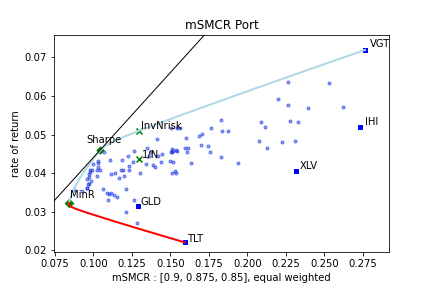
\includegraphics[width=.95\linewidth]{../figs/mSMCRFrontier1.png}
  \caption{Rate of return vs. \mSMCR}
  \label{SMCR_fig1a}
\end{subfigure}%
\begin{subfigure}{.5\textwidth}
  \centering
  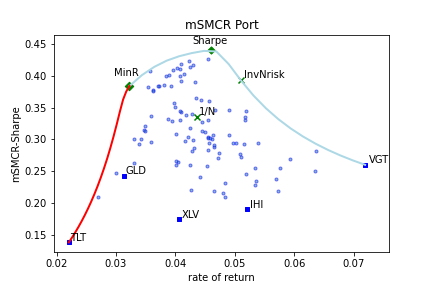
\includegraphics[width=.95\linewidth]{../figs/mSMCRFrontier2.png}
  \caption{\mSMCR-Sharpe vs. rate of return}
  \label{SMCR_fig1b}
\end{subfigure}
\caption{\mSMCR\ : [$\alpha=(0.9, 0.875, 0.85)$, equal weighted] frontiers.}
\label{SMCR_fig1}
\end{figure}

\BackToContents

\subsubsection{Backtesting mSMCR-Sharpe optimal portfolio}

Here is an example, using \azapy\ package, of computing a portfolio backtesting.
For this example, we have chosen a portfolio quarterly rebalanced according
to the maximization of \mSMCR-Sharpe ratio. At each rebalancing date,
the portfolio weights
are calibrated based on 3.25 years of prior historical market data (default settings).

Other rebalancing strategies can be considered
by changing the value of {\it rtype} parameter in the call of {\it set\_model} function below.
For more details see the package documentation at \azapydoc.

\lstinputlisting[language=Python]{../PyScripts/SMCR_Port.py}

\begin{figure}[H]
    \centering
    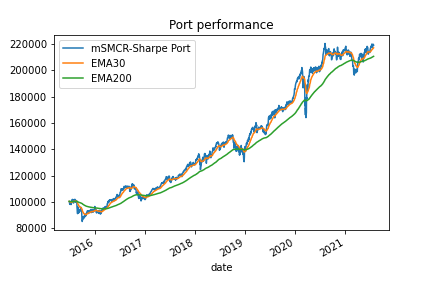
\includegraphics[width=.95\linewidth]{../figs/Port_mSMCR_Sharpe.png}
    \caption{Backtesting of quarterly rebalanced \mSMCR-Sharpe optimal portfolio,
    \mSMCR\ : [$\alpha=(0.975, 0.95, 0.9)$, equal weighted].}
    \label{SMCR_Port_fig}
\end{figure}

\BackToContents





\section{Downside dispersion measures}\label{mHMDD}

The m-level High Moment Downside Dispersion measure is defined as
\begin{equation}
    \mHMDD^{(p)}(r) = \sum_{l=1}^L \cK_l \times \delta^{(p)}_l(r),
    \label{hmdd1}
\end{equation}
where $\{\cK_l\}_{l=1,\cdots,L}$ is a positive non-increasing set of parameters normalized to unit
and $\delta^{(p)}_l$ is the $l$-th level delta-risk of rank $p$, recursively defined as
\begin{align}
    \delta^{(p)}_1(r) &= \left\| \left( -\br \right)^+ \right\|_p, \label{hmdd3} \\
    \cdots & \nonumber \\
    \delta^{(p)}_L(r)  &= \left\| \left( -\br - \sum_{j=1}^{L-1} \delta^{(p)}_j \right)^+ \right\|_p, \label{hmdd2}
\end{align}
where $\br = r - \mE[r]$ is the detrended rate of return and
$\|\cdot\|_p= \left(\mE[(|\cdot|^p)]\right)^{1/p}$ is the $L^p$-norm.
$\mHMDD^{(p)}$ are genuine dispersion measures.

The most famous member of this family of dispersion measures is the m-level Mean Absolute Deviation, \mMAD,
introduced in 2001 by Michalowski and Ogryczak \cite{Ogryczak}.
Another important member is m-level Lower Semi-Deviation, \mLSD.

Relative to the family of downside dispersion measures, \mMAD\ and \mLSD\ are the first, $p=1$, and
second, $p=2$, moment downside dispersion measures, respectively, \ie,
\begin{align}
    \mMAD(r) &\equiv \mHMDD^{(1)}(r), \label{hmdd4} \\
    \mLSD(r) &\equiv \mHMDD^{(2)}(r). \label{hmdd5}
\end{align}
Optimal portfolio strategies based on these two measures are presented separately in the next two subsections.

\BackToContents


\subsection{mMAD-based optimization strategies}\label{S:mMAD}

\MAD\ stands for Mean Absolute Deviation. It is a genuine dispersion measure.
It was introduced by Konno and Yamarzaki in 1991 \cite{Konno} as an alternative to more familiar
variance from mean-variance Markovitz model \cite{Markowitz}.
From a numerical point of view, \MAD-based portfolio optimizations can be expressed as LP while
\MV\ (variance) based portfolio optimizations as QP/SOCP problems. Therefore, the perception that an \MAD-based optimization strategy could
be more easily tractable than its \MV\ equivalent.
In its initial form, the \MAD\ dispersion measure was defined as
\begin{equation}
    \MAD(r) = \mE\left[ \left| r - \mE[r]  \right| \right].
\end{equation}
\MAD\ is not a downside dispersion measure per se. Same as variance, it is a central momentum dispersion measure (see Sec.~\ref{CentralM}), penalizing equally the under and over
realizations relative to the mean.

However, once was recognized that
\begin{equation}
    \mE\left[ \left| r - \mE[r] \right| \right] = 2 \mE\left[ \left( \mE[r] - r \right)^+ \right],
\end{equation}
\MAD\ was extended to m-level \MAD\ dispersion measure (for short \mMAD) in 2001 by Michalowski and Ogryczak \cite{Ogryczak}.
\mMAD\ can be defined as the first order \mHMDD, $p=1$ in Eq.~(\ref{hmdd1}), \ie,
\begin{equation}
    \mMAD(r) = \sum_{l=1}^L \cK_l \times \delta^{(1)}_l(r).
    \label{mmad0}
\end{equation}
where $\{\cK_l\}_{l=1,\cdots,L}$ is a positive non-increasing set of coefficients normalized to unit and
$\delta^{(1)}_l$ is the $l$-th level delta-risk of first rank, recursively defined as
\begin{align}
    \delta^{(1)}_1(r) &= \mE \left[ \left( -\br \right)^+ \right], \label{mmad02} \\
    \cdots & \nonumber \\
    \delta^{(1)}_L(r)  &= \mE \left[ \left( -\br - \sum_{j=1}^{L-1} \delta^{(1)}_j \right)^+ \right], \label{mmad01}
\end{align}
with $\br = r - \mE[r]$ the detrended rate of return.

For higher levels, $L>1$, \mMAD\ is a genuine downside dispersion measure, adding more weight to downside observations below the mean.
The weights associated to extreme events are increasing with the size of $L$.

\BackToContents

\subsubsection{mMAD dispersion measure}
The numerical computation of \mMAD, from Eq.~(\ref{mmad0}), is straightforward.
Let $L$ by the highest level involved in the expression of \mMAD. Then,
the set of $\{\delta^{(1)}_l\}_{l=1,\cdots,L}$ is evaluated recursively as
\begin{equation}
    \delta^{(1)}_l = \frac{1}{N}\sum_{i=1}^N \left( -\br_i -\sum_{j=1}^{l-1} \delta^{(1)}_j \right)^+.
    \label{mmad1}
\end{equation}
The $\mMAD$ is given by the sum from Eq.~(\ref{mmad0}).

\BackToContents

\subsubsection{mMAD optimal portfolio}
The optimization is described by Eqs.~(\ref{gg1}) from Sec.~\ref{strategies} point~\ref{OptRisk},
where $\rho$ is given by \mMAD\ from Eq.~(\ref{mmad0}).
It is the following LP problem.

\bigskip
\noindent Minimize over $\{ \{w_k\}_{k=1,\cdots,M}, \{ \eta_l, \{ s_{li} \}_{i=1,\cdots,N} \}_{l=1,\cdots,L} \}$
\begin{subequations}\label{mmad2}
\begin{align}
    &g = \sum_{l=1}^L \cK_l \eta_l, \label{mmad2a} \\
    \st &\frac{1}{N} \sum_{i=1}^N s_{li} = \eta_l, \label{mmad2b} \\
        &s_{li} + \sum_{k=1}^M w_k \br_{ki} + \sum_{j=1}^{l-1} \eta_j \geq 0, \label{mmad2c} \\
        &\sum_{k=1}^M w_k \mu_k \geq \mu, \label{mmad2d} \\
        &\sum_{k=1}^M w_k = 1, \label{mmad2e} \\
        & s_{li} \geq 0, \label{mmad2f} \\
        &\eta_l \geq 0, \label{mmad2h} \\
        & w_k \geq 0, \label{mmad2g}
\end{align}
\end{subequations}

\noindent where $\mu$ from Eq.~(\ref{mmad2d}) is the portfolio targeted expected rate of return, while $\{\mu_k\}_{k = 1,\cdots,M}$
are the portfolio components expected rate of returns.
Then, we have
\begin{subequations}\label{mmad3}
\begin{align}
    \RR &= \sum_{k=1}^M w_k^* \mu_k, \label{mmad3a} \\
    \mMAD &= g^*, \label{mmad3b} \\
    \delta^{(1)}_l &= \eta_l^*, \label{mmad3c}
\end{align}
\end{subequations}

\noindent where $^*$ denotes the solution of LP problem.
In addition to the optimal portfolio weights $\{w_k^*\}_{k=1,\cdots,M}$ and
expected rate of return $\RR$, the
LP solution provides information about the portfolio \mMAD\ and its delta-risk components.

\bigskip
\noindent Here is an example, using the \azapy\ package, of how to compute the \mMAD\ optimal portfolio.
The \mMAD\ time horizon was set to one quarter and the calibration is performed using the prior 3.25 years of
close-adjusted historical prices (default settings).
For more details see the package documentation at \azapydoc.

\lstinputlisting[language=Python]{../PyScripts/MAD_RiskOptim.py}

\BackToContents

\subsubsection{Minimum mMAD portfolio}

Following the result from Sec.~\ref{strategies} point~\ref{MinRisk},
the algorithm to compute the optimal portfolio with minimum \mMAD\ is given by Eqs.~(\ref{mmad2}) where
$\mu$ from r.h.s. of Eq.~(\ref{mmad2d}) is set to a value equal to the smallest expected rate of
return among the portfolio components, \ie\ $\mu=\min_k\{\mu_k\}$.

\bigskip
\noindent Here is an example, using the \azapy\ package, of how to compute the minimum \mMAD\ portfolio.
The \mMAD\ time horizon was set to one quarter and the calibration is performed using the prior 3.25 years of
close-adjusted historical prices (default settings).
For more details see the package documentation at \azapydoc.

\lstinputlisting[language=Python]{../PyScripts/MAD_MinRisk.py}

\BackToContents

\subsubsection{mMAD optimal portfolio for targeted risk value}
This optimization is described by Eqs.~(\ref{gg2}) from Sec.~\ref{strategies} point~\ref{TargetRisk},
where $\rho$ is given by $\mMAD$ from Eq.\ (\ref{mmad0}).
It is the following LP problem.

\bigskip
\noindent Maximize over $\{ \{w_k\}_{k=1,\cdots,M}, \{ \eta_l, \{ s_{li} \}_{i=1,\cdots,N} \}_{l=1,\cdots,L} \}$
\begin{subequations}\label{mmad4}
\begin{align}
    &g = \sum_{k=1}^M \mu_k w_k, \label{mmad4a} \\
    \st &\sum_{l=1}^L\cK_l \eta_l = \mMAD_0, \label{mmad4d} \\
        &\frac{1}{N} \sum_{i=1}^N s_{li} = \eta_l, \label{mmad4b} \\
        &s_{li} + \sum_{k=1}^M w_k \br_{ki} + \sum_{j=1}^{l-1} \eta_j \geq 0, \label{mmad4c} \\
        &\sum_{k=1}^M w_k = 1, \label{mmad4e} \\
        & s_{li} \geq 0, \label{mmad4f} \\
        &\eta_l \geq 0, \label{mmad4h} \\
        & w_k \geq 0, \label{mmad4g}
\end{align}
\end{subequations}

\noindent where $\mMAD_0$ in Eq.~(\ref{mmad4d}) is the portfolio targeted \mMAD\ dispersion value.
Then, we have
\begin{subequations}\label{mmad5}
\begin{align}
    \RR &= g^*, \label{mmad5a} \\
    \delta^{(1)}_l &= \eta_l^*, \label{mmad5b}
\end{align}
\end{subequations}

\noindent where $^*$ denotes the solution of LP problem.
In addition to the optimal portfolio weights $\{w_k^*\}_{k=1,\cdots,M}$ and expected rate of return $\RR$,
the solution of LP problem provides information about the $\mMAD_0$ delta-risk components values,
although, this information is likely to be known at the outset.

\bigskip
\noindent Here is an example, using the \azapy\ package, of how to compute the optimal portfolio
with the same $\mMAD$ as the equal weighted portfolio.
The \mMAD\ time horizon was set to one quarter and the calibration is performed using the prior 3.25 years of
close-adjusted historical prices (default settings).
For more details see the package documentation at \azapydoc.

\lstinputlisting[language=Python]{../PyScripts/MAD_InvNrisk.py}

\BackToContents

\subsubsection{mMAD optimal portfolio for fixed risk-aversion factor}
This optimization is described by Eqs.~(\ref{gg3}) from Sec.~\ref{strategies} point~\ref{RiskAverse},
where $\rho$ is given by \mMAD\ from Eq.~(\ref{mmad0}).
It is the following LP problem.

\bigskip
\noindent Maximize over $\{ \{w_k\}_{k=1,\cdots,M}, \{ \eta_l, \{ s_{li} \}_{i=1,\cdots,N} \}_{l=1,\cdots,L} \}$
\begin{subequations}\label{mmad6}
\begin{align}
    &g = \sum_{k=1}^M w_k\mu_k - \lambda \sum_{l=1}^L \cK_l \eta_l, \label{mmad6a} \\
    \st &\frac{1}{N} \sum_{i=1}^N s_{li} = \eta_l, \label{mmad6b} \\
        &s_{li} + \sum_{k=1}^M w_k \br_{ki} + \sum_{j=1}^{l-1} \eta_j \geq 0, \label{mmad6c} \\
        &\sum_{k=1}^M w_k = 1, \label{mmad6d} \\
        & s_{li} \geq 0, \label{mmad6e} \\
        &\eta_l \geq 0, \label{mmad6g} \\
        & w_k \geq 0, \label{mmad6f}
\end{align}
\end{subequations}

\noindent where $\lambda$ from Eqs.~(\ref{mmad6a}) is the risk-aversion factor.
Then, we have
\begin{subequations}\label{mmad7}
\begin{align}
    \RR &= \sum_{k=1}^M w_k^* \mu_k, \label{mmad7a} \\
    \mMAD &= \frac{\RR - g^*}{\lambda}, \label{mmad7b} \\
    \delta^{(1)}_l &= \eta_l^*, \label{mmad7c}
\end{align}
\end{subequations}

\noindent where $^*$ denotes the solution of LP problem.
In addition to the optimal portfolio weights $\{w_k^*\}_{k=1,\cdots,M}$ and expected rate of return $\RR$,
the LP solution provides information about \mMAD\ and its delta-risk components values.

\bigskip
\noindent Here is an example, using the \azapy\ package, of how to compute the optimal portfolio
for a given value of the risk-aversion factor $\lambda$.
The \mMAD\ time horizon was set to one quarter and the calibration is performed using the prior 3.25 years of
close-adjusted historical prices (default settings).
For more details see the package documentation at \azapydoc.

\lstinputlisting[language=Python]{../PyScripts/MAD_Averse.py}

\BackToContents

\subsubsection{mMAD-Sharpe optimal portfolio - maximization solution}
This optimization targets the maximization of \mMAD-Sharpe ratio. It is based on the
Eqs.~(\ref{gg4}) from Sec.~\ref{strategies} point~\ref{MaxSharpe}, where $\rho$ is given by \mMAD\ from Eq.~(\ref{mmad0}).
The optimization can be formulated as an LP problem if Eq.~(\ref{gg4b}) can be linearized.
In our case the linearization is straightforward. Introducing the following
variable transformations $\bw_k = t w_k$, $\bs_{li} = t s_{li}$ and $\bbeta_l = t \eta_l$, the LP
problem can be written as follows.

\bigskip
\noindent Maximize over $\{ \{\bw_k\}_{k=1,\cdots,M}, \{ \bbeta_l, \{ \bs_{li} \}_{i=1,\cdots,N} \}_{l=1,\cdots,L}, t \}$
\begin{subequations}\label{mmad8}
\begin{align}
    &g =\sum_{k=1}^M \mu_k \bw_k - \mu_0 t, \label{mmad8a} \\
    \st &\sum_{l=1}^L \cK_l \bbeta_l = 1, \label{mmad8d} \\
        &\frac{1}{N} \sum_{i=1}^N \bs_{li} = \bbeta_l, \label{mmad8b} \\
        &\bs_{li} + \sum_{k=1}^M \bw_k \br_{ki} + \sum_{j=1}^{l-1} \bbeta_j \geq 0, \label{mmad8c} \\
        &\sum_{k=1}^M \bw_k - t = 0, \label{mmad8e} \\
        &t \geq 0, \label{mmad8i} \\
        &\bs_{li} \geq 0, \label{mmad8f} \\
        &\bbeta_l \geq 0, \label{mmad8h} \\
        &\bw_k \geq 0, \label{mmad8g}
\end{align}
\end{subequations}

\noindent where $\mu_0$ from Eq.~(\ref{mmad8a}) is the risk-free rate accessible to the investor.
Then, we have
\begin{subequations}\label{mmad9}
\begin{align}
    w_k &= \frac{\bw_k^*}{t^*} , \label{mmad9a} \\
    \RR &= \frac{g^*}{t^*} + \mu_0, \label{mmad9b} \\
    \Sharpe &= g^*, \label{mmad9c} \\
    \mMAD &= \frac{1}{t^*}, \label{mmad9d} \\
    \delta^{(1)}_l &= \frac{\bbeta_l^*}{t^*}, \label{mmad9e}
\end{align}
\end{subequations}

\noindent where $^*$ denotes the solution of LP problem.
In addition to the optimal portfolio weights $\{w_k\}_{k=1,\cdots,M}$, expected rate of return $\RR$ and
\mMAD-Sharpe ratio $\Sharpe$,
the LP solution provides information about \mMAD\ and its delta-risk components.

\bigskip
\noindent Here is an example, using the \azapy\ package, of how to compute the \mMAD-Sharpe optimal portfolio using the maximization
of \mMAD-Sharpe ratio.
The \mMAD\ time horizon was set to one quarter and the calibration is performed using the prior 3.25 years of
close-adjusted historical prices (default settings).
For more details see the package documentation at \azapydoc.

\lstinputlisting[language=Python]{../PyScripts/MAD_Sharpe.py}

\BackToContents


\subsubsection{mMAD-Sharpe optimal portfolio - minimization solution}
This optimization targets the minimization of the inverse of \mMAD-Sharpe ratio.
It is described by Eqs.~(\ref{gg8}) from Sec.~\ref{strategies} point~\ref{MinSharpe}, where
$\rho$ is given by \mMAD\ from Eq.~(\ref{mmad0}).
The optimization can be formulated as an LP problem if Eq.~(\ref{gg8a}) can be linearized. This can be achieved by
introducing the variable transformations
$\bw_k = t w_k$, $\bs_{li} = t s_{li}$ and $\bbeta_l = t \eta_l$.
Then, the LP problem can be written as follows.

\bigskip
\noindent Minimize over $\{ \{\bw_k\}_{k=1,\cdots,M}, \{ \bbeta_l, \{ \bs_{li} \}_{i=1,\cdots,N} \}_{l=1,\cdots,L}, t \}$
\begin{subequations}\label{mmad10}
\begin{align}
    &g = \sum_{l=1}^L \cK_l \bbeta_l, \label{mmad10a} \\
    \st &\frac{1}{N} \sum_{i=1}^N \bs_{li} = \bbeta_l, \label{mmad10b} \\
        &\bs_{li} + \sum_{k=1}^M \bw_k \br_{ki} + \sum_{j=1}^{l-1} \bbeta_j \geq 0, \label{mmad10c} \\
        &\sum_{k=1}^M \mu_k \bw_k -\mu_0 t = 1, \label{mmad10d} \\
        &\sum_{k=1}^M \bw_k - t = 0, \label{mmad10e} \\
        & t \geq 0, \label{mmad10h} \\
        &\bs_{li} \geq 0, \label{mmad10f} \\
        &\bbeta_l \geq 0, \label{mmad10i} \\
        &\bw_k \geq 0, \label{mmad10g}
\end{align}
\end{subequations}

\noindent where $\mu_0$ from Eq.~(\ref{mmad10d}) is the risk-free rate accessible to the investor.
Then, we have
\begin{subequations}\label{mmad11}
\begin{align}
    w_k &= \frac{\bw_k^*}{t^*} , \label{mmad11a} \\
    \RR &= \frac{1}{t^*} + \mu_0, \label{mmad11b} \\
    \Sharpe &= \frac{1}{g^*}, \label{mmad11c} \\
    \mMAD &= \frac{g^*}{t^*}, \label{mmad11d} \\
    \delta^{(1)}_l &= \frac{\bbeta_l^*}{t^*} , \label{mmad11e}
\end{align}
\end{subequations}

\noindent where $^*$ denotes the solution of LP problem.
In addition to the optimal portfolio weights $\{w_k\}_{k=1,\cdots,M}$, expected rate of return $\RR$ and
\mMAD-Sharpe ratio $\Sharpe$,
the LP solution provides information about \mMAD\ and its delta-risk components.


\bigskip
\noindent Here is an example, using the \azapy\ package, of how to compute the \mMAD-Sharpe optimal portfolio using the minimization
of the inverse of \mMAD-Sharpe ratio.
The \mMAD\ time horizon was set to one quarter and the calibration is performed using the prior 3.25 years of
close-adjusted historical prices (default settings).
For more details see the package documentation at \azapydoc.

\lstinputlisting[language=Python]{../PyScripts/MAD_InvSharpe.py}

\BackToContents

\subsubsection{mMAD frontiers}

Here is an example of how to compute the \mMAD\ frontiers using the \azapy\
package. The \mMAD\ time horizon was set to one quarter and the calibration is performed using the prior 3.25 years of
close-adjusted historical prices (default settings).
For more details see the package documentation at \azapydoc.

The script will produce the plots in Figs. \ref{MAD_fig1a} and \ref{MAD_fig1b}
for historical data collected up to 2021-07-27.


\lstinputlisting[language=Python]{../PyScripts/MAD_frontiers.py}

\begin{figure}[H]
\centering
\begin{subfigure}{.5\textwidth}
  \centering
  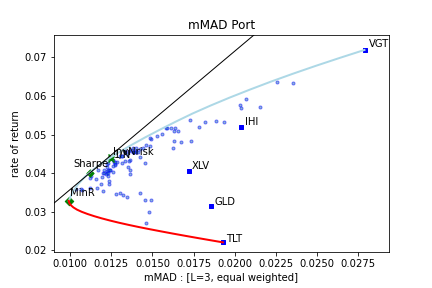
\includegraphics[width=.95\linewidth]{../figs/mMADFrontier1.png}
  \caption{Rate of return vs. \mMAD}
  \label{MAD_fig1a}
\end{subfigure}%
\begin{subfigure}{.5\textwidth}
  \centering
  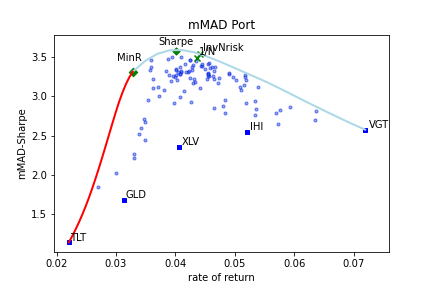
\includegraphics[width=.95\linewidth]{../figs/mMADFrontier2.png}
  \caption{\mMAD-Sharpe vs. rate of return}
  \label{MAD_fig1b}
\end{subfigure}
\caption{\mMAD : [L=3, equal weighted]  frontiers.}
\label{MAD_fig1}
\end{figure}

\BackToContents

\subsubsection{Backtesting mMAD-Sharpe optimal portfolio}

Here is an example, using \azapy\ package, of computing a portfolio backtesting.
For this example, we have chosen a portfolio quarterly rebalanced according
to the maximization of \mMAD-Sharpe ratio. At each rebalancing date,
the portfolio weights
are calibrated based on 3.25 years of prior historical market data.

Other rebalancing strategies can be considered
by changing the value of {\it rtype} parameter in the call of {\it set\_model} function below.
For more details see the package documentation at \azapydoc.

\lstinputlisting[language=Python]{../PyScripts/MAD_Port.py}

\begin{figure}[H]
    \centering
    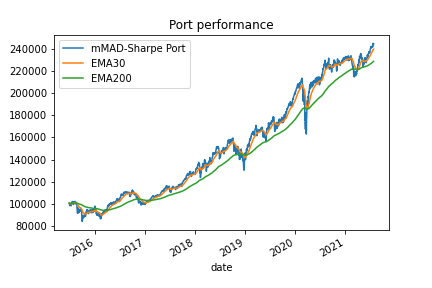
\includegraphics[width=.95\linewidth]{../figs/Port_mMAD_Sharpe.png}
    \caption{Backtesting of quarterly rebalanced \mMAD-Sharpe optimal portfolio,
    \mMAD\ : [L=3, equal weighted].}
    \label{MAD_Port_fig}
\end{figure}

\BackToContents





\subsection{mLSD-based optimization strategies}\label{S:mLSD}

\LSD\ stands for Lower Semi-Deviation. The \LSD\ dispersion measure can be defined as
\begin{equation}
    \LSD(r) = \left\| \left(-\br \right)^+ \right\|_2,
    \label{LSD:1}
\end{equation}
where $\br = r - \mE[r]$ is the detrended rate of return and $\|\cdot\|_2 = (\mE[|\cdot|^2])^{1/2}$ is the $L^2$-norm.

Unlike \MAD, \LSD\ is a genuine downside dispersion measure.
The \LSD-based portfolio optimization strategies were studied mainly through its
cousin, the semi-variance dispersion measure, the square of \LSD, introduced in 1959 by Markowitz \cite{Markowitz2}.
Note that semi-variance is not a genuine dispersion measure. It violates the
positive homogeneity axiom.
Nevertheless, the \LSD\ and the semi-variance optimal portfolios are the same.\footnote{Similar remarks with those made in
Sec.~\ref{CentralM} about variance and standard deviation based portfolio optimization strategies hold here.}

Like \MAD, \LSD\ can be extended to m-level \LSD. The \mLSD\ dispersion measure
is the m-level second moment downside dispersion measure from Eq.~(\ref{hmdd5}), \ie,
\begin{equation}
    \mLSD(r) = \sum_{l=1}^L \cK_l \times \delta^{(2)}_l(r),
    \label{LSD0}
\end{equation}
where $\{\cK_l\}_{l=1,\cdots,L}$ is a positive non-increasing set of coefficients normalized to unit and
$\delta^{(2)}_l$ is the $l$-th level delta-risk of second rank,
recursively defined as
\begin{align}
    \delta^{(2)}_1(r) &= \left\| \left(-\br \right)^+ \right\|_2, \label{LSD02} \\
    \cdots & \noindent \\
    \delta^{(2)}_L(r) &= \left\| \left(-\br - \sum_{j=1}^{L-1} \delta^{(2)}_j \right)^+ \right\|_2. \label{LSD01}
\end{align}


\BackToContents


\subsubsection{mLSD dispersion measure}
The numerical computation of \mLSD\ from Eq.~(\ref{LSD0}) is straightforward.
Let $L$ by the highest level involved in the expression of \mLSD. Then,
the set of $\{\delta^{(2)}_l\}_{l=1,\cdots,L}$ are evaluated recursively as follows
\begin{equation}
    \delta^{(2)}_l = \left(\frac{1}{N}\sum_{i=1}^N \left[\left( -\br_i -\sum_{j=1}^{l-1} \delta^{(2)}_j \right)^+\right]^2 \right)^{1/2}.
    \label{LSD1}
\end{equation}
The \mLSD\ is given by the sum from Eq.~(\ref{LSD0}).

\BackToContents

\subsubsection{mLSD optimal portfolio}
This optimization is described by Eqs.\ (\ref{gg1}) from Sec.~\ref{strategies} point~\ref{OptRisk},
where $\rho$ is given by \mLSD\ from Eq.~(\ref{LSD0}).
It is the following SOCP problem.

\bigskip
\noindent Minimize over $\{ \{w_k\}_{k=1,\cdots,M}, \{ \eta_l, \{ s_{li} \}_{i=1,\cdots,N} \}_{l=1,\cdots,L} \}$
\begin{subequations}\label{LSD2}
\begin{align}
    & g = \sum_{l=1}^L \cK_l \eta_l, \label{LSD2a} \\
    \st & \left( \frac{1}{N} \sum_{i=1}^N s_{li}^2 \right)^{1/2} \leq \eta_l, \label{LSD2b} \\
        & s_{li} + \sum_{k=1}^M w_k\br_{ki} + \sum_{j=1}^{l-1}\eta_j \geq 0, \label{LSD2c} \\
        & \sum_{k=1}^M w_k \mu_k \geq \mu, \label{LSD2d} \\
        & \sum_{k=1}^M w_k = 1, \label{LSD2e} \\
        & s_{li} \geq 0, \label{LSD2f} \\
        & \eta_l \geq 0, \label{LSD2h} \\
        & w_k \geq 0, \label{LSD2g}
\end{align}
\end{subequations}

\noindent where $\mu$ in Eq.~(\ref{LSD2d}) is the targeted portfolio expected rate of return while $\{\mu_k\}_{i=1,\cdots,M}$
are the portfolio components expected rate of returns.
Then, we have
\begin{subequations}\label{LSD3}
\begin{align}
    \RR &= \sum_{k=1}^m w_k^* \mu_k, \label{LSD3a} \\
    \mLSD &= g^*, \label{LSD3b} \\
    \delta^{(2)}_l & = \eta_l^*, \label{LSD3c}
\end{align}
\end{subequations}

\noindent where $^*$ denotes the solution of SOCP problem.
In addition to the portfolio weights $\{w_k^*\}_{k=1,\cdots,M}$ and optimal portfolio expected rate of return $\RR$,
the SOCP solution provides information about the portfolio \mLSD\ and its delta-risk
components.


\bigskip
\noindent Here is an example, using the \azapy\ package, of how to compute the \mLSD\ optimal portfolio.
The \mLSD\ time horizon was set to one quarter and the calibration is performed using the prior 3.25 years of
close-adjusted historical prices (default settings).
For more details see the package documentation at \azapydoc.

\lstinputlisting[language=Python]{../PyScripts/LSD_RiskOptim.py}

\BackToContents

\subsubsection{Minimum mLSD portfolio}
Following the results from Sec.~\ref{strategies} point~\ref{MinRisk}, the
algorithm to compute the optimal portfolio with minimum \mLSD\ is given by Eqs.~(\ref{LSD2}) where
$\mu$ from r.h.s. of Eq.~(\ref{LSD2d}) is set to a value equal to the smallest expected rate of
return among the portfolio components, \ie\ $\mu=\min_k\{\mu_k\}$.

\bigskip
\noindent Here is an example, using the \azapy\ package, of how to compute the minimum \mLSD\ portfolio.
The \mLSD\ time horizon was set to one quarter and the calibration is performed using the prior 3.25 years of
close-adjusted historical prices (default settings).
For more details see the package documentation at \azapydoc.

\lstinputlisting[language=Python]{../PyScripts/LSD_MinRisk.py}

\BackToContents

\subsubsection{mLSD optimal portfolio for targeted risk value}
This optimization is given by Eqs.~(\ref{gg2}) from Sec.~\ref{strategies} point~\ref{TargetRisk}, where $\rho$ is
given by $\mLSD$ from Eq.~(\ref{LSD0}).
It is the following SOCP problem.

\bigskip
\noindent Maximize over $\{ \{w_k\}_{k=1,\cdots,M}, \{ \eta_l, \{ s_{li} \}_{i=1,\cdots,N} \}_{l=1,\cdots,L} \}$
\begin{subequations}\label{LSD4}
\begin{align}
    & g = \sum_{k=1}^M w_k \mu_k, \label{LSD4a} \\
    \st & \left( \frac{1}{N} \sum_{i=1}^N s_{li}^2 \right)^{1/2} \leq \eta_l, \label{LSD4b} \\
        & s_{li} + \sum_{k=1}^M w_k\br_{ki} + \sum_{j=1}^{l-1}\eta_j \geq 0, \label{LSD4c} \\
        & \sum_{l=1}^L \cK_l \eta_l = \mLSD_0, \label{LSD4d} \\
        & \sum_{k=1}^M w_k = 1, \label{LSS4e} \\
        & s_{li} \geq 0, \label{LSD4f} \\
        & \eta_l \geq 0, \label{LSD4h} \\
        & w_k \geq 0, \label{LSD4g}
\end{align}
\end{subequations}

\noindent where $\mLSD_0$ in Eq.~(\ref{LSD4d}) is the portfolio targeted \mLSD\ dispersion value.
Then, we have
\begin{subequations}\label{LSD5}
\begin{align}
    \RR &= g^*, \label{LSD5a} \\
    \delta^{(2)}_l & = \eta_l^*, \label{LSD5b}
\end{align}
\end{subequations}

\noindent where $^*$ denotes the solution of SCOP problem.
In addition to the optimal portfolio weights $\{w_k^*\}_{k=1,\cdots,M}$ and expected rate of return $\RR$,
the SOCP solution provides information about the $\delta^{(2)}_l$ components of $\mLSD_0$,
although, this information is likely to be known at the outset.

\bigskip
\noindent Here is an example, using the \azapy\ package, of how to compute the optimal portfolio
with the same \mLSD\ as the equal weighted portfolio.
The \mLSD\ time horizon was set to one quarter and the calibration is performed using the prior 3.25 years of
close-adjusted historical prices (default settings).
For more details see the package documentation at \azapydoc.

\lstinputlisting[language=Python]{../PyScripts/LSD_InvNrisk.py}

\BackToContents

\subsubsection{mLSD optimal portfolio for fixed risk-aversion factor}
This optimization is described by Eqs.~(\ref{gg3}) from Sec.~\ref{strategies} point~\ref{RiskAverse},
where $\rho$ is given by \mLSD\ from Eq.~(\ref{LSD0}).
It is the following SOCP problem.

\bigskip
\noindent Maximize over $\{ \{w_k\}_{k=1,\cdots,M}, \{ \eta_l, \{ s_{li} \}_{i=1,\cdots,N} \}_{l=1,\cdots,L} \}$
\begin{subequations}\label{LSD6}
\begin{align}
    & g = \sum_{k=1}^M w_k\mu_k - \lambda \sum_{l=1}^L \cK_l \eta_l, \label{LSD6a} \\
    \st & \left( \frac{1}{N} \sum_{i=1}^N s_{li}^2 \right)^{1/2} \leq \eta_l, \label{LSD6b} \\
        & s_{li} + \sum_{k=1}^M w_k\br_{ki} + \sum_{j=1}^{l-1}\eta_j \geq 0, \label{LSD6c} \\
        &\sum_{k=1}^M w_k = 1, \label{LSD6d} \\
        & s_{li} \geq 0, \label{LSD6e} \\
        & \eta_l \geq 0, \label{LSD6g} \\
        & w_k \geq 0, \label{LSD6f}
\end{align}
\end{subequations}

\noindent where $\lambda$ from Eqs.~(\ref{LSD6a}) is the risk-aversion factor.
Then, we have
\begin{subequations}\label{LSD7}
\begin{align}
    \RR &= \sum_{k=1}^M w_k^* \mu_k, \label{LSD7a} \\
    \mLSD &= \frac{\RR - g^*}{\lambda}, \label{LSD7b} \\
    \delta^{(2)}_l &= \eta_l^*, \label{LSD7c}
\end{align}
\end{subequations}

\noindent where $^*$ denotes the solution of the SOCP problem.
In addition to the optimal portfolio weights $\{w_k^*\}_{k=1,\cdots,M}$ and expected rate of return $\RR$,
the SOCP solution provides information about the portfolio \mLSD\ and its delta-risk components.

\bigskip
\noindent Here is an example, using the \azapy\ package, of how to compute the optimal portfolio
for a given value of the risk-aversion factor.
The \mLSD\ time horizon was set to one quarter and the calibration is performed using the prior 3.25 years of
close-adjusted historical prices (default settings).
For more details see the package documentation at \azapydoc.

\lstinputlisting[language=Python]{../PyScripts/LSD_Averse.py}

\BackToContents

\subsubsection{mLSD-Sharpe optimal portfolio - maximization solution}
This optimization targets the maximization of \mLSD-Sharpe ratio. It is based on the
Eqs.~(\ref{gg4}) from Sec.~\ref{strategies} point~\ref{MaxSharpe},
where $\rho$ is given by \mLSD\ from Eq.~(\ref{LSD0}).
The optimization can be formulated as an SOCP problem if Eq.~(\ref{gg4b}) can be expressed as a second order cone constraint.
This can be achieved by
introducing the variable transformations $\bw_k = t w_k$, $\bs_{li} = t s_{li}$ and $\bbeta_l = t \eta_l$.
Then, the SOCP problem can be written as follows.

\bigskip
\noindent Maximize over $\{ \{\bw_k\}_{k=1,\cdots,M}, \{ \bbeta_l, \{ \bs_{li} \}_{i=1,\cdots,N} \}_{l=1,\cdots,L}, t \}$
\begin{subequations}\label{LSD8}
\begin{align}
    &  g = \sum_{k=1}^M \bw_k \mu_k - \mu_0 t, \label{LSD8a} \\
    \st & \left( \frac{1}{N} \sum_{i=1}^N \bs_{li}^2 \right)^{1/2} \leq \bbeta_l, \label{LSD8b} \\
        & \bs_{li} + \sum_{k=1}^M \bw_k\br_{ki} + \sum_{j=1}^{l-1}\bbeta_j \geq 0, \label{LSD8c} \\
        & \sum_{l=1}^L \cK_l \bbeta_l = 1, \label{LSD8d} \\
        & \sum_{k=1}^M \bw_k - t = 0, \label{LSD8e} \\
        & t \geq 0, \label{LSD8h} \\
        & \bs_{li} \geq 0, \label{LSD8f} \\
        & \bbeta_l \geq 0, \label{LSD8i} \\
        & \bw_k \geq 0, \label{LSD8g}
\end{align}
\end{subequations}

\noindent where $\mu_0$ from Eq.~(\ref{LSD8a}) is the risk-free rate accessible to the investor.
Then, we have
\begin{subequations}\label{LSD9}
\begin{align}
    w_k &= \frac{\bw_k^*}{t^*}, \label{LLSD9a} \\
    \RR &= \frac{g^*}{t^*} + \mu_0, \label{LSD9b} \\
    \Sharpe &= g^*, \label{LSD9c} \\
    \mLSD & = \frac{1}{t^*}, \label{LSD9d} \\
    \delta^{(2)}_l &= \frac{\bbeta_l^*}{t^*}, \label{LLSD9e}
\end{align}
\end{subequations}

\noindent where $^*$ denotes the solution of SOCP problem.
In addition to the optimal portfolio weights $\{w_k\}_{k=1,\cdots,M}$, expected rate of return $\RR$ and
\mLSD-Sharpe ratio $\Sharpe$,
the SOCP solution provides information about the portfolio \mLSD\ and its delta-risk components.

\bigskip
\noindent Here is an example, using the \azapy\ package, of how to compute the \mLSD-Sharpe optimal portfolio using the maximization
of \mLSD-Sharpe ratio.
The \mLSD\ time horizon was set to one quarter and the calibration is performed using the prior 3.25 years of
close-adjusted historical prices (default settings).
For more details see the package documentation at \azapydoc.

\lstinputlisting[language=Python]{../PyScripts/LSD_Sharpe.py}

\BackToContents


\subsubsection{mLSD-Sharpe optimal portfolio - minimization solution}
This optimization targets the minimization of the inverse of \mLSD-Sharpe ratio.
It is  described by Eqs.~(\ref{gg8}) from Sec.~\ref{strategies} point~\ref{MinSharpe}, where
$\rho$ is given by \mLSD\ from Eq.~(\ref{LSD0}).
The optimization can be formulated as an SOCP problem if  Eq.~(\ref{gg8a}) can be expressed as a second order cone constraint.
This can be achieved by
introducing the variable transformations
$\bw_k = t w_k$, $\bs_{li} = t s_{li}$ and $\bbeta_l = t \eta_l$.
Then, the SOCP problem can be written as follows.

\bigskip
\noindent Minimize over $\{ \{\bw_k\}_{k=1,\cdots,M}, \{ \bbeta_l, \{ \bs_{li} \}_{i=1,\cdots,N} \}_{l=1,\cdots,L}, t \}$
\begin{subequations}\label{LSD10}
\begin{align}
    & g = \sum_{l=1}^L \cK_l \bbeta_l, \label{LSD10a} \\
    \st & \left( \frac{1}{N} \sum_{i=1}^N \bs_{li}^2 \right)^{1/2} \leq \bbeta_l, \label{LSD10b} \\
        & \bs_{li} + \sum_{k=1}^M \bw_k\br_{ki} + \sum_{j=1}^{l-1}\bbeta_j \geq 0, \label{LSD10c} \\
        & \sum_{k=1}^M \bw_k \mu_k -\mu_0 t = 1, \label{LSD10d} \\
        & \sum_{k=1}^M \bw_k - t = 0, \label{LSD10e} \\
        & t \geq 0, \label{LSD10f} \\
        & \bs_{li} \geq 0, \label{LSD10g} \\
        & \bbeta_l \geq 0, \label{LSD11h} \\
        & \bw_k \geq 0, \label{LSD10i}
\end{align}
\end{subequations}

\noindent where $\mu_0$ from Eq.~(\ref{LSD10d}) is the risk-free rate accessible to the investor.
Then, we have
\begin{subequations}\label{LSD11}
\begin{align}
    w_k &= \frac{\bw_k^*}{t^*} , \label{LSD11a} \\
    \RR &= \frac{1}{t^*} + \mu_0, \label{LSD11b} \\
    \Sharpe &= \frac{1}{t^*}, \label{LSD11c} \\
    \mLSD &= \frac{g^*}{t^*}, \label{LSD11d} \\
    \delta^{(2)}_l &= \frac{\bbeta_l^*}{t^*}, \label{LSD11e}
\end{align}
\end{subequations}

\noindent where $^*$ denotes the solution of SOCP problem.
In addition to the optimal portfolio weights $\{w_k\}_{k=1,\cdots,M}$, expected rate of return $\RR$ and
\mLSD-Sharpe ratio $\Sharpe$,
the SOCP solution provides information about the portfolio \mLSD\ and its delta-risk components.

\bigskip
\noindent Here is an example, using the \azapy\ package, of how to compute the \mLSD-Sharpe optimal portfolio using the minimization
of the inverse of \mLSD-Sharpe ratio.
The \mLSD\ time horizon was set to one quarter and the calibration is performed using the prior 3.25 years of
close-adjusted historical prices (default settings).
For more details see the package documentation at \azapydoc.

\lstinputlisting[language=Python]{../PyScripts/LSD_InvSharpe.py}

\BackToContents

\subsubsection{mLSD frontiers}

Here is an example of how to compute the \mLSD\ frontiers using the \azapy\
package. The \mLSD\ time horizon was set to one quarter and the calibration is performed using the prior 3.25 years of
close-adjusted historical prices (default settings).
For more details see the package documentation at \azapydoc.

The script will produce the plots in Figs. \ref{LSD_fig1a} and \ref{LSD_fig1b}
for historical data collected up to 2021-07-27.

\lstinputlisting[language=Python]{../PyScripts/LSD_frontiers.py}

\begin{figure}[H]
\centering
\begin{subfigure}{.5\textwidth}
  \centering
  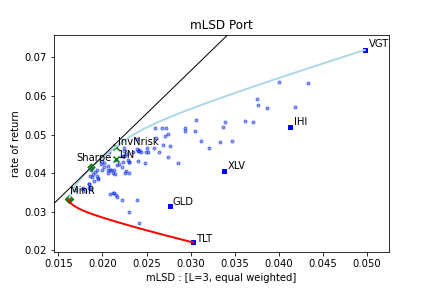
\includegraphics[width=.95\linewidth]{../figs/mLSDFrontier1.png}
  \caption{Rate of return vs. \mLSD}
  \label{LSD_fig1a}
\end{subfigure}%
\begin{subfigure}{.5\textwidth}
  \centering
  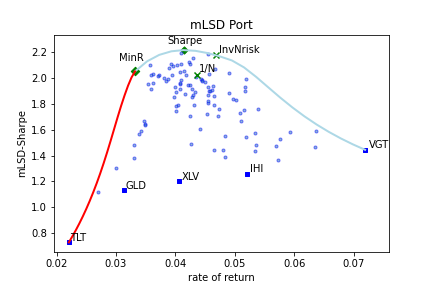
\includegraphics[width=.95\linewidth]{../figs/mLSDFrontier2.png}
  \caption{\mLSD-Sharpe vs. rate of return}
  \label{LSD_fig1b}
\end{subfigure}
\caption{\mLSD : [$L=3$, equal weighted], frontiers.}
\label{LSD_fig1}
\end{figure}

\BackToContents


\subsubsection{Backtesting mLSD-Sharpe optimal portfolio}

Here is an example, using \azapy\ package, of computing a portfolio backtesting.
For this example, we have chosen a portfolio quarterly rebalanced according
to the maximization of \mLSD-Sharpe ratio. At each rebalancing date,
the portfolio weights
are calibrated based on 3.25 years of prior historical market data.

Other rebalancing strategies can be considered
by changing the value of {\it rtype} parameter in the call of {\it set\_model} function below.
For more details see the package documentation at \azapydoc.

\lstinputlisting[language=Python]{../PyScripts/LSD_Port.py}

\begin{figure}[H]
    \centering
    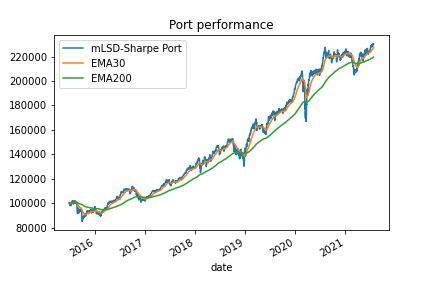
\includegraphics[width=.95\linewidth]{../figs/Port_mLSD_Sharpe.png}
    \caption{Backtesting of quarterly rebalanced \mLSD-Sharpe optimal portfolio,
    \mLSD\ : [$L=3$, equal weighted].}
    \label{LSD_Port_fig}
\end{figure}

\BackToContents



\section{Below threshold measures}
Below threshold measures, \BTM, can be defined as
\begin{equation}
    \BTM^{(p)}_\alpha = \left\| \left(\alpha - r\right)^+ \right\|_p,
    \label{btm1}
\end{equation}
where $\alpha \in \mR$ is the threshold and $\|\cdot\|_p = (\mE[|\cdot|^p])^{1/p}$ is the $L^p$-norm.

The most popular members of \BTM\ family are the \BTAD, Below Threshold Absolute Deviation, for $p=1$, and
\BTSD, Below Threshold Semi-Deviation, for $p=2$. However, famous are their corresponding generalized Sharpe ratios.
For $\mu_0=\alpha$,
\begin{itemize}
  \item \BTAD-Sharpe ratio is the Omega ratio,
  \item \BTSD-Sharpe ratio  is the Sortino ratio.
\end{itemize}
Both, Omega and Sortino optimal portfolio strategies are popular among practitioners.

In general, \BTM\ can be defined in terms of both standard rates of return $r$, as in Eq.~(\ref{btm1}), and
detrended rates of return, by replacing $r$ with $\br = r - \mE[r]$.
Expressed in terms of detrended rate of return and for $\alpha=0$, $\BTAD_0$ is equivalent to the first level \mMAD, $\delta^{(1)}_1$ from Eq.~(\ref{mmad0}),
while $\BTSD_0$ to the first level \mLSD, $\delta^{(2)}_1$ from Eq.~(\ref{LSD0}). In general, $\BTM^{(p)}_0$ (\ie\ for $\alpha=0$) with detrended rate of returns,
is equivalent to the first level $\mHMDD^{(p)}$, $\delta^{(p)}_1$ from Eq.~(\ref{hmdd1}).

Just as in the case of Tail dispersion measures, Eq.~(\ref{qq3}), \BTM\ can be extended to a mixture of $\BTM^{(p)}$ for different thresholds, \ie,
\begin{equation}
    \mBTM^{(p)} = \sum_{l=1}^L \cK_l \times \BTM^{(p)}_{\alpha_l},
    \label{btm2}
\end{equation}
where $\{\cK_l\}_{l=1,\cdots,L}$ is a set of positive mixture coefficients normalized to unit and
$\{\alpha_l\}_{l=1,\cdots,L}$ is a set of distinct thresholds.

Unlike the Tail and Downside measures, $\mBTM^{(p)}$ are not genuine dispersion measures.
They violate the positive homogeneity axiom and, in the case where standard rates of return are used, they also violate the location invariance.
An exception is the case where $L=1$ and $\alpha_1=0$ with detrended rate of return.
In this case $\mBTM^{(p)}$ becomes $\BTM^{(p)}_0$, which is a genuine dispersion measure.

However, the methodologies of optimal portfolio construction outlined in Sec.~\ref{strategies} can formally be applied to \mBTM.
They will be presented for \mBTAD\ (mixture \BTAD) and \mBTSD\ (mixture \BTSD) in the next two sections, respectively.

\BackToContents


\subsection{mBTAD-based optimization strategies}\label{S:mBTAD}

\BTAD\ stands for Below Threshold Absolute Deviation measure and is defined as
\begin{equation}
    \BTAD_\alpha = \mE\left[\left(\alpha - r\right)^+ \right],
    \label{oo1}
\end{equation}
where $\alpha \in \mR$ is called threshold.
The measure has gained in popularity after the introduction of
Omega ratio in 2002 by Keating and Shadwick \cite{Keating}.

Omega ratio is an investment performance measure. It was introduced as an alternative to Sharpe ratio
to measure expected excess return per unit of downside risk of realizations below a predefined threshold.
Over the years it has become very popular among practitioners.
It can be defined as\footnote{In the original paper of Keating and Shadwick \cite{Keating}, Omega ratio is defined without the $-1$.
It is a matter of convenience, adding or subtracting a constant from the ratio will not affect the optimal portfolio
composition. In our case it facilitates a readable expression for Eq.~(\ref{oo3}).}
\begin{equation}
    \Omega_{\mu_0} = \frac{\int_{\mu_0}^{+\infty} [1 - F(r)] dr}{\int_{-\infty}^{\mu_0} F(r) dr} - 1,
    \label{oo2}
\end{equation}
where $\mu_0$ is a constant called Omega threshold and $F(\cdot)$ is the portfolio rate of return cdf.
It is straightforward to show that $\Omega_{\mu_0}$ ratio can be expressed as
\begin{equation}
    \Omega_{\mu_0} = \frac{\mE(r) - \mu_0}{\mE[(\mu_0 - r)^+]}.
    \label{oo3}
\end{equation}
It is clear that the denominator from Eq.~(\ref{oo3}) is $\BTAD_{\mu_0}$. Therefore, Omega ratio can be viewed as
\BTAD-Sharpe ratio for $\alpha=\mu_0$.

As we mentioned in the preamble of this section, \BTAD\ can be defined in terms of both standard rate of return $r$ and
detrended rate of return $\br = r - \mE[r]$. In this subsection we will use the latter specification to write down the mathematical expressions. However, we should keep in
mind that, switching between the \BTAD\ definitions, is a simple matter of replacing $\br$ with $r$.\footnote{\azapy\ package provides a logical
flag to switch between the use of $r$ and $\br$ (see \azapydoc).}

Following the result from  Eq.~(\ref{btm2}), \mBTAD\ is defined as a superposition of \BTAD, \ie,
\begin{equation}
    \mBTAD = \sum_{l=1}^L \cK_l \times \BTAD_{\alpha_l},
    \label{oo0}
\end{equation}
where $\{\cK_l\}_{l=1,\cdots,L}$ is a set of positive constants normalized to unit (the mixture coefficients) and
$\{\alpha_l\}_{l=1,\cdots,L}$ is a set of distinct thresholds.

We will refer to the \mBTAD-Sharpe ratio as Omega ratio, since Omega ratio terminology is used more often among practitioners. However,
we should keep in mind, that our Omega ratio definition is equivalent to the original Keating and Shadwick \cite{Keating}
definition only in the case where $L=1$ and $\alpha_1 = \mu_0$ with standard rate of return.

In general, \mBTAD\ is not a genuine dispersion measure. It violates the positive homogeneity axiom and, in the case where standard rates of return
are used, it also violates local invariance. An exception is the case where $L=1$ and $\alpha_1=0$ with detrended rates of return.
In this case $\BTAD_0$ is equivalent to the first order \mMAD, delta-risk $\delta^{(1)}_1$ from Eq.~(\ref{mmad01}), which is a
genuine dispersion measure.

\BackToContents

\subsubsection{mBTAD dispersion measure}
The computation of the \BTAD\ is straightforward. Given a set $\{r_i\}_{i=1,\cdots,N}$ of observed rates or returns, we have
\begin{equation}
    \BTAD_\alpha = \frac{1}{N}\sum_{i=1}^N (\alpha - \br_i)^+.
    \label{btad01}
\end{equation}
Then, \mBTAD\ is given by the sum from Eq.~(\ref{oo0}).

\BackToContents

\subsubsection{mBTAD optimal portfolio}
The optimization is described by Eqs.~(\ref{gg1}) from Sec.~\ref{strategies} point~\ref{OptRisk},
where $\rho$ is given by \mBTAD\ from Eq.~(\ref{oo0}).
It is the following LP problem.

\bigskip
\noindent Minimize over $\{\{w_k\}_{k=1,\cdots,M}, \{ \eta_l, \{ s_{li} \}_{i=1,\cdots,N} \}_{l=1,\cdots,L} \}$,
\begin{subequations}\label{btad1}
\begin{align}
    &g = \sum_{l=1}^L \cK_l \eta_l, \label{btad1a} \\
    \st & \frac{1}{N} \sum_{i=1}^N s_{li} = \eta_l, \label{btad1b} \\
    & s_{li} + \sum_{k=1}^M w_k \br_{ki} \geq \alpha_l, \label{btad1c} \\
    & \sum_{k=1}^M w_k \mu_k \geq \mu, \label{btad1d} \\
    & \sum_{k=1}^M w_k = 1, \label{btad1e} \\
    & s_{li} \geq 0, \label{btad1g} \\
    & \eta_l \geq 0, \label{btad1h} \\
    & w_k \geq 0, \label{btad1f}
\end{align}
\end{subequations}

\noindent where $\mu$, in Eq.~(\ref{btad1d}), is the portfolio targeted expected rate of return, while $\mu_k$ for $k = 1,\cdots,M$
are the portfolio components expected rate of returns.
Then, we have
\begin{subequations}\label{btad2}
\begin{align}
    \RR &= \sum_{k=1}^M w_k^* \mu_k, \label{btad2a} \\
    \mBTAD &= g^*, \label{btad2b} \\
    \BTAD_{\alpha_l} &= \eta_l^*, \label{btad2c}
\end{align}
\end{subequations}

\noindent where $^*$ denotes the solution of LP problem.
In addition to the optimal portfolio weights $\{w_k^*\}_{k=1,\cdots,M}$ and
expected rate of return $\RR$, the
LP solution provides information about the portfolio \mBTAD\ and its components.

\bigskip
\noindent Here is an example, using the \azapy\ package, of how to compute the \mBTAD\ optimal portfolio.
The \mBTAD\ time horizon was set to one quarter and the calibration is performed using the prior 3.25 years of
close-adjusted historical prices (default settings).
For more details see the package documentation at \azapydoc.

\lstinputlisting[language=Python]{../PyScripts/BTAD_RiskOptim.py}

\BackToContents


\subsubsection{Minimum mBTAD portfolio}

Following the result from Sec.~\ref{strategies} point~\ref{MinRisk},
the algorithm to compute the optimal portfolio with minimum \mBTAD\ is given by Eqs.~(\ref{btad1}) where
$\mu$ from r.h.s. of Eq.~(\ref{btad1d}) is set to a value equal to the smallest expected rate of
return among the portfolio components, \ie\ $\mu=\min_k\{\mu_k\}$.

\bigskip
\noindent Here is an example, using the \azapy\ package, of how to compute the minimum \mBTAD\ portfolio.
The \mBTAD\ time horizon was set to one quarter and the calibration is performed using the prior 3.25 years of
close-adjusted historical prices (default settings).
For more details see the package documentation at \azapydoc.

\lstinputlisting[language=Python]{../PyScripts/BTAD_MinRisk.py}

\BackToContents

\subsubsection{mBTAD optimal portfolio for targeted risk value}
This optimization is described by Eqs.~(\ref{gg2}) from Sec.~\ref{strategies} point~\ref{TargetRisk},
where $\rho$ is given by $\mBTAD$ from Eq.\ (\ref{oo0}).
It is the following LP problem.

\bigskip
\noindent Maximize over $\{\{w_k\}_{k=1,\cdots,M}, \{ \eta_l, \{ s_{li} \}_{i=1,\cdots,N} \}_{l=1,\cdots,L} \}$,
\begin{subequations}\label{btad3}
\begin{align}
    &g = \sum_{k=1}^M w_k \mu_k, \label{btad3a} \\
    \st &\sum_{l=1}^L \cK_l \eta_l = \mBTAD_0, \label{btad3b} \\
    & \frac{1}{N} \sum_{i=1}^N s_{li} = \eta_l, \label{btad3c} \\
    & s_{li} + \sum_{k=1}^M w_k \br_{ki} \geq \alpha_l, \label{btad3d} \\
    & \sum_{k=1}^M w_k = 1, \label{btad3e} \\
    & s_{li} \geq 0, \label{btad3g} \\
    & \eta_l \geq 0, \label{btad3h} \\
    & w_k \geq 0, \label{btad3f}
\end{align}
\end{subequations}

\noindent where $\mBTAD_0$ in Eq.~(\ref{btad3b}) is the portfolio targeted \mBTAD\ dispersion value.
Then, we have
\begin{subequations}\label{btad4}
\begin{align}
    \RR &= g^*, \label{btad4a} \\
    \mBTAD_{\alpha_l} &= \eta_l^*, \label{btad4b}
\end{align}
\end{subequations}

\noindent where $^*$ denotes the solution of LP problem.
In addition to the optimal portfolio weights $\{w_k^*\}_{k=1,\cdots,M}$ and expected rate of return $\RR$,
the LP solution provides information about the $\BTAD_{\alpha_l}$ components of $\mBTAD_0$,
although, this information is likely to be known at the outset.

\bigskip
\noindent Here is an example, using the \azapy\ package, of how to compute the optimal portfolio
with the same \mBTAD\ as the equal weighted portfolio.
The \mBTAD\ time horizon was set to one quarter and the calibration is performed using the prior 3.25 years of
close-adjusted historical prices (default settings).
For more details see the package documentation at \azapydoc.

\lstinputlisting[language=Python]{../PyScripts/BTAD_InvNrisk.py}

\BackToContents

\subsubsection{mBTAD optimal portfolio for fixed risk-aversion factor}
This optimization is described by Eqs.~(\ref{gg3}) from Sec.~\ref{strategies} point~\ref{RiskAverse},
where $\rho$ is given by \mBTAD\ from Eq.~(\ref{oo0}).
It is the following LP problem.

\bigskip
\noindent Maximize over $\{\{w_k\}_{k=1,\cdots,M}, \{ \eta_l, \{ s_{li} \}_{i=1,\cdots,N} \}_{l=1,\cdots,L} \}$,
\begin{subequations}\label{btad5}
\begin{align}
    &g = \sum_{k=1}^M w_k \mu_k - \lambda \sum_{l=1}^L \cK_l \eta_l, \label{btad5a} \\
    \st & \frac{1}{N} \sum_{i=1}^N s_{li} = \eta_l, \label{btad5b} \\
    & s_{li} + \sum_{k=1}^M w_k \br_{ki} \geq \alpha_l, \label{btad5c} \\
    & \sum_{k=1}^M w_k = 1, \label{btad5d} \\
    & s_{li} \geq 0, \label{btad5f} \\
    & \eta_l \geq 0, \label{btad5g} \\
    & w_k \geq 0, \label{btad5e}
\end{align}
\end{subequations}

\noindent where $\lambda$ from Eqs.~(\ref{btad5a}) is the risk-aversion factor.
Then, we have
\begin{subequations}\label{btad6}
\begin{align}
    \RR &= \sum_{k=1}^M w_k^* \mu_k, \label{btad6a} \\
    \mBTAD &= \frac{\RR - g^*}{\lambda}, \label{btad6b} \\
    \BTAD_{\alpha_l} &= \eta_l^*, \label{btad6c}
\end{align}
\end{subequations}

\noindent where $^*$ denotes the solution of LP problem.
In addition to the optimal portfolio weights $\{w_k^*\}_{k=1,\cdots,M}$ and expected rate of return $\RR$,
the LP solution provides information about \mBTAD\ and its \BTAD\ components.

\bigskip
\noindent Here is an example, using the \azapy\ package, of how to compute the optimal portfolio
for a given value of the risk-aversion factor $\lambda$.
The \mBTAD\ time horizon was set to one quarter and the calibration is performed using the prior 3.25 years of
close-adjusted historical prices (default settings).
For more details see the package documentation at \azapydoc.

\lstinputlisting[language=Python]{../PyScripts/BTAD_Averse.py}

\BackToContents

\subsubsection{Omega optimal portfolio - maximization solution}
This optimization targets the maximization of Omega ratio. It is based on the
Eqs.~(\ref{gg4}) from Sec.~\ref{strategies} point~\ref{MaxSharpe}, where $\rho$ is given by \mBTAD\ from Eq.~(\ref{oo0}).
The optimization can be formulated as an LP problem
if Eq.\ (\ref{gg4b}) can be linearized. In our case the linearization is straightforward. Introducing the following
variable transformations $\bw_k = t w_k$, $\bs_{li} = t s_{li}$ and $\bbeta_l = t \eta_l$, the LP
problem can be written as follows.

\bigskip
\noindent Maximize over $\{\{\bw_k\}_{k=1,\cdots,M}, \{ \bbeta_l, \{ \bs_{li} \}_{i=1,\cdots,N} \}_{l=1,\cdots,L}, t \}$,
\begin{subequations}\label{btad7}
\begin{align}
    &g = \sum_{k=1}^M \bw_k \mu_k - \mu_0 t, \label{btad7a} \\
    \st &\sum_{l=1}^L \cK_l \bbeta_l = 1, \label{btad7c} \\
    &\frac{1}{N}\sum_{i=1}^N \bs_{li} = \bbeta_l, \label{btad7b} \\
    &\bs_{li}  + \sum_{k=1}^M \bw_k \br_{ki} - \alpha_l t \geq 0, \label{btad7d} \\
    &\sum_{k=1}^M \bw_k - t = 0, \label{btad7e} \\
    &t \geq 0, \label{btad7h} \\
    &\bs_{li} \geq 0, \label{btad7g} \\
    &\bbeta_l \geq 0, \label{btad7i} \\
    &\bw_k \geq 0, \label{btad7f}
\end{align}
\end{subequations}

\noindent where $\mu_0$ from Eq.~(\ref{btad7a}) is the risk-free rate accessible to the investor.
Then, we have
\begin{subequations}\label{btad8}
\begin{align}
    w_k &= \frac{\bw_k^*}{t^*} , \label{btad8a} \\
    \RR &= \frac{g^*}{t^*} + \mu_0, \label{btad8c} \\
    \Omega &= g^*, \label{btad8b} \\
    \mBTAD &= \frac{1}{t^*}, \label{btad8d} \\
    \BTAD_{\alpha_l} &= \frac{\bbeta_l^*}{t^*}, \label{btad8e}
\end{align}
\end{subequations}

\noindent where $^*$ denotes the solution of LP problem.
In addition to the optimal portfolio weights $\{w_k\}_{k=1,\cdots,M}$, expected rate of return $\RR$ and
Omega ratio $\Omega$,
the solution of LP problem provides information about \mBTAD\ and its components.

\bigskip
\noindent Here is an example, using the \azapy\ package, of how to compute the Omega optimal portfolio using the maximization
of Omega ratio.
The \mBTAD\ time horizon was set to one quarter and the calibration is performed using the prior 3.25 years of
close-adjusted historical prices (default settings).
For more details see the package documentation at \azapydoc.

\lstinputlisting[language=Python]{../PyScripts/BTAD_Sharpe.py}

\BackToContents

\subsubsection{Omega optimal portfolio - minimization solution}
This optimization targets the minimization of the inverse of Omega ratio.
It is  described by Eqs.~(\ref{gg8}) from Sec.~\ref{strategies} point~\ref{MinSharpe}, where
$\rho$ is given by \mBTAD\ from Eq.~(\ref{oo0}).
The optimization can be formulated as an LP problem if Eq.~(\ref{gg8a}) can be linearized. This can be achieved by
introducing the variable transformations
$\bw_k = t w_k$, $\bs_{li} = t s_{li}$ and $\bbeta_l = t \eta_l$.
Then, the LP problem can be written as follows.

\bigskip
\noindent Minimize over $\{ \{\bw_k\}_{k=1,\cdots,M}, \{ \bbeta_l, \{ \bs_{li} \}_{i=1,\cdots,N} \}_{l=1,\cdots,L}, t \}$
\begin{subequations}\label{btad9}
\begin{align}
    &g = \sum_{l=1}^L \cK_l \bbeta_l, \label{btad9a} \\
    \st &\frac{1}{N} \sum_{i=1}^N \bs_{li} = \bbeta_l, \label{btad9b} \\
    &\bs_{li}  + \sum_{k=1}^M \bw_k \br_{ki} - \alpha_l t \geq 0, \label{btad9c} \\
    &\sum_{k=1}^M \bw_k \mu_k -\mu_0 t = 1, \label{btad9d} \\
    &\sum_{k=1}^M \bw_k - t = 0, \label{btad9e} \\
    &t \geq 0, \label{btad9h} \\
    &\bs_{li} \geq 0, \label{btad9g} \\
    & \bbeta_l \geq 0, \label{btad9i} \\
    &\bw_k \geq 0, \label{btad9f}
\end{align}
\end{subequations}

\noindent where $\mu_0$ from Eq.~(\ref{btad9d}) is the risk-free rate accessible to the investor.
Then, we have
\begin{subequations}\label{btad10}
\begin{align}
    w_k &= \frac{\bw_k^*}{t^*} , \label{btad10a} \\
    \RR &= \frac{1}{t^*} + \mu_0, \label{btad10c} \\
    \Omega &= \frac{1}{g^*}, \label{btad10b} \\
    \mBTAD &= \frac{g^*}{t^*}, \label{btad10d} \\
    \BTAD_{\alpha_l} &= \frac{\bbeta_l^*}{t^*}, \label{btad10e}
\end{align}
\end{subequations}

\noindent where $^*$ denotes the solution of LP problem.
In addition to the optimal portfolio weights $\{w_k\}_{k=1,\cdots,M}$, expected rate of return $\RR$ and
Omega ratio $\Omega$,
the LP solution provides information about \mBTAD\ and its components.


\bigskip
\noindent Here is an example, using the \azapy\ package, of how to compute the Omega optimal portfolio using the minimization
of the inverse of Omega ratio.
The \mBTAD\ time horizon was set to one quarter and the calibration is performed using the prior 3.25 years of
close-adjusted historical prices (default settings).
For more details see the package documentation at \azapydoc.

\lstinputlisting[language=Python]{../PyScripts/BTAD_InvSharpe.py}

\BackToContents


\subsubsection{mBTAD frontiers}

Here is an example of how to compute the \mBTAD\ frontiers using the \azapy\
package. The \mBTAD\ time horizon was set to one quarter and the calibration is performed using the prior 3.25 years of
close-adjusted historical prices (default settings).
For more details see the package documentation at \azapydoc.

The script will produce the plots in Figs.~\ref{BTAD_fig1a} and \ref{BTAD_fig1b}
for historical data collected up to 2021-07-27.

\lstinputlisting[language=Python]{../PyScripts/BTAD_frontiers.py}

\begin{figure}[H]
\centering
\begin{subfigure}{.5\textwidth}
  \centering
  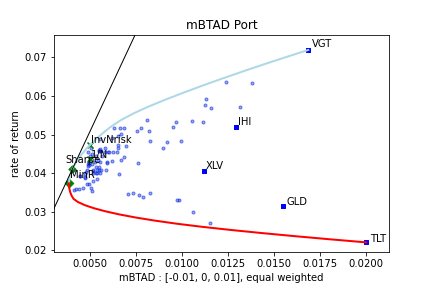
\includegraphics[width=.95\linewidth]{../figs/mBTADFrontier1.png}
  \caption{Rate of return vs. \mBTAD}
  \label{BTAD_fig1a}
\end{subfigure}%
\begin{subfigure}{.5\textwidth}
  \centering
  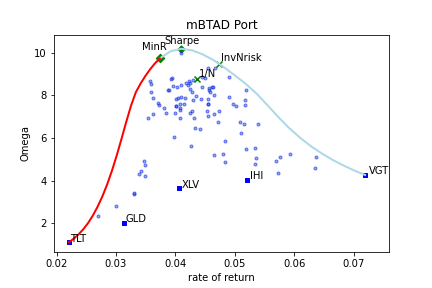
\includegraphics[width=.95\linewidth]{../figs/mBTADFrontier2.png}
  \caption{Omega vs. rate of return}
  \label{BTAD_fig1b}
\end{subfigure}
\caption{\mBTAD\ : [$\alpha=(-0.01, 0.0, 0.01)$, equal weighted] frontiers.}
\label{BTAD_fig1}
\end{figure}

\BackToContents

\subsubsection{Backtesting Omega optimal portfolio}

Here is an example, using \azapy\ package, of computing a portfolio backtesting.
For this example, we have chosen a portfolio quarterly rebalanced according
to the maximization of Omega ratio. At each rebalancing date,
the portfolio weights
are calibrated based on 3.25 years of prior historical market data.

Other rebalancing strategies can be considered
by changing the value of {\it rtype} parameter in the call of {\it set\_model} function below.
For more details see the package documentation at \azapydoc.

\lstinputlisting[language=Python]{../PyScripts/BTAD_Port.py}

\begin{figure}[H]
    \centering
    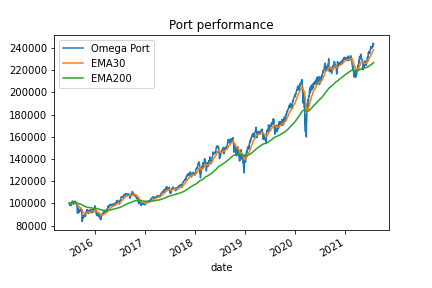
\includegraphics[width=.95\linewidth]{../figs/Port_mBTAD_Sharpe.png}
    \caption{Backtesting of quarterly rebalanced Omega optimal portfolio for
    \mBTAD\ : [$\alpha=(-0.01, 0.0, 0.01)$, equal weighted].}
    \label{BTAD_Port_fig}
\end{figure}


\BackToContents




\subsection{mBTSD-based optimization strategies}\label{S:mBTSD}

\BTSD\ stands for Below Threshold Semi-Deviation.
It is the square root of below threshold semi-variance proposed by Markowitz in 1959 \cite{Markowitz2}.
In contrast to standard deviation, \BTSD\ takes in account only the downside events below a prespecified threshold.

Its mathematical expression is given by $\BTM^{(p)}$, from Eq.~(\ref{btm1}), for $p=2$, \ie,
\begin{equation}
    \BTSD_\alpha = \left\| \left( \alpha - r \right)^+ \right\|_2,
    \label{btsd01}
\end{equation}
where $\alpha$ is the threshold level and $\|\cdot\|_2 = (\mE[|\cdot |^2])^{1/2}$ is the $L^2$-norm.
Note that \BTSD\ is the $L_2$ version of \BTAD.

\BTSD\ has gained more attention after the introduction of
Sortino ratio in 1994 by Sortino and Price \cite{Sortino} (see also \cite{Kaplan}).

Sortino ratio is defined as
\begin{equation}
    \Sortino_\alpha = \frac{\mE[r] - \alpha}{\BTSD_\alpha},
    \label{btsd02}
\end{equation}
and is equivalent to \BTSD-Sharpe ratio for $\mu_0 = \alpha$.
In contrast to the Sharpe ratio, Sortino ratio measures the expected excess returns 
per unit of downside risk of realizations below a predefined threshold.

As we mentioned in the preamble of this section, \BTSD\ can be defined in terms of both standard rate of return, $r$, and
detrended rate of return, $\br = r - \mE[r]$. In this subsection we will use the latter specification to express mathematical formulas.
However, we should keep in
mind that, switching between the \BTSD\ definitions, is a simple matter of replacing $\br$ with $r$.\footnote{The \azapy\ package provides a logical
flag to switch between the use of $r$ and $\br$ (see \azapydoc).}

Like \mBTAD\ from Eq.~(\ref{btm2}), \BTSD\ can be extended to a mixture, \ie,
\begin{equation}
    \mBTSD = \sum_{l=1}^L \cK_l \times \BTSD_{\alpha_l},
    \label{btsd0}
\end{equation}
where $\{\cK_l\}_{l=1,\cdots,L}$ is a set of positive coefficients normalized to unit (the mixture coefficients) and
$\{\alpha_l\}_{l=1,\cdots,L}$ is a set of distinct thresholds.

We will refer to the \mBTSD-Sharpe ratio as Sortino ratio since Sortino ratio terminology is more popular among practitioners. However,
we should keep in mind that our Sortino ratio definition is equivalent to the original Sortino and Price \cite{Sortino}
definition only in the case where $L=1$ and $\alpha_1 = \mu_0$ with standard rate of return.

Like \mBTAD, \mBTSD\ is not a genuine dispersion measure. It violates the positive homogeneity axiom and, in the case where standard rates of return
are used, it also violates local invariance. An exception is the case where $L=1$ and $\alpha_1=0$ with detrended rates of return.
In this case, $\BTSD_0$ is equivalent to the first order \mLSD, delta-risk $\delta^{(2)}_1$ from Eq.~(\ref{LSD02}), which is a genuine dispersion measure.

\BackToContents


\subsubsection{mBTSD dispersion measure}
The computation of \mBTSD\ is straightforward. Given a set $\{r_i\}_{i=1,\cdots,N}$ of observed rates or returns, we have
\begin{equation}
    \BTAD_\alpha = \left( \frac{1}{N}\sum_{i=1}^N \left[ \left(\alpha - \br_i \right)^+ \right]^2 \right)^{1/2}.
    \label{btsd1}
\end{equation}
Then, \mBTSD\ is given by the sum from Eq.~(\ref{btsd0}).

\BackToContents

\subsubsection{mBTSD optimal portfolio}
The optimization is described by Eqs.~(\ref{gg1}) from Sec.~\ref{strategies} point~\ref{OptRisk},
where $\rho$ is given by $\mBTSD$ from Eq.~(\ref{btsd0}).
It is the following SOCP problem.

\bigskip
\noindent Minimize over $\{\{w_k\}_{k=1,\cdots,M}, \{ \eta_l, \{ s_{li} \}_{i=1,\cdots,N} \}_{l=1,\cdots,L} \}$,
\begin{subequations}\label{btsd2}
\begin{align}
    &g = \sum_{l=1}^L \cK_l \eta_l, \label{btsd2a} \\
    \st &\left( \frac{1}{N} \sum_{i=1}^N s_{li}^2 \right)^{1/2} \leq \eta_l, \label{btsd2b} \\
    & s_{li} + \sum_{k=1}^M w_k \br_{ki} \geq \alpha_l, \label{btsd2c} \\
    & \sum_{k=1}^M w_k \mu_k \geq \mu, \label{btsd2d} \\
    & \sum_{k=1}^M w_k = 1, \label{btsd2e} \\
    & s_{li} \geq 0, \label{btsd2g} \\
    & \eta_l \geq 0, \label{btsdg} \\
    & w_k \geq 0, \label{btsd2f}
\end{align}
\end{subequations}

\noindent where $\mu$, in Eq.~(\ref{btsd2d}), is the portfolio targeted expected rate of return, while $\mu_k$ for $k = 1,\cdots,M$
are the portfolio components expected rate of returns.
Then, we have
\begin{subequations}\label{btsd3}
\begin{align}
    \RR &= \sum_{k=1}^M w_k^* \mu_k, \label{btsd3a} \\
    \mBTSD &= g^*, \label{btsd13b} \\
    \BTSD_{\alpha_l} &= \eta_l^*, \label{btsd3c}
\end{align}
\end{subequations}

\noindent where $^*$ denotes the solution of  SOCP problem.
In addition to the optimal portfolio weights $\{w_k^*\}_{k=1,\cdots,M}$ and
expected rate of return $\RR$, the
SOCP solution provides information about the portfolio \mBTSD\ and its components.

\bigskip
\noindent Here is an example, using the \azapy\ package, of how to compute the \mBTSD\ optimal portfolio.
The \mBTSD\ time horizon was set to one quarter and the calibration is performed using the prior 3.25 years of
close-adjusted historical prices (default settings).
For more details see the package documentation at \azapydoc.

\lstinputlisting[language=Python]{../PyScripts/BTSD_RiskOptim.py}

\BackToContents


\subsubsection{Minimum mBTSD portfolio}

Following the result from Sec.~\ref{strategies} point~\ref{MinRisk},
the algorithm to compute the optimal portfolio with minimum \mBTSD\ is given by Eqs.~(\ref{btsd1}) where
$\mu$ from r.h.s. of Eq.~(\ref{btsd2d}) is set to a value equal to the smallest expected rate of
return among the portfolio components, \ie\ $\mu=\min_k\{\mu_k\}$.

\bigskip
\noindent Here is an example, using the \azapy\ package, of how to compute the minimum \mBTSD\ portfolio.
The \mBTSD\ time horizon was set to one quarter and the calibration is performed using the prior 3.25 years of
close-adjusted historical prices (default settings).
For more details see the package documentation at \azapydoc.

\lstinputlisting[language=Python]{../PyScripts/BTSD_MinRisk.py}

\BackToContents


\subsubsection{mBTSD optimal portfolio for targeted risk value}
This optimization is described by Eqs.~(\ref{gg2}) from Sec.~\ref{strategies} point~\ref{TargetRisk},
where $\rho$ is given by \mBTSD\ from Eq.\ (\ref{btsd0}).
It is the following SOCP problem.

\bigskip
\noindent Maximize over $\{\{w_k\}_{k=1,\cdots,M}, \{ \eta_l, \{ s_{li} \}_{i=1,\cdots,N} \}_{l=1,\cdots,L} \}$,
\begin{subequations}\label{btsd4}
\begin{align}
    &g = \sum_{k=1}^M w_k \mu_k, \label{btsd4a} \\
    \st & \left( \frac{1}{N}  \sum_{i=1}^N s_{li}^2 \right)^{1/2} \leq \eta_l, \label{btsd4c} \\
    & s_{li} + \sum_{k=1}^M w_k \br_{ki} \geq \alpha_l, \label{btsd4d} \\
    & \sum_{l=1}^L \cK_l \eta_l = \mBTSD_0, \label{btsd4b} \\
    & \sum_{k=1}^M w_k = 1, \label{btsd4e} \\
    & s_{li} \geq 0, \label{btsd4g} \\
    & \eta_l \geq 0, \label{btsd4h} \\
    & w_k \geq 0, \label{btsd4f}
\end{align}
\end{subequations}

\noindent where $\mBTSD_0$ in Eq.~(\ref{btsd4b}) is the portfolio targeted \mBTSD\ dispersion value.
Then, we have
\begin{subequations}\label{btsd5}
\begin{align}
    \RR &= g^*, \label{btsd5a} \\
    \BTSD_{\alpha_l} &= \eta_l^*, \label{btsd5b}
\end{align}
\end{subequations}

\noindent where the superscript $^*$ denotes the solution of SOCP problem.
In addition to the optimal portfolio weights $\{w_k^*\}_{k=1,\cdots,M}$ and expected rate of return $\RR$,
the SOCP solution provides information about \mBTSD\ and its components,
although, this information is likely to be known at the outset.

\bigskip
\noindent Here is an example, using the \azapy\ package, of how to compute the optimal portfolio
with the same \mBTSD\ as the equal weighted portfolio.
The \mBTSD\ time horizon was set to one quarter and the calibration is performed using the prior 3.25 years of
close-adjusted historical prices (default settings).
For more details see the package documentation at \azapydoc.

\lstinputlisting[language=Python]{../PyScripts/BTSD_InvNrisk.py}

\BackToContents


\subsubsection{mBTSD optimal portfolio for fixed risk-aversion factor}
This optimization is described by Eqs.~(\ref{gg3}) from Sec.~\ref{strategies} point~\ref{RiskAverse},
where $\rho$ is given by \mBTSD\ from Eq.~(\ref{btsd0}).
It is the following LP problem.

\bigskip
\noindent Maximize over $\{\{w_k\}_{k=1,\cdots,M}, \{ \eta_l, \{ s_{li} \}_{i=1,\cdots,N} \}_{l=1,\cdots,L} \}$,
\begin{subequations}\label{btsd6}
\begin{align}
    &g = \sum_{k=1}^M w_k \mu_k - \lambda \sum_{l=1}^L \cK_l \eta_l, \label{btsd6a} \\
    \st & \left( \frac{1}{N}  \sum_{i=1}^N s_{li}^2 \right)^{1/2} \leq \eta_l, \label{btsd6b} \\
    & s_{li} + \sum_{k=1}^M w_k \br_{ki} \geq \alpha_l, \label{btsd6c} \\
    & \sum_{k=1}^M w_k = 1, \label{btsd6d} \\
    & s_{li} \geq 0, \label{btsd6f} \\
    & \eta_l \geq 0, \label{btsd6g} \\
    & w_k \geq 0, \label{btsd6e}
\end{align}
\end{subequations}

\noindent where $\lambda$ from Eqs.~(\ref{btsd6a}) is the risk-aversion factor.
Then, we have
\begin{subequations}\label{btsd7}
\begin{align}
    \RR &= \sum_{k=1}^M w_k^* \mu_k, \label{btsd7a} \\
    \mBTSD &= \frac{\RR - g^*}{\lambda}, \label{btsd7b} \\
    \BTSD_{\alpha_l} &= \eta_l^*, \label{btsd7c}
\end{align}
\end{subequations}

\noindent where the superscript $^*$ denotes the solution of SOCP problem.
In addition to the optimal portfolio weights $\{w_k^*\}_{k=1,\cdots,M}$ and expected rate of return $\RR$,
the SOCP solution provides information about \mBTSD\ and its \BTSD\ components values.

\bigskip
\noindent Here is an example, using the \azapy\ package, of how to compute the optimal portfolio
for a given value of the risk-aversion factor $\lambda$.
The \mBTSD\ time horizon was set to one quarter and the calibration is performed using the prior 3.25 years of
close-adjusted historical prices (default settings).
For more details see the package documentation at \azapydoc.

\lstinputlisting[language=Python]{../PyScripts/BTSD_Averse.py}

\BackToContents


\subsubsection{Sortino optimal portfolio - maximization solution}
This optimization targets the maximization of Sortino ratio. It is based on the
Eqs.~(\ref{gg4}) from Sec.~\ref{strategies} point~\ref{MaxSharpe}, where $\rho$ is given by \mBTSD\ from Eq.~(\ref{btsd0}).
The optimization can be formulated as an SOCP problem
if Eq.\ (\ref{gg4b}) can be expressed as a second order cone constraint. This can be achieved by
introducing the variable transformations $\bw_k = t w_k$, $\bs_{li} = t s_{li}$ and $\bbeta_l = t \eta_l$.
Then, the SCOP problem can be written as follows.

\bigskip
\noindent Maximize over $\{\{\bw_k\}_{k=1,\cdots,M}, \{ \bbeta_l, \{ \bs_{li} \}_{i=1,\cdots,N} \}_{l=1,\cdots,L}, t \}$,
\begin{subequations}\label{btsd8}
\begin{align}
    &g = \sum_{k=1}^M \bw_k \mu_k - \mu_0 t, \label{btsd8a} \\
    \st &\left( \frac{1}{N}  \sum_{i=1}^N \bs_{li}^2 \right)^{1/2} \leq \bbeta_l, \label{btsd8c} \\
    &\bs_{li}  + \sum_{k=1}^M \bw_k \br_{ki} - \alpha_l t \geq 0, \label{btsd8d} \\
    &\sum_{l=1}^L \cK_l \bbeta_l = 1, \label{btsd8b} \\
    &\sum_{k=1}^M \bw_k - t = 0, \label{btsd8e} \\
    &t \geq 0, \label{btsd8h} \\
    &\bs_{li} \geq 0, \label{btsd8g} \\
    &\bbeta_l \geq 0, \label{btsd8i} \\
    &\bw_k \geq 0, \label{btsd8f}
\end{align}
\end{subequations}

\noindent where $\mu_0$ in Eqs.~(\ref{btsd8a}) is the
risk-free rate accessible to the investor.
Then, we have
\begin{subequations}\label{btsd9}
\begin{align}
    w_k &= \frac{\bw_k^*}{t^*} , \label{btsd9a} \\
    \RR &= \frac{g^*}{t^*} + \mu_0, \label{btsd9c} \\
    \Sortino &= g^*, \label{btsd9b} \\
    \mBTSD &= \frac{1}{t^*}, \label{btsd9d} \\
    \BTSD_{\alpha_l} &= \frac{\bbeta_l^*}{t^*}, \label{btsd9e}
\end{align}
\end{subequations}

\noindent where $^*$ denotes the solution of SOCP problem.
In addition to the optimal portfolio weights $\{w_k\}_{k=1,\cdots,M}$, expected rate of return $\RR$ and
Sortino ratio $\Sortino$,
the SOCP solution provides information about \mBTSD\ and its components.

\bigskip
\noindent Here is an example, using the \azapy\ package, of how to compute the Sortino optimal portfolio using the maximization
of Sortino ratio.
The \mBTSD\ time horizon was set to one quarter and the calibration is performed using the prior 3.25 years of
close-adjusted historical prices (default settings).
For more details see the package documentation at \azapydoc.

\lstinputlisting[language=Python]{../PyScripts/BTSD_Sharpe.py}

\BackToContents


\subsubsection{Sortino optimal portfolio - minimization solution}
This optimization targets the minimization of the inverse of Sortino ratio.
It is described by Eqs.~(\ref{gg8}) from Sec.~\ref{strategies} point~\ref{MinSharpe}, where
$\rho$ is given by \mBTSD\ from Eq.~(\ref{btsd0}).
The optimization can be formulated as an SOCP problem if Eq.~(\ref{gg8a}) can  be expressed as a second order cone constraint. This can be achieved by
introducing the variable transformations
$\bw_k = t w_k$, $\bs_{li} = t s_{li}$ and $\bbeta_l = t \eta_l$.
Then, the SOCP problem can be written as follows.

\bigskip
\noindent Minimize over $\{ \{\bw_k\}_{k=1,\cdots,M}, \{ \bbeta_l, \{ \bs_{li} \}_{i=1,\cdots,N} \}_{l=1,\cdots,L}, t \}$
\begin{subequations}\label{btsd10}
\begin{align}
    &g = \sum_{l=1}^L \cK_l \bbeta_l, \label{btsd10a} \\
    \st &\left( \frac{1}{N}  \sum_{i=1}^N \bs_{li}^2 \right)^{1/2} \leq \bbeta_l, \label{btsd10b} \\
    &\bs_{li}  + \sum_{k=1}^M \bw_k \br_{ki} - \alpha_l t \geq 0, \label{btsd10c} \\
    &\sum_{k=1}^M \bw_k \mu_k -\mu_0 t = 1, \label{btsd10d} \\
    &\sum_{k=1}^M \bw_k - t = 0, \label{btsd10e} \\
    &t \geq 0, \label{btsd10h} \\
    &\bs_{li} \geq 0, \label{btsd10g} \\
    &\bbeta_l \geq 0, \label{btsd10i} \\
    &\bw_k \geq 0, \label{btsd10f}
\end{align}
\end{subequations}

\noindent where $\mu_0$ in Eqs.~(\ref{btsd8a}) is the
risk-free rate accessible to the investor.
Then, we have
\begin{subequations}\label{btsd11}
\begin{align}
    w_k &= \frac{\bw_k^*}{t^*} , \label{btsd11a} \\
    \RR &= \frac{1}{t^*} + \mu_0, \label{btsd11c} \\
    \Sortino &= \frac{1}{g^*}, \label{btsd11b} \\
    \mBTSD &= \frac{g^*}{t^*}, \label{btsd11d} \\
    \BTSD_{\alpha_l} &= \frac{\bbeta_l^*}{t^*}, \label{btsd11e}
\end{align}
\end{subequations}

\noindent where $^*$ denotes the solution of SOCP problem.
In addition to the optimal portfolio weights $\{w_k\}_{k=1,\cdots,M}$, expected rate of return $\RR$ and
Sortino ratio \Sortino,
the SOCP solution provides information about \mBTSD\ and its \BTSD\ components.

\bigskip
\noindent Here is an example, using the \azapy\ package, of how to compute the Sortino optimal portfolio using the minimization
of the inverse of Sortino ratio.
The \mBTSD\ time horizon was set to one quarter and the calibration is performed using the prior 3.25 years of
close-adjusted historical prices (default settings).
For more details see the package documentation at \azapydoc.

\lstinputlisting[language=Python]{../PyScripts/BTSD_InvSharpe.py}

\BackToContents


\subsubsection{mBTSD frontiers}

Here is an example of how to compute the \mBTSD\ frontiers using the \azapy\
package. The \mBTSD\ time horizon was set to one quarter and the calibration is performed using the prior 3.25 years of
close-adjusted historical prices (default settings).
For more details see the package documentation at \azapydoc.

The script will produce the plots in Figs.~\ref{BTSD_fig1a} and \ref{BTSD_fig1b}
for historical data collected up to 2021-07-27.

\lstinputlisting[language=Python]{../PyScripts/BTSD_frontiers.py}

\begin{figure}[H]
\centering
\begin{subfigure}{.5\textwidth}
  \centering
  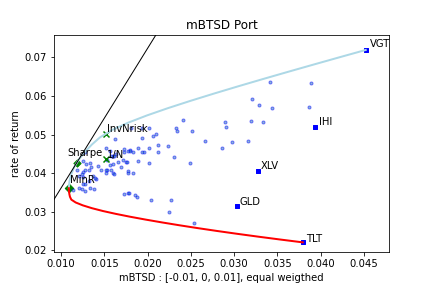
\includegraphics[width=.95\linewidth]{../figs/mBTSDFrontier1.png}
  \caption{Rate of return vs. \mBTSD}
  \label{BTSD_fig1a}
\end{subfigure}%
\begin{subfigure}{.5\textwidth}
  \centering
  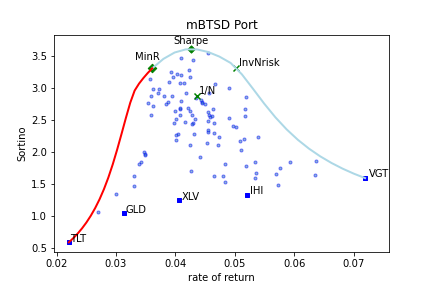
\includegraphics[width=.95\linewidth]{../figs/mBTSDFrontier2.png}
  \caption{Sortino vs. rate of return}
  \label{BTSD_fig1b}
\end{subfigure}
\caption{\mBTSD\ : [$\alpha=(-0.01, 0.0, 0.01)$, equal weighted] frontiers.}
\label{BTSD_fig1}
\end{figure}

\BackToContents


\subsubsection{Backtesting Sortino optimal portfolio}

Here is an example, using \azapy\ package, of computing a portfolio backtesting.
For this example, we have chosen a portfolio quarterly rebalanced according
to the maximization of Sortino ratio. At each rebalancing date,
the portfolio weights
are calibrated based on 3.25 years of prior historical market data.

Other rebalancing strategies can be considered
by changing the value of {\it rtype} parameter in the call of {\it set\_model} function below.
For more details see the package documentation at \azapydoc.

\lstinputlisting[language=Python]{../PyScripts/BTSD_Port.py}

\begin{figure}[H]
    \centering
    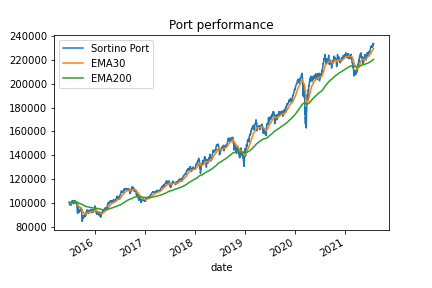
\includegraphics[width=.95\linewidth]{../figs/Port_mBTSD_Sharpe.png}
    \caption{Backtesting of quarterly rebalanced Sortino optimal portfolio,
    \mBTSD\ : [$\alpha=(-0.01, 0.0, 0.01)$, equal weighted].}
    \label{BTSD_Port_fig}
\end{figure}

\BackToContents
 

\section{Inter-observations distance measures}
The inter-observations distance measure can be expressed  as
\begin{equation}
    \HMOD^{(p)}(X) = \frac{1}{2^{1/p}}\left\| Y - Z \right\|_p,
    \label{hmod1}
\end{equation}
where \HMOD\ stands for Higher Moment inter-Observations Distance,
$\|\cdot\|_p = (\mE[|\cdot|^p])^{1/p}$ is the $L^p$-norm, and
$Y$ and $Z$ are two \iid copies of $X$.

$\HMOD^{(p)}$ are genuine dispersion measures. Further, they can
be classified as symmetric dispersion measures, in the sense that they do not provide an excess penalty to downside events.

Given a set of  historical observations $\{r_i\}_{i=1,\cdots,N}$, Eq.~(\ref{hmod1}) can be approximated by
\begin{equation}
    \HMOD^{(p)} = \frac{1}{N^{2/p}}\left( \sum_{i=1}^{N-1} \sum_{j=i+1}^N \left|r_i - r_j \right|^p \right)^{1/p}.
    \label{hmod2}
\end{equation}
From a numerical point of view, the \HMOD-based portfolio optimizations pose a unique challenge. Since they are expressed in terms of pairwise
observations, the computation effort tends to scale up quadratic in the number of historical observations.

A famous member of this family is for $p=1$, the \GINI\
dispersion measure. Historically, it was inspired by the \GINI\ index from
sociology formulated by Corrado Gini in 1912 (see \cite{Giorgi}). It was introduced to finance in 1982 by Yitzhaki \cite{Yitzhaki}.
Portfolio optimizations strategies based on the \GINI\ dispersion measure will be presented in the next subsection.

For $p=2$ we have another famous dispersion measure. In this case $\HMOD^{(2)}$ reduces to the standard deviation, \SD, \ie,
\begin{equation}
    \HMOD^{(2)}(X) = \std(X),
    \label{hmod3}
\end{equation}
where $\std(\cdot)$ is the standard deviation operator.

The \SD\ optimal portfolio strategies can be expressed in terms of the covariance matrix between the portfolio components,
avoiding an explicit pairwise formulation at the SOCP level.
The computation complexity becomes quadratic in the number of portfolio components rather than in the number of historical observations.
In this sense, $\HMOD^{(2)}$ is an exception among the \HMOD\ dispersion measures. This class of optimal portfolio
strategies are presented in Sec.~\ref{S:SD}.

\BackToContents


\subsection{Gini-based optimization strategies}\label{S:GINI}


\subsubsection{Gini dispersion measure}
As we mentioned, \GINI\ dispersion measure is given by Eq.~(\ref{hmod2}) for $p=1$, \ie,
\begin{equation}
    \GINI = \frac{1}{N^2}\sum_{i=1}^{N-1}\sum_{j=i+1}^N \left| r_i - r_j \right|,
    \label{gini0}
\end{equation}
where $r_i$ is the rate of return $i$-th historical observation.

Numerically, \GINI\ measure can be evaluated directly using Eq.~(\ref{gini0}). However, the computation can be
speed up significantly by transforming the double sum in a single sum.

Let $\{x_i\}_{i=1,\cdots,N}$ be $\{r_i\}_{i=1,\cdots,N}$ sorted in ascending order. Then, after some straightforward
algebraic manipulations, Eq.~(\ref{gini0}) can be rewritten as
\begin{equation}
    \GINI = \frac{1}{N^2}\sum_{i=1}^N (2 i - N  + 1) x_i.
    \label{gini00}
\end{equation}
A computation algorithm based on
Eq.~(\ref{gini00}), assuming a heapsort algorithm followed by a single sum, has a complexity of $\cO(N \log(N))$,
while an algorithm based on Eq.~(\ref{gini0}), involving a double sum, has a complexity of $\cO(N^2)$, where $N$ is
the number of observations.\footnote{As a guideline, a typical value for $N$ is $1,000$.}
Therefore, the evaluation of \GINI\ based on Eq.~(\ref{gini00}) is faster.
This approach has been implemented in the \azapy\ package.

\BackToContents

\subsubsection{Gini optimal portfolio}
This optimization is described by Eqs.~(\ref{gg1}) from Sec~\ref{strategies} point~\ref{OptRisk},
where $\rho$ is given by \GINI\ from Eq.\ (\ref{gini0}).
It is the following LP problem.

\bigskip
\noindent Minimize over $\{ \{w_k\}_{k=1,\cdots,M}, \{s_{ij}\}_{i=1,\cdots,N-1; j = i+1,\cdots,N} \}$
\begin{subequations}\label{gini1}
\begin{align}
    &g = \frac{1}{N^2} \sum_{i=1}^{N-1} \sum_{j = i+1}^N s_{ij}, \label{gini1a} \\
    \st &s_{ij} \geq \sum_{k=1}^M w_k (r_{ki} - r_{kj}), \label{gini1b} \\
        &s_{ij} \geq -\sum_{k=1}^M w_k (r_{ki} - r_{kj}), \label{gini1c} \\
        &\sum_{k=1}^M w_k \mu_k \geq \mu, \label{gini1d} \\
        & \sum_{k=1}^M w_k = 1, \label{gini1e} \\
        & s_{ij} \geq 0, \label{gini1g} \\
        & w_k \geq 0, \label{gini1f}
\end{align}
\end{subequations}

\noindent where $\mu$ in Eq.~(\ref{gini1d}) is the portfolio targeted rate of return while $\{\mu_k\}_{i=1,\cdots,M}$
are the portfolio components expected rate of returns.
Then, we have
\begin{subequations}\label{gini2}
\begin{align}
    \RR &= \sum_{k=1}^M w_k^* \mu_k, \label{gini2a} \\
    \GINI &= g^*, \label{gini2b}
\end{align}
\end{subequations}

\noindent where $^*$ denotes the solution of LP problem.
In addition to the portfolio weights $\{w_k^*\}_{k=1,\cdots,M}$ and expected rate of return $\RR$, the
LP solution provides information about the portfolio \GINI\ dispersion.

The number of variables in the LP from Eqs.\ (\ref{gini1}) is $M + N(N-1)/2$. It scales quadratic with the number
of historical observations, $N$.
This rapid grow of dimensionality, leading to excessive computational efforts, is the main disadvantage of any \GINI-based optimal portfolio
strategy evaluation. However, keeping the length of historical observation at reasonable values (say, 1-2 year) the \GINI-based
optimization strategies are numerically tractable.

\bigskip
\noindent Here is an example, using the \azapy\ package, of how to compute the \GINI\ optimal portfolio.
The \GINI\ time horizon was set to one quarter and the calibration is performed using 1.25 years of
close-adjusted historical prices (default settings).
For more details see the package documentation at \azapydoc.

\lstinputlisting[language=Python]{../PyScripts/Gini_RiskOptim.py}

\BackToContents


\subsubsection{Minimum Gini portfolio}

Following the results from Sec.~\ref{strategies} point~\ref{MinRisk},
the algorithm to compute the optimal portfolio with minimum \GINI\ dispersion is given by the LP problem from Eqs.~(\ref{gini1}) where
$\mu$ from r.h.s. of Eq.~(\ref{gini1d}) is set to a value equal to the smallest expected rate of
return among the portfolio components, \ie\ $\mu=\min_k\{\mu_k\}$.

\bigskip
\noindent Here is an example, using the \azapy\ package, of how to compute the minimum \GINI\ portfolio.
The \GINI\ time horizon was set to one quarter and the calibration is performed using 1.25 years of
close-adjusted historical prices (default settings).
For more details see the package documentation at \azapydoc.

\lstinputlisting[language=Python]{../PyScripts/Gini_MinRisk.py}

\BackToContents


\subsubsection{Gini optimal portfolio for targeted risk value}
This optimization is described by  Eqs.~(\ref{gg2}) from Sec~\ref{strategies} point~\ref{MinRisk},
where $\rho$ is given by \GINI\ from Eq.~(\ref{gini0}).
It is the following LP problem.

\bigskip
\noindent Maximize over $\{ \{w_k\}_{k=1,\cdots,M}, \{s_{ij}\}_{i=1,\cdots,N-1; j = i+1,\cdots,N} \}$
\begin{subequations}\label{gini3}
\begin{align}
    &g = \sum_{k=1}^M w_k \mu_k , \label{gini3a} \\
    \st & \frac{1}{N^2} \sum_{i=1}^{N-1} \sum_{j = i+1}^N s_{ij} = \GINI_0, \label{gini3d} \\
        & s_{ij} \geq \sum_{k=1}^M w_k (r_{ki} - r_{kj}), \label{gini3b} \\
        & s_{ij} \geq -\sum_{k=1}^M w_k (r_{ki} - r_{kj}), \label{gin3c} \\
        & \sum_{k=1}^M w_k = 1, \label{gini3e} \\
        & s_{ij} \geq 0, \label{gini3g} \\
        & w_k \geq 0, \label{gin3f}
\end{align}
\end{subequations}

\noindent where $\GINI_0$ from Eq.~(\ref{gini3d}) is the targeted portfolio \GINI\ dispersion value.
Then, the portfolio expected rate of return is given by the value of the objective
function, \ie,
\begin{equation}
    \RR = g^*, \label{gini4}
\end{equation}

\noindent and the optimal portfolio weights by $\{w^*_k\}_{k=1,\cdots,M}$. The superscript $^*$ denotes the
solution of LP problem.

\bigskip
\noindent Here is an example, using the \azapy\ package, of how to compute the optimal portfolio
with the same \GINI\ as the equal weighted portfolio.
The \GINI\ time horizon was set to one quarter and the calibration is performed using 1.25 years of
close-adjusted historical prices (default settings).
For more details see the package documentation at \azapydoc.

\lstinputlisting[language=Python]{../PyScripts/Gini_InvNrisk.py}

\BackToContents


\subsubsection{Gini optimal portfolio for fixed risk-aversion factor}
This optimization is described by Eqs.\ (\ref{gg3}) from Sec~\ref{strategies} point~\ref{MinRisk},
where $\rho$ is given by \GINI\ from Eq.\ (\ref{gini0}).
It is the following LP problem.

\bigskip
\noindent Maximize over $\{ \{w_k\}_{k=1,\cdots,M}, \{s_{ij}\}_{i=1,\cdots,N-1; j = i+1,\cdots,N} \}$
\begin{subequations}\label{gini5}
\begin{align}
    &g = \sum_{k=1}^M w_k \mu_k - \frac{\lambda}{N^2} \sum_{i=1}^{N-1} \sum_{j = i+1}^N s_{ij}, \label{gini5a} \\
    \st &s_{ij} \geq \sum_{k=1}^M w_k (r_{ki} - r_{kj}), \label{gini5b} \\
        &s_{ij} \geq -\sum_{k=1}^M w_k (r_{ki} - r_{kj}), \label{gini5c} \\
        & \sum_{k=1}^M w_k = 1, \label{gini5d} \\
        & s_{ij} \geq 0, \label{gini5f} \\
        & w_k \geq 0, \label{gini5e}
\end{align}
\end{subequations}

\noindent where $\lambda$ in Eq.\ (\ref{gini5a}) is the risk aversion coefficients.
Then, we have
\begin{subequations}\label{gini6}
\begin{align}
    \RR &= \sum_{k=1}^M w_k^* \mu_k, \label{gini6a} \\
    \GINI &= \frac{\RR - g^*}{\lambda}, \label{gini6b}
\end{align}
\end{subequations}

\noindent where $^*$ denotes the solution of LP problem.
In addition to the portfolio weights $\{w_k^*\}_{k=1,\cdots,M}$, the
LP solution provides information about the portfolio \GINI\ dispersion.

\bigskip
\noindent Here is an example, using the \azapy\ package, of how to compute the optimal portfolio
for a given value of the risk aversion coefficient $\lambda$.
The \GINI\ time horizon was set to one quarter and the calibration is performed using 1.25 years of
close-adjusted historical prices (default settings).
For more details see the package documentation at \azapydoc.

\lstinputlisting[language=Python]{../PyScripts/Gini_Averse.py}

\BackToContents


\subsubsection{Gini-Sharpe optimal portfolio - maximization solution}
This optimization targets the maximization of \GINI-Sharpe ratio. It is based on the
Eqs.~(\ref{gg4}) from Sec~\ref{strategies} point~\ref{MinRisk},
where $\rho$ is given by \GINI\ from Eq.~(\ref{gini0}).
The optimization can be formulated as an LP problem
if Eq.~(\ref{gg4b}) can be linearized. In our case the linearization is straightforward. Introducing the
variable transformations $\bw_k = t w_k$ and $\bs_{li} = t s_{li}$, the LP
problem can be written as follows.

\bigskip
\noindent Maximize over $\{ \{\bw_k\}_{k=1,\cdots,M}, \{\bs_{ij}\}_{i=1,\cdots,N-1; j = i+1,\cdots,N}, t \}$
\begin{subequations}\label{gini7}
\begin{align}
    &g = \sum_{k=1}^M \bw_k \mu_k - \mu_0 t, \label{gini7a} \\
    \st &\frac{1}{N^2} \sum_{i=1}^{N-1} \sum_{j=i+1}^N \bs_{ij} = 1, \label{gini7d} \\
        &\bs_{ij} \geq \sum_{k=1}^M \bw_k (r_{ki} - r_{kj}), \label{gini7b} \\
        &\bs_{ij} \geq -\sum_{k=1}^M \bw_k (r_{ki} - r_{kj}), \label{gini7c} \\
        & \sum_{k=1}^M \bw_k - t = 0, \label{gini7e} \\
        & t \geq 0, \label{gini7h} \\
        & \bs_{ij} \geq 0, \label{gini7g} \\
        & \bw_k \geq 0, \label{gini7f}
\end{align}
\end{subequations}


\noindent where $\mu_0$ in Eq.~(\ref{gini7a}) is the
risk-free rate accessible to the investor.
Then, we have
\begin{subequations}\label{gini8}
\begin{align}
    w_k &= \frac{\bw_k^*}{t^*} , \label{gini8a} \\
    \RR &= \frac{g^*}{t^*} + \mu_0, \label{gini8c} \\
    \Sharpe &= g^*, \label{gini8b} \\
    \GINI &= \frac{1}{t^*}, \label{gini8d}
\end{align}
\end{subequations}

\noindent where $^*$ denotes the solution of LP problem.
In addition to the optimal portfolio weights $\{w_k\}_{k=1,\cdots,M}$, expected rate of return $\RR$ and
\GINI-Sharpe ratio $\Sharpe$,
the LP solution provides information about the portfolio \GINI\ dispersion.

\bigskip
\noindent Here is an example, using the \azapy\ package, of how to compute the \GINI-Sharpe optimal portfolio using the maximization
of \GINI-Sharpe ratio.
The \GINI\ time horizon was set to one quarter and the calibration is performed using 1.25 years of
close-adjusted historical prices (default settings).
For more details see the package documentation at \azapydoc.

\lstinputlisting[language=Python]{../PyScripts/Gini_Sharpe.py}

\BackToContents


\subsubsection{Gini-Sharpe optimal portfolio - minimization solution}
This optimization targets the minimization of the inverse of \GINI-Sharpe ratio.
It is  described by Eqs.~(\ref{gg8}) from Sec.~\ref{strategies} point~\ref{MinSharpe}, where
$\rho$ is given by \GINI\ from Eq.~(\ref{gini0}).
The optimization can be formulated as an LP problem if Eq.~(\ref{gg8a}) can be linearized. This can be achieved by
introducing the variable transformations
$\bw_k = t w_k$ and $\bs_{li} = t s_{li}$.
Then, the LP problem can be written as follows.

\bigskip
\noindent Minimize over $\{ \{\bw_k\}_{k=1,\cdots,M}, \{\bs_{ij}\}_{i=1,\cdots,N-1; j = i+1,\cdots,N}, t \}$
\begin{subequations}\label{gini9}
\begin{align}
    &g = \frac{1}{N^2} \sum_{i=1}^{N-1} \sum_{j=i+1}^N \bs_{ij}, \label{gini9a} \\
    \st & \sum_{k=1}^M \bw_k\mu_k - \mu_0 t = 1, \label{gini9d} \\
        &\bs_{ij} \geq \sum_{k=1}^M \bw_k (r_{ki} - r_{kj}), \label{gini9b} \\
        &\bs_{ij} \geq -\sum_{k=1}^M \bw_k (r_{ki} - r_{kj}), \label{gini9c} \\
        & \sum_{k=1}^M \bw_k - t = 0, \label{gini9e} \\
        & t \geq 0, \label{gini9g} \\
        & \bs_{ij} \geq 0, \label{gini9h} \\
        & \bw_k \geq 0, \label{gini9f}
\end{align}
\end{subequations}

\noindent where $\mu_0$ in Eq.~(\ref{gini9d}) is the risk-free rate accessible to the investor.
Then we have,
\begin{subequations}\label{gini10}
\begin{align}
    w_k &= \frac{\bw_k^*}{t^*} , \label{gini10a} \\
    \RR &= \frac{1}{t^*} + \mu_0, \label{gini10c} \\
    \Sharpe &= \frac{1}{g^*}, \label{gini10b} \\
    \GINI &= \frac{g^*}{t^*}, \label{gini10d}
\end{align}
\end{subequations}

\noindent where $^*$ denotes the solution of LP problem.
In addition to the optimal portfolio weights $\{w_k\}_{k=1,\cdots,M}$, expected rate of return $\RR$ and
\GINI-Sharpe ratio $\Sharpe$,
the LP solution provides information about the portfolio \GINI\ dispersion.


\bigskip
\noindent Here is an example, using the \azapy\ package, of how to compute the \GINI-Sharpe optimal portfolio using the minimization
of the inverse of \GINI-Sharpe ratio.
The \GINI\ time horizon was set to one quarter and the calibration is performed using 1.25 years of
close-adjusted historical prices (default settings).
For more details see the package documentation at \azapydoc.

\lstinputlisting[language=Python]{../PyScripts/Gini_InvSharpe.py}

\BackToContents


\subsubsection{Gini frontiers}

Here is an example of how to compute the \GINI\ frontiers using the \azapy\
package. The \GINI\ time horizon was set to one quarter and the calibration is performed using 1.25 years of
close-adjusted historical prices (default settings).
For more details see the package documentation at \azapydoc.

The script produces the plots in Figs. \ref{GINI_fig1a} and \ref{GINI_fig1b}
for historical data collected up to 2021-07-27.

\lstinputlisting[language=Python]{../PyScripts/Gini_frontiers.py}

\begin{figure}[H]
\centering
\begin{subfigure}{.5\textwidth}
  \centering
  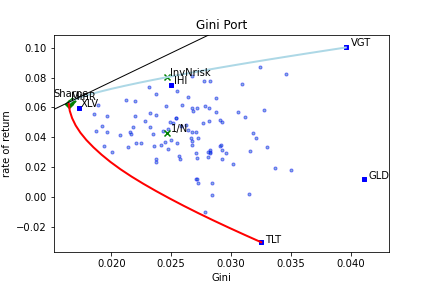
\includegraphics[width=.95\linewidth]{../figs/GINIFrontier1.png}
  \caption{Rate of return vs. \GINI}
  \label{GINI_fig1a}
\end{subfigure}%
\begin{subfigure}{.5\textwidth}
  \centering
  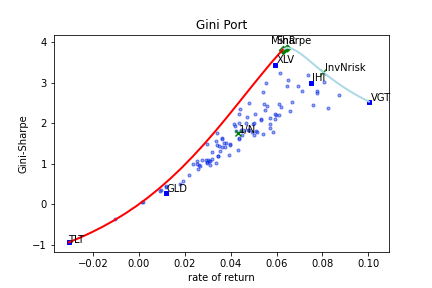
\includegraphics[width=.95\linewidth]{../figs/GINIFrontier2.png}
  \caption{\GINI-Sharpe vs. rate of return}
  \label{GINI_fig1b}
\end{subfigure}
\caption{\GINI\ frontiers.}
\label{GINI_fig1}
\end{figure}

\BackToContents

\subsubsection{Backtesting Gini-Sharpe optimal portfolio}

Here is an example, using \azapy\ package, of computing a portfolio backtesting.
For this example, we have chosen a portfolio quarterly rebalanced according
to the maximization of \GINI-Sharpe ratio. At each rebalancing date,
the portfolio weights
are calibrated based on 1.25 years of prior historical market data.

Other rebalancing strategies can be considered
by changing the value of {\it rtype} parameter in the call of {\it set\_model} function below.
For more details see the package documentation at \azapydoc.

\lstinputlisting[language=Python]{../PyScripts/Gini_Port.py}

\begin{figure}[H]
    \centering
    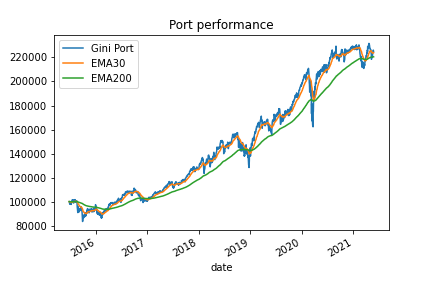
\includegraphics[width=.95\linewidth]{../figs/Port_GINI_Sharpe.png}
    \caption{Backtesting of quarterly rebalanced \GINI-Sharpe optimal portfolio.}
    \label{GINI_Port_fig}
\end{figure}

\BackToContents





\section{Central moment dispersion measures}\label{CentralM}
The central moment dispersion measures are defined as
\begin{equation}
    \CMDM^{(p)} = \left\| X - \mE[X] \right\|_p
    \label{cmdm1}
\end{equation}
where $\|\cdot\|_p = (\mE[|\cdot|^p])^{1/p}$ is the $L^p$-norm.
Note that $\CMDM^{(p)}$ is a genuine dispersion measure for any $p$.
In contrast to the tail, downside and below threshold measures, \CMDM\ are
symmetric. They do not provide an excess penalty to the downside
events.

For $p=1$ the \CMDM\ is equivalent to \MAD\ dispersion measure described in Sec.~\ref{S:mMAD}.

However, the most famous member of this family is for $p=2$, the standard deviation, \SD.
It is profoundly related to the 1952 Markowitz portfolio theory, \cite{Markowitz} and \cite{Markowitz2}.
In the original work, Markowitz had used the variance (the square of standard deviation) as a dispersion measure. Often the
variance based optimal portfolio strategies are called mean-variance, \MV.\footnote{Markowitz original terminology was E-V short
for expected rate of return vs. variance. These days, E-V terminology is rarely used, it was replaced by mean-variance, \MV.}
We will use the terminology {\it \MV-based optimal portfolio strategies} to designate portfolio strategies where variance is the dispersion measure.

Obviously, the \SD\ and \MV\ optimal portfolios are identical. Therefore, the \SD\ and \MV\
efficient frontiers are identical.\footnote{Two efficient frontiers are identical if and only if the composition of the portfolios
belonging to them are identical.} However, there are slight differences between the two measures.
Note that variance is not a genuine dispersion measure. It violates the positive homogeneity axiom. However, the formalism
of optimal portfolio strategies, outlined in Sec.~\ref{strategies}, holds. As we will see in the next two subsections,
the \SD\ and \MV\ optimization algorithms tend to be different.
\MV\ portfolio optimization is often described as a QP while \SD\ as an SOCP problem. However,
QP can be viewed as a special case of SOCP. In this sense the \SD\ and \MV\ optimal portfolio algorithms
could be regarded as similar.

Fundamental differences exist between the Sharpe type optimal portfolios.
The \SD-Sharpe ratio is the original Sharpe ratio introduced in 1966 by Sharpe in \cite{Sharpe1966} (see also \cite{Sharpe1994}).
For this reason, we will call \SD-Sharpe ratio simply as Sharpe ratio, preserving the original recognized terminology.
The \MV-Sharpe ratio is different than the Sharpe ratio. Therefore, Sharpe and \MV-Sharpe optimal portfolios are different.
However, since the \SD\ and \MV\ efficient frontiers are identical,
the \MV-Sharpe optimal portfolio belongs to the \SD\ efficient frontier and vice versa.

Similarly, the \SD\ and \MV\ optimal portfolios for the same risk-aversion factor value are different.
In fact, $\lambda_\SD$ (\SD-aversion factor) and $\lambda_\MV$ (\MV-aversion factor)
are two distinct parameterizations of the same efficient frontier.

The next two subsections present the \SD\ and \MV\ based optimal portfolio strategies algorithms separately.
We will point out along the way to the differences and similarities between the two approaches.
Overall, we prefer the \SD\ representation since it met all the scalability properties provided by a genuine
dispersion measure, especially for Sharpe optimal portfolios. However, the \MV\ representation is equally valid and
numerically robust.

\BackToContents


\subsection{SD-based optimization strategies}\label{S:SD}

\subsubsection{SD dispersion measure}

Standard deviation, \SD, is a special case, for $p=2$, of central momentum dispersion measure defined
in Eq.~(\ref{cmdm1}), \ie,
\begin{equation}
    \SD = \sqrt{\VAR(r)},
    \label{sd01}
\end{equation}
where $\VAR(r)$ is the variance of the rate of return. For a portfolio, defined by the set of weights $\{w_k\}_{k=1,\cdots,M}$,
Eq.~(\ref{sd01}) can be rewritten as
\begin{equation}
    \SD = \sqrt{w^T\cdot C\cdot w},
    \label{sd02}
\end{equation}
where $C$ is the covariance matrix between the portfolio components.
Although for direct computations either Eq.~(\ref{sd01}) or
Eq.~(\ref{sd0}) is sufficient, it is useful to mention the following alternative expression
\begin{equation}
    \SD = \| U\cdot w \|_2,
    \label{sd0}
\end{equation}
where $\|\cdot\|_2$ is the Euclidian norm and $U$ is a matrix such that $U^T\cdot U = C$. In general, $U$ is not unique.
If $C$ is a positive defined matrix, then $U$ can be given by the
Cholesky factorization. If $C$ is only positive semidefinite,\footnote{$C$ can be semidefinite if one of the portfolio components
is a risk-free asset (with zero volatility), \eg\ a pure cash position. \azapy\ implementation covers these cases too.} then $U$ can be computed as the
square root matrix.\footnote{The square root matrix of $C$ is the unique semidefinite matrix $U$ such that $U\cdot U = C$.}

\BackToContents


\subsubsection{SD optimal portfolio}
This optimization is described by Eqs.~(\ref{gg1}) from Sec~\ref{strategies} point~\ref{OptRisk},
where $\rho$ is given by \SD\ from Eq.\ (\ref{sd0}).
It is the following SOCP problem.

\bigskip
\noindent Minimize over $\{ \{w_k\}_{k=1,\cdots,M}, \eta \}$
\begin{subequations}\label{sd1}
\begin{align}
    & g = \eta, \label{sd1a} \\
    \st & \| U w \|_2 \leq \eta, \label{sd1b} \\
        & \sum_{k=1}^M w_k \mu_k \geq \mu_0, \label{sd1c} \\
        & \sum_{k=1}^K w_k = 1, \label{sd1d} \\
        & \eta \geq 0, \label{sd1f} \\
        & w_k \geq 0, \label{sd1e}
\end{align}
\end{subequations}

\noindent where $\mu$ from Eq.~(\ref{sd1c})
is the targeted portfolio rate of return, while $\mu_k$ for $k=1,\cdots,M$
are the portfolio components expected rate of returns.
Then, we have
\begin{subequations}\label{sd2}
\begin{align}
    \RR &= \sum_{k=1}^M w_k^* \mu_k, \label{sd2a} \\
    \SD &= g^*, \label{sd2b}
\end{align}
\end{subequations}

\noindent where $^*$ denotes the solution of SOCP problem.
In addition to the optimal portfolio weights $\{w_k^*\}_{k=1,\cdots,M}$ and expected
rate of return $\RR$, the
SOCP solution provides information about the portfolio standard deviation \SD.

\bigskip
\noindent Here is an example, using the \azapy\ package, of how to compute the \SD\ optimal portfolio.
The \SD\ time horizon was set to one quarter and the calibration is performed using 3.25 years of
close-adjusted historical prices (default settings).
For more details see the package documentation at \azapydoc.

\lstinputlisting[language=Python]{../PyScripts/SD_RiskOptim.py}

\BackToContents


\subsubsection{Minimum SD portfolio}

Following the results from Sec.~\ref{strategies} point~\ref{MinRisk},
the algorithm to compute the optimal portfolio with minimum \SD\ is given by the SOCP problem from Eqs.~(\ref{sd1}) where
$\mu$ from r.h.s. of Eq.~(\ref{sd1c}) is set to a value equal to the smallest expected rate of
return among the portfolio components, \ie\ $\mu=\min_k\{\mu_k\}$.

\bigskip
\noindent Here is an example, using the \azapy\ package, of how to compute the minimum \SD\ portfolio.
The \SD\ time horizon was set to one quarter and the calibration is performed using 3.25 years of
close-adjusted historical prices (default settings).
For more details see the package documentation at \azapydoc.

\lstinputlisting[language=Python]{../PyScripts/SD_MinRisk.py}

\BackToContents


\subsubsection{SD optimal portfolio for targeted risk value}
This optimization is described by Eqs.~(\ref{gg2}) from Sec.~\ref{strategies} point~\ref{TargetRisk},
where $\rho$ given by \SD\ from Eq.\ (\ref{sd0}).
It is the following SOCP problem.

\bigskip
\noindent Maximize over $\{ w_k \}_{k=1,\cdots, M}$
\begin{subequations}\label{sd3}
\begin{align}
    & g = \sum_{k=1}^M w_k \mu_k, \label{sd3a} \\
    \st & \| U w\|_2 \leq \SD_0, \label{sd3b} \\
        & \sum_{k=1}^M w_k = 1, \label{sd3c} \\
        & w_k \geq 0, \label{sd3d}
\end{align}
\end{subequations}

\noindent where $\SD_0$ from Eq.~(\ref{sd3b}) is the targeted portfolio \SD\ value.
The portfolio expected rate of return is given by the optimal value of the objective
function, \ie,
\begin{equation}
    \RR = g^*, \label{sd4}
\end{equation}

\noindent and the optimal portfolio weights by $\{w^*_k\}_{k=1,\cdots,M}$. The superscript $^*$ denotes the
solution of SOCP problem.


\bigskip
\noindent Here is an example, using the \azapy\ package, of how to compute the optimal portfolio
with the same \SD\ as the equal weighted portfolio.
The \SD\ time horizon was set to one quarter and the calibration is performed using 3.25 years of
close-adjusted historical prices (default settings).
For more details see the package documentation at \azapydoc.

\lstinputlisting[language=Python]{../PyScripts/SD_InvNrisk.py}

\BackToContents


\subsubsection{SD optimal portfolio for fixed risk-aversion factor}
This optimization is described by Eqs.~(\ref{gg3}) from Sec.~\ref{strategies} point~\ref{RiskAverse},
where $\rho$ is given by \SD\ from Eq.\ (\ref{sd0}).
It is the following SOCP problem.

\bigskip
\noindent Maximize over $\{ \{w_k\}_{k=1,\cdots,M}, \eta \}$
\begin{subequations}\label{sd5}
\begin{align}
    & g = \sum_{k=1}^M w_k \mu_k -\lambda \eta, \label{sd5a} \\
    \st & \| U w\|_2 \leq \eta, \label{sd5b} \\
        & \sum_{k=1}^m w_k = 1, \label{sd5c} \\
        & \eta \geq 0, \label{sd5e} \\
        & w_k \geq 0, \label{sd5d}
\end{align}
\end{subequations}

\noindent where $\lambda$ from Eq.~(\ref{sd5a}) is the risk-aversion factor.
Then, we have
\begin{subequations}\label{sd6}
\begin{align}
    \RR &= \sum_{k=1}^M w_k^* \mu_k, \label{sd6a} \\
    \SD &= \eta^*, \label{sd6b}
\end{align}
\end{subequations}

\noindent where $^*$ denotes the solution of SOCP problem.
In addition to the optimal portfolio weights $\{w_k^*\}_{k=1,\cdots,M}$ and expected rate of return $\RR$, the
SOCP solution provides information about the portfolio \SD.

\bigskip
\noindent Here is an example, using the \azapy\ package, of how to compute the optimal portfolio
for a given value of the risk-aversion factor $\lambda$.
The \SD\ time horizon was set to one quarter and the calibration is performed using 3.25 years of
close-adjusted historical prices (default settings).
For more details see the package documentation at \azapydoc.

\lstinputlisting[language=Python]{../PyScripts/SD_Averse.py}

\BackToContents


\subsubsection{Sharpe optimal portfolio - maximization solution}
This optimization targets the maximization of Sharpe ratio. It is based on
Eqs.~(\ref{gg4}) from Sec.~\ref{strategies} point~\ref{MaxSharpe},
where $\rho$ is given by \SD\ from Eq.~(\ref{sd0}).
The optimization can be formulated as an SOCP problem
if Eq.~(\ref{gg4b}) can be expressed as a second order cone constraint.  This can be achieved by
introducing the variable transformations $\bw_k = t w_k$. Then, the SOCP
problem can be written as follows.

\bigskip
\noindent Maximize over $\{ \{\bw_k\}_{k=1,\cdots,M}, t\}$
\begin{subequations}\label{sd7}
\begin{align}
    & g = \sum_{k=1}^M \bw_k \mu_k - \mu_0 t, \label{sd7a} \\
    \st & \| U \bw \|_2 \leq 1, \label{sd7b} \\
        & \sum_{k=1}^M \bw_k - t = 0, \label{sd7c} \\
        & t \geq 0, \label{sd7e} \\
        & \bw_k \geq 0, \label{sd7d}
\end{align}
\end{subequations}

\noindent where $\mu_0$ from Eq.~(\ref{sd7a}) is the risk-free rate accessible to the investor.
Then, we have
\begin{subequations}\label{sd8}
\begin{align}
    w_k &= \frac{\bw_k^*}{t^*}, \label{sd8a} \\
    \RR &= \frac{g^*}{t^*} + \mu_0, \label{sd8c} \\
    \Sharpe &= g^*, \label{sd8b} \\
    \SD &= \frac{1}{t^*}, \label{sd8d}
\end{align}
\end{subequations}

\noindent where $^*$ denotes the solution of SOCP problem.
In addition to the optimal portfolio weights $\{w_k\}_{k=1,\cdots,M}$, expected rate of return $\RR$ and
the Sharpe ratio $\Sharpe$,
the SOCP solution provides information about the portfolio \SD.


\bigskip
\noindent Here is an example, using the \azapy\ package, of how to compute the Sharpe optimal portfolio using the maximization
of Sharpe ratio.
The \SD\ time horizon was set to one quarter and the calibration is performed using 3.25 years of
close-adjusted historical prices (default settings).
For more details see the package documentation at \azapydoc.

\lstinputlisting[language=Python]{../PyScripts/SD_Sharpe.py}

\BackToContents


\subsubsection{Sharpe optimal portfolio - minimization solution}
This optimization targets the minimization of the inverse of Sharpe ratio.
It is  described by Eqs.~(\ref{gg8}) from Sec.~\ref{strategies} point~\ref{MinSharpe}, where
$\rho$ is given by \SD\ from Eq.~(\ref{sd0}).
The optimization can be formulated as an SOCP problem if Eq.~(\ref{gg8a}) can be expressed as second order cone constraint. This can be achieved by
introducing the  variable transformations
$\bw_k = t w_k$ and $\bbeta = t\eta$.
Then, the SOCP problem can be written as follows.

\bigskip
\noindent Minimize over $\{ \{ \bw_k \}_{k=1,\cdots,M}, \bbeta, t \}$
\begin{subequations}\label{sd9}
\begin{align}
    & g = \bbeta, \label{sd9a} \\
    \st & \| U \bw \|_2 \leq \bbeta, \label{sd9b} \\
        & \sum_{k=1}^M \bw_k \mu_k - \mu_0 t = 1, \label{sd9c} \\
        & \sum_{k=1}^M \bw_k - t = 0, \label{sd9d} \\
        & t \geq 0, \label{sd9f} \\
        & \bbeta \geq 0, \label{sd9g} \\
        & \bw_k \geq 0, \label{sd9e}
\end{align}
\end{subequations}

\noindent where $\mu_0$ from Eq.~(\ref{sd9c}) is the risk-free rate accessible to the investor.
Then, we have
\begin{subequations}\label{sd10}
\begin{align}
    w_k &= \frac{\bw_k^*}{t^*}, \label{sd10a} \\
    \RR &= \frac{1}{t^*} + \mu_0, \label{sd10c} \\
    \Sharpe &= \frac{1}{g^*}, \label{sd10b} \\
    \SD &= \frac{g^*}{t^*}, \label{sd10d}
\end{align}
\end{subequations}

\noindent where $^*$ denotes the solution of SOCP problem.
In addition to the optimal portfolio weights $\{w_k\}_{k=1,\cdots,M}$, expected rate of return $\RR$ and
Sharpe ratio $\Sharpe$,
the SOCP solution provides information about the portfolio \SD.

\bigskip
\noindent Here is an example, using the \azapy\ package, of how to compute the Sharpe optimal portfolio using the minimization
of the inverse of Sharpe ratio.
The \SD\ time horizon was set to one quarter and the calibration is performed using 3.25 years of
close-adjusted historical prices (default settings).
For more details see the package documentation at \azapydoc.

\lstinputlisting[language=Python]{../PyScripts/SD_InvSharpe.py}

\BackToContents

\subsubsection{SD frontiers}

Here is an example of how to compute the \SD\ frontiers using the \azapy\
package. The \SD\ time horizon was set to one quarter and the calibration is performed using 3.25 years of
close-adjusted historical prices (default settings).
For more details see the package documentation at \azapydoc.

The script produces the plots in Figs. \ref{SD_fig1a} and \ref{SD_fig1b}
for historical data collected up to 2021-07-27.

\lstinputlisting[language=Python]{../PyScripts/SD_frontiers.py}

\begin{figure}[H]
\centering
\begin{subfigure}{.5\textwidth}
  \centering
  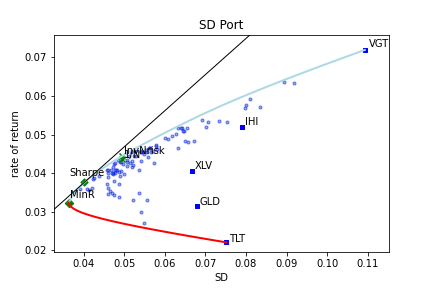
\includegraphics[width=.95\linewidth]{../figs/SDFrontier1.png}
  \caption{Rate of return vs. \SD}
  \label{SD_fig1a}
\end{subfigure}%
\begin{subfigure}{.5\textwidth}
  \centering
  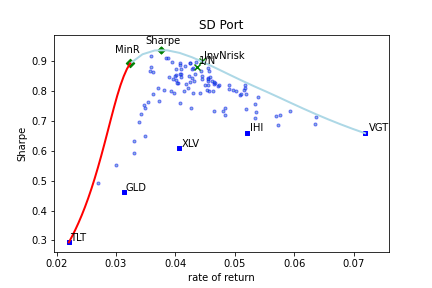
\includegraphics[width=.95\linewidth]{../figs/SDFrontier2.png}
  \caption{Sharpe vs. rate of return}
  \label{SD_fig1b}
\end{subfigure}
\caption{\SD\ frontiers.}
\label{SD_fig1}
\end{figure}

\BackToContents

\subsubsection{Backtesting Sharpe optimal portfolio}

Here is an example, using \azapy\ package, of computing a portfolio backtesting.
For this example, we have chosen a portfolio quarterly rebalanced according
to the maximization of Sharpe ratio. At each rebalancing date,
the portfolio weights
are calibrated based on 3.25 years of prior historical market data.

Other rebalancing strategies can be considered
by changing the value of {\it rtype} parameter in the call of {\it set\_model} function below.
For more details see the package documentation at \azapydoc.

\lstinputlisting[language=Python]{../PyScripts/SD_Port.py}

\begin{figure}[H]
    \centering
    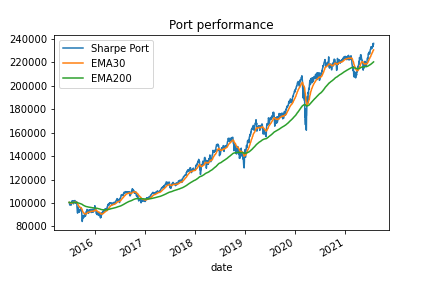
\includegraphics[width=.95\linewidth]{../figs/Port_SD_Sharpe.png}
    \caption{Backtesting of quarterly rebalanced Sharpe optimal portfolio.}
    \label{SD_Port_fig}
\end{figure}

\BackToContents



\subsection{MV-based optimization strategies}\label{S:MV}

\subsubsection{MV dispersion measure}
Variance is the dispersion measure for \MV-based optimal portfolios.
For a portfolio defined by the vector of weights $w$, the variance can
be expressed as
\begin{equation}
    \VAR = w^T \cdot C \cdot w,
    \label{mv00}
\end{equation}
where $C$ is the covariance matrix between the portfolio components.
Alternatively, assuming $C=U^T\cdot U$ factorization, \VAR\ can be rewritten in terms of Euclidian norm as
\begin{equation}
    \VAR = \|U \cdot w\|_2^2.
    \label{mv0}
\end{equation}
We will use both expressions.

\BackToContents

\subsubsection{MV optimal portfolio}
This optimization is described by Eqs.~(\ref{gg1}) from Sec~\ref{strategies} point~\ref{OptRisk},
where $\rho$ is given by \VAR\ from Eq.~(\ref{mv00}).
It is the following QP problem.

\bigskip
\noindent Minimize over $\{ \{w_k\}_{k=1,\cdots,M}, t\}$
\begin{subequations}\label{mv1}
\begin{align}
    & g = \frac{1}{2} w^T C w, \label{mv1a} \\
    \st & \sum_{k=1}^M w_k \mu_k \geq \mu_0, \label{mv1b} \\
        & \sum_{k=1}^M w_k = 1, \label{mv1c} \\
        & w_k \geq 0, \label{mv1d}
\end{align}
\end{subequations}

\noindent where $\mu$, in Eq.~(\ref{mv1b}),
is the targeted portfolio expected rate of return, while $\mu_k$ for $k=1,\cdots,M$
are the portfolio components expected rate of returns.
Then, we have
\begin{subequations}\label{mv2}
\begin{align}
    \RR &= \sum_{k=1}^M w_k^* \mu_k, \label{mv2a} \\
    \VAR &= 2 g^*, \label{mv2b}
\end{align}
\end{subequations}

\noindent where $^*$ denotes the solution of QP problem.
In addition to the optimal portfolio weights $\{w_k^*\}_{k=1,\cdots,M}$ and expected
rate of return $\RR$, the
QP solution provides information about the portfolio \VAR.

The set of equations~(\ref{mv1}) are the most celebrated and the most printed set of equations in the world of portfolio optimizations.
They are at the core of Markowitz pioneer work of portfolio theory \cite{Markowitz} and \cite{Markowitz2}. Up to the customary $1/2$ factor
the solution of Eqs.~(\ref{mv1}) is the same as the solution of Eqs.~(\ref{sd1}). In fact, they illustrate the generic transformation of
a QP into an SOCP problem.

\bigskip
\noindent Here is an example, using the \azapy\ package, of how to compute the \MV\ optimal portfolio.
The \VAR\ time horizon was set to one quarter and the calibration is performed using 3.25 years of
close-adjusted historical prices (default settings).
For more details see the package documentation at \azapydoc.

\lstinputlisting[language=Python]{../PyScripts/MV_RiskOptim.py}

\BackToContents


\subsubsection{Minimum \VAR\ portfolio}

Following the results from Sec.~\ref{strategies} point~\ref{MinRisk},
the algorithm to compute the portfolio with minimum \VAR\ is given by the QP problem from Eqs.~(\ref{mv1}) where
$\mu$ from r.h.s. of Eq.~(\ref{mv1b}) is set to a value equal to the smallest expected rate of
return among the portfolio components, \ie\ $\mu=\min_k\{\mu_k\}$.
Note that minimum \VAR\ and minimum \SD\ portfolios are identical.

\bigskip
\noindent Here is an example, using the \azapy\ package, of how to compute the minimum \VAR\ optimal portfolio.
The \VAR\ time horizon was set to one quarter and the calibration is performed using 3.25 years of
close-adjusted historical prices (default settings).
For more details see the package documentation at \azapydoc.

\lstinputlisting[language=Python]{../PyScripts/MV_MinRisk.py}

\BackToContents


\subsubsection{MV optimal portfolio for targeted risk value}
This optimization is described by Eqs.~(\ref{gg2}) from Sec.~\ref{strategies} point~\ref{TargetRisk},
where $\rho$ given by \VAR\ from Eq.\ (\ref{mv0}).
It is the following SOCP problem.

\bigskip
\noindent Maximize over $\{ w_k \}_{k=1,\cdots, M}$
\begin{subequations}\label{mv3}
\begin{align}
    & g = \sum_{k=1}^M w_k \mu_k, \label{mv3a} \\
    \st & \| U w\|_2 \leq \sqrt{\VAR_0}, \label{mv3b} \\
        & \sum_{k=1}^M w_k = 1, \label{mv3c} \\
        & w_k \geq 0, \label{mv3d}
\end{align}
\end{subequations}

\noindent where $\VAR_0$ from Eq.~(\ref{mv3b}) is the targeted portfolio variance value.
The portfolio expected rate of return is given by the value of the objective
function, \ie,
\begin{equation}
    \RR = g^*, \label{mv4}
\end{equation}

\noindent and the optimal portfolio weights by $\{w^*_k\}_{k=1,\cdots,M}$. The superscript $^*$ denotes the
solution of SOCP problem.

By and large, these sets of equations are a reprint of Eqs.~(\ref{sd3}) and (\ref{sd4}).
Therefore, the \MV\ and \SD\ optimal portfolios with similar targeted risk (\ie\ $\VAR_0 = \SD_0^2$) are identical.

\bigskip
\noindent Here is an example, using the \azapy\ package, of how to compute the optimal portfolio
with the same \VAR\ as the equal weighted portfolio.
The \VAR\ time horizon was set to one quarter and the calibration is performed using 3.25 years of
close-adjusted historical prices (default settings).
For more details see the package documentation at \azapydoc.

\lstinputlisting[language=Python]{../PyScripts/MV_InvNrisk.py}

\BackToContents


\subsubsection{MV optimal portfolio for fixed risk-aversion factor}
This optimization is described by Eqs.~(\ref{gg3}) from Sec.~\ref{strategies} point~\ref{RiskAverse},
where $\rho$ is given by \VAR\ from Eq.\ (\ref{mv00}).
It can be written as the following QP problem.

\bigskip
\noindent Minimize over $\{ w_k \}_{k=1,\cdots,M}$
\begin{subequations}\label{mv5}
\begin{align}
    & g = \frac{1}{2}\left( w^T C w \right) - \frac{1}{2\lambda} \sum_{k=1}^M w_k \mu_k, \label{mv5a} \\
    \st & \sum_{k=1}^M w_k =1, \label{mv5b} \\
        & w_k \geq 0, \label{mv5c}
\end{align}
\end{subequations}

\noindent where $\lambda$ from Eq.\ (\ref{mv5a}) is the risk-aversion factor.
Then, we have
\begin{subequations}\label{mv6}
\begin{align}
    \RR &= \sum_{k=1}^M w_k^* \mu_k, \label{mv6a} \\
    \VAR &= 2 g^* + \frac{\RR}{\lambda}, \label{mv6b}
\end{align}
\end{subequations}

\noindent where $^*$ denotes the solution of QP problem.
In addition to the optimal portfolio weights $\{w_k^*\}_{k=1,\cdots,M}$ and expected rate of return $\RR$, the
QP solution provides information about the portfolio \VAR.

Note that, in this case, the \SD\ and \MV\ optimal portfolio for the same value of $\lambda$ are different.
Both portfolios belong to the \MV\ efficient frontiers (identical with \SD\ efficient frontiers). However, $\lambda$
in the \MV\ representation provides a different parametrization of the efficient frontiers than $\lambda$ in the
\SD\ representation.

\bigskip
\noindent Here is an example, using the \azapy\ package, of how to compute the optimal portfolio
for a given value of the risk-aversion factor $\lambda$.
The \VAR\ time horizon was set to one quarter and the calibration is performed using 3.25 years of
close-adjusted historical prices (default settings).
For more details see the package documentation at \azapydoc.

\lstinputlisting[language=Python]{../PyScripts/MV_Averse.py}

\BackToContents


\subsubsection{\MV-Sharpe optimal portfolio - maximization solution}
This optimization targets the maximization of \MV-Sharpe ratio. It is based on
Eqs.~(\ref{gg4}) from Sec.~\ref{strategies} point~\ref{MaxSharpe},
where $\rho$ is given by \VAR\ from Eq.~(\ref{mv00}).
The optimization can be formulated as an SOCP problem
if Eq.~(\ref{gg4b}) can be expressed as a second order cone constraint.
This can be achieved by
introducing the variable transformations
$\bw_k = t w_k$. Then, the SOCP problem can be written as follows.

\bigskip
\noindent Maximize over $\{ \{ \bw_k\}_{k=1,\cdots,M}, t\}$
\begin{subequations}\label{mv7}
\begin{align}
    & g = \sum_{k=1}^M \bw_k \mu_k - \mu_0 t, \label{mv7a} \\
    \st & \left\| \left(\bw^T \cdot U^T , t - \frac{1}{4} \right)^T \right\|_2 \leq t + \frac{1}{4}, \label{mv7b} \\
        & \sum_{k=1}^M \bw_k - t = 0, \label{mv7c} \\
        & t \geq 0, \label{mv7e} \\
        & w_k \geq 0, \label{mv7d}
\end{align}
\end{subequations}

\noindent where $\mu_0$ from Eq.~(\ref{sd7a}) is the risk-free rate accessible to the investor.

Equation~(\ref{mv7b}) is the Euclidian norm representation of
\begin{equation}
    \bw^T \cdot C \cdot \bw \leq t,
    \label{mv8}
\end{equation}
originated from Eq.~(\ref{gg6b}) after a multiplication by $t$ on both sides. Indeed, it is straightforward to show
that, Eq.~(\ref{mv8}) is equivalent to
\begin{equation}
    \left[ \bw^T C \bw +\left(t - \frac{1}{4}\right)^2 \right]^{1/2} \leq t + \frac{1}{4}.
    \label{mv9}
\end{equation}
The l.h.s. is the Euclidian norm of $\left(\bw^T \cdot U^T , t - \frac{1}{4} \right)^T$ vector, that enters
in Eq.~(\ref{mv7b}).


Then, we have
\begin{subequations}\label{mv10}
\begin{align}
    w_k &= \frac{\bw_k^*}{t^*} , \label{mv10a} \\
    \Sharpe &= g^*, \label{mv10b} \\
    \RR &= \frac{g^*}{t^*} + \mu_0, \label{mv10c} \\
    \VAR &= \frac{1}{t^*}, \label{mv10d}
\end{align}
\end{subequations}

\noindent where $^*$ denotes the solution of SOCP problem.
In addition to the optimal portfolio weights $\{w_k\}_{k=1,\cdots,M}$, expected rate of return $\RR$ and
the \MV-Sharpe ratio $\Sharpe$,
the SOCP solution provides information about the portfolio \VAR.


\bigskip
\noindent Here is an example, using the \azapy\ package, of how to compute the \MV-Sharpe optimal portfolio using the maximization
of \MV-Sharpe ratio.
The \VAR\ time horizon was set to one quarter and the calibration is performed using 3.25 years of
close-adjusted historical prices (default settings).
For more details see the package documentation at \azapydoc.

\lstinputlisting[language=Python]{../PyScripts/MV_Sharpe.py}

\BackToContents

\subsubsection{\MV-Sharpe optimal portfolio - minimization solution}
This optimization targets the minimization of the inverse of \MV-Sharpe ratio.
It is described by Eqs.~(\ref{gg8}) from Sec.~\ref{strategies} point~\ref{MinSharpe}, where
$\rho$ is given by \VAR\ from Eq.~(\ref{mv0}).
The optimization can be formulated as an SOCP problem if Eq.~(\ref{gg8a}) can be expressed as a second order cone constraint. This can be achieved by
introducing a new variable $\eta$ such that
\begin{equation}
    \eta \geq t w^T \cdot C \cdot w,
    \label{mv11}
\end{equation}
and the variable transformations $\bw_k = t w_k$.
Then, the SOCP problem can be written as follows.

\bigskip
\noindent Minimize over $\{ \{ \bw_k\}_{k=1,\cdots,M}, \eta, t\}$
\begin{subequations}\label{mv12}
\begin{align}
    & g = \eta, \label{mv12a} \\
    \st & \left\| \left( \bw^T \cdot U^T , \frac{\eta}{\sqrt{2}} , \frac{t}{\sqrt{2}}  \right)^T \right\|_2
                \leq \frac{\eta}{\sqrt{2}}  + \frac{t}{\sqrt{2}} , \label{mv12b} \\
        & \sum_{k=1}^m \bw_k \mu_k - \mu_0 t = 1, \label{mv12c} \\
        & \sum_{k=1}^M \bw_k - t = 0, \label{mv12d} \\
        &t \geq 0, \label{mv12e} \\
        &\eta \geq 0, \label{mv12f} \\
        &\bw_k \geq 0, \label{mv12g}
 \end{align}
\end{subequations}

\noindent where $\mu_0$ from Eq.~(\ref{mv12c}) is the risk-free rate accessible to the investor.

Equation~(\ref{mv12b}) is the Euclidian norm representation of Eq.~(\ref{mv11}), after
an additional multiplication by $t$ on both sides, \ie,
\begin{equation}
    \bw^T\cdot C\cdot \bw \leq t\eta.
    \label{mv13}
\end{equation}
Indeed, it is straightforward to show that, Eq.~(\ref{mv13}) is equivalent to
\begin{equation}
    \left( \bw^T C \bw + \frac{1}{2}\eta^2 + \frac{1}{2}t^2 \right)^{1/2} \leq \frac{\eta}{\sqrt{2}} + \frac{t}{\sqrt{2}}.
    \label{mv14}
\end{equation}
The l.h.s. is the Euclidian norm of $\left( \bw^T \cdot U^T , \frac{\eta}{\sqrt{2}} , \frac{t}{\sqrt{2}}  \right)^T$ vector, that
enters in Eq.~(\ref{mv12b}).

Then, we have
\begin{subequations}\label{mv15}
\begin{align}
    w_k &= \frac{\bw_k^*}{t^*}, \label{mv15a} \\
    \RR &= \frac{1}{t^*} + \mu_0, \label{mv15c} \\
    \Sharpe &= \frac{1}{g^*}, \label{mv15b} \\
    \VAR &= \frac{g^*}{t^*}, \label{mv15d}
 \end{align}
\end{subequations}

\noindent where $^*$ denotes the solution of SOCP problem.
In addition to the optimal portfolio weights $\{w_k\}_{k=1,\cdots,M}$, expected rate of return $\RR$ and
the \MV-Sharpe ratio $\Sharpe$,
the SOCP solution provides information about the portfolio \VAR.

\bigskip
\noindent Here is an example, using the \azapy\ package, of how to compute the \MV-Sharpe optimal portfolio using the minimization
of the inverse of \MV-Sharpe ratio.
The \VAR\ time horizon was set to one quarter and the calibration is performed using 3.25 years of
close-adjusted historical prices (default settings).
For more details see the package documentation at \azapydoc.

\lstinputlisting[language=Python]{../PyScripts/MV_InvSharpe.py}

\BackToContents


\subsubsection{MV frontiers}

Here is an example of how to compute the \MV\ frontiers using the \azapy\
package. The \VAR\ time horizon was set to one quarter and the calibration is performed using 3.25 years of
close-adjusted historical prices (default settings).
For more details see the package documentation at \azapydoc.

The script produces the plots in Figs. \ref{MV_fig1a} and \ref{MV_fig1b}
for historical data collected up to 2021-07-27.

\lstinputlisting[language=Python]{../PyScripts/MV_frontiers.py}

\begin{figure}[H]
\centering
\begin{subfigure}{.5\textwidth}
  \centering
  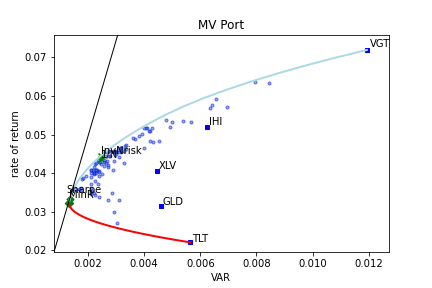
\includegraphics[width=.95\linewidth]{../figs/MVFrontier1.png}
  \caption{Rate of return vs. \VAR}
  \label{MV_fig1a}
\end{subfigure}%
\begin{subfigure}{.5\textwidth}
  \centering
  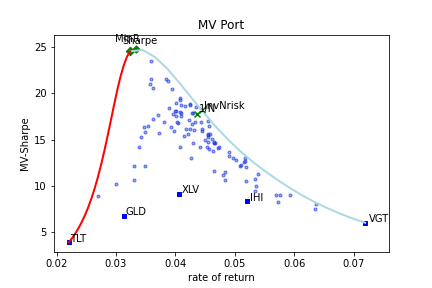
\includegraphics[width=.95\linewidth]{../figs/MVFrontier2.png}
  \caption{\MV-Sharpe vs. rate of return}
  \label{MV_fig1b}
\end{subfigure}
\caption{\MV\ frontiers.}
\label{MV_fig1}
\end{figure}

\BackToContents


\subsubsection{Backtesting MV-Sharpe optimal portfolio}

Here is an example, using \azapy\ package, of computing a portfolio backtesting.
For this example, we have chosen a portfolio quarterly rebalanced according
to the maximization of \MV-Sharpe ratio. At each rebalancing date,
the portfolio weights
are calibrated based on 3.25 years of prior historical market data.

Other rebalancing strategies can be considered
by changing the value of {\it rtype} parameter in the call of {\it set\_model} function below.
For more details see the package documentation at \azapydoc.

\lstinputlisting[language=Python]{../PyScripts/MV_Port.py}

\begin{figure}[H]
    \centering
    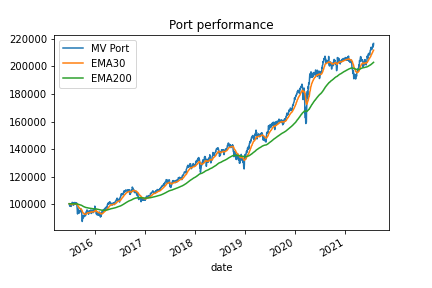
\includegraphics[width=.95\linewidth]{../figs/Port_MV_Sharpe.png}
    \caption{Backtesting of quarterly rebalanced \MV-Sharpe optimal portfolio.}
    \label{MV_Port_fig}
\end{figure}

\BackToContents





\pagebreak
\begin{thebibliography}{99}

\addcontentsline{toc}{section}{References}

\bibitem{Markowitz} Markowitz, H. (1952) "Portfolio selection"
(\href{https://www.math.hkust.edu.hk/~maykwok/courses/ma362/07F/markowitz_JF.pdf}{PDF}), The journal of Finance, 7(1), pp.77-91.

\bibitem{Sharpe1966} Sharpe, W.F. (1966) "Mutual Fund Performance"
(\href{http://www.stat.ucla.edu/~nchristo/statistics_c183_c283/sharpe__mutual_fund_performance.pdf}{PDF}),
The Journal of Business, 39(1), pp.119-138.

\bibitem{MM} Marinescu, M. (2020) "C-Sharpe optimal portfolio"
(\href{https://ssrn.com/abstract=3671774}{PDF}). SSRN July 2020.

\bibitem{Charnes} Charnes, A. and Cooper, W.W. (1962) "Programming with Linear Fractional Functionals",
Naval Research Logistics Quarterly, 9(3–4), pp.181-186.

\bibitem{Acerbi} Acerbi, C. (2002) "Spectral Measures of Risk: A Coherent Representation of Subjective Risk Aversion"
(\href{http://www.pacca.info/public/files/docs/public/finance/Active\%20Risk\%20Management/SpectralMeasures.pdf}{PDF}),
Journal of Banking  Finance, 26(7), pp.1505–1518.

\bibitem{Artzner} Artzner, P., Delbaen, F., Eber, J.-M and Heath, D. (1999) "Coherent measure of risk"
(\href{http://www.planchet.net/EXT/ISFA/1226.nsf/9c8e3fd4d8874d60c1257052003eced6/0bd2345fdff664eec1256e16004ff688/$FILE/Coherent\%20Measures\%20of\%20Risk.pdf}{PDF}),
Mathematical Finance, 9(3), pp.203-228.

\bibitem{Uryasev} Rockafellar, R.T. and Uryasev, S.P. (2000) "Optimization of conditional value-at-risk"
(\href{https://sites.math.washington.edu/~rtr/papers/rtr179-CVaR1.pdf}{PDF}), Journal of Risk, 2(3), pp.21-42.

\bibitem{Pflug} Pflug, G.C. (2000) "Some Remarks on the Value-at-Risk and the Conditional Value-at-Risk"
(\href{http://www.pacca.info/public/files/docs/public/finance/Active\%20Risk\%20Management/gpfl.pdf}{PDF}), In: Uryasev S.P. (edt) "Probabilistic Constrained Optimization.
Nonconvex Optimization and Its Applications", vol 49, Springer, Boston, MA.

\bibitem{Uryasev2} Rockafellar, R.T. and Uryasev, S.P. (2001) "Conditional Value-at-Risk for general loss distributions"
(\href{https://ssrn.com/abstract=267256}{PDF}), SSRN Apri 2001.

\bibitem{Mansini} Mansini, R., Ogryczak, W. and Speranza, M.G. (2014) "Twenty years of linear programming based portfolio optimization"
(\href{http://staff.elka.pw.edu.pl/~wogrycza/publikacje/artykuly/ejor20y.pdf}{PDF}), European Journal of Operational Research, 234, pp.518-535.

\bibitem{Krokhmal} Krokhmal, P.A. (2007) "Higer momentum coherent risk measures"
(\href{http://u.arizona.edu/~krokhmal/pdf/hmcr-qf.pdf}{PDF}), Quantitative Finance, 7, pp.373-387

\bibitem{Ogryczak} Michalowaki, W., and Ogryczak, W. (2001) "Extending the MAD portfolio optimization model to incorporate downside risk aversion"
(\href{https://www.researchgate.net/publication/227653131_Extending_the_MAD_portfolio_optimization_model_to_incorporate_downside_risk_aversion}{PDF}).
Naval Research Logistics, 48 (3), pp.185-200.

\bibitem{Konno} Konno, H., and Yamazaki, H. (1991) "Mean-absolute deviation portfolio optimization model and its application
to Tokyo stock market", Management Science, 37(5), pp.519-531.

\bibitem{Markowitz2} Markowitz, H. (1959), "Portfolio selection"
(\href{https://cowles.yale.edu/sites/default/files/files/pub/mon/m16-all.pdf}{PDF}),  New York, John Wiley and Sons, Inc.

\bibitem{Keating} Keating, C. and Shadwick, F.W. (2002) "A universal performance measure"
(\href{https://www.actuaries.org.uk/system/files/documents/pdf/keating.pdf}{PDF}),
Journal of performance masurament, 6(3), pp.59-84.

\bibitem{Sortino} Sortino, F.A. and Price, L.N. (1994) "Performance measurement in a downside risk framework",
The Journal of Investing, 3(3), pp.59-64.

\bibitem{Kaplan} Kaplan, P.D. and  Knowles, J.A. (2004) "Kappa: A generalized downside risk-adjusted performance measure"
(\href{http://ww.performance-measurement.org/KaplanKnowles2004.pdf}{PDF}),
Journal of Performance Measurement, 8(1), pp.42–54.

\bibitem{Giorgi} Giorgi, G.M. and Gigliarano, C. (2017) "The Gini concentration index: a review of the inference literature"
(\href{https://papers.ssrn.com/sol3/papers.cfm?abstract_id=3016694}{PDF}),
Journal of Economic Survey, 31(4), pp.1130-1148, (availabel at \href{https://papers.ssrn.com/sol3/papers.cfm?abstract_id=3016694}{SSRN}).

\bibitem{Yitzhaki} Yitzhaki, S. (1982) "Stochastic Dominance, Mean Variance, and Gini's Mean Difference"
(\href{https://www.researchgate.net/publication/4900733_Stochastic_Dominance_Mean_Variance_and_Gini's_Mean_Difference}{PDF}),
American Economic Review, 72(1), pp.178-185.

\bibitem{Sharpe1994} Sharpe, W.F. (1994) "The Shapre ratio"
(\href{https://www.earnforex.com/books/en/advanced-forex-trading/The_Sharpe_Ratio.pdf}{PDF}),
Journal of Portfolio Management, 21, pp.49-58.

\bibitem{ecos} Domahidi, A., Chu, E. and Boyd, S. (2013) "ECOS: An SOCP solver for embedded systems".
(\href{https://web.stanford.edu/~boyd/papers/pdf/ecos_ecc.pdf}{PDF}),
European Control Conference (ECC), 2013, pp.3071-3076.

\bibitem{highs-ds} Huangfu, Q.  and Hall, J.A.J. (2018) "Parallelizing the dual revised simplex method"
(\href{https://www.maths.ed.ac.uk/~jajhall/HuHa13/HuHa13.pdf}{PDF}),
Mathematical Programming Computation, 10(1), pp.119-142.






%
%
%
%\bibitem{Krokhmal2} Krokhmal, P.A. and Soberanis, P., (2010) "Risk optimization with p-order cone constraints: A linear programing approach"
%(\href{http://u.arizona.edu/~krokhmal/pdf/hmcr-lp-web.pdf}{PDF}). European Journal of Operational Research 2010 (3): 653-671.
%
%
%\bibitem{Konno2} Konno, H., Waki, H., and Yuuki, A., (2002), "Portfolio optimization under lower partial risk measures"
%(\href{https://www.academia.edu/10202002/Portfolio_optimization_under_lower_partial_risk_measures}{PDF}).
%Asia-Pacific Financial Markets 9: 127-140.
%
%
%\bibitem{Lopez1}  Bailey, D.H., and López de Prado, M.M., (2012), "The Sharpe ratio efficient frontier"
%(\href{https://papers.ssrn.com/sol3/papers.cfm?abstract_id=1821643}{PDF}).
%Journal of Risk 15(2): 3-44.
%
%\bibitem{Roman} Roman, D., and Mitra G., (2009). "Portfolio selection models: A riview and new directions"
%(\href{https://www.academia.edu/9571127/Portfolio_Optimisation_Models_and_Properties_of_Return_Distributions}{PDF}.
%Wilmott Jounal, 1 (2): 69-85.








\end{thebibliography} 
\BackToContents

\pagebreak
\appendix
\addcontentsline{toc}{section}{Appendices}
\section*{Appendices}


\section{azapy package}\label{AZAPY}

\azapy\ is an open-source Python package for portfolio optimizations.
It is released under GNU General Public License v3.0 (GPL-3).
Besides the set of algorithms presented in this paper, \azapy\ implements several other
portfolio strategies. It is a work in progress free for everyone to use and explore.

The package technical documentation is at  \azapydoc\ and its source code at
\azapycode.
It can be installed in a Python environment by calling
\begin{lstlisting}[language=Python]
    pip install azapy
\end{lstlisting}
The \azapy\ development has two major goals:
\begin{itemize}
  \item provide a technical environment to study and compare various portfolio optimizations (in-sample and out-of-sample),
  \item provide an analytic library to support the maintenance of a portfolio rebalancing schedule for a retail type of investor.
\end{itemize}

The library has its own module to collect and maintain historical market data. Several market data providers
are supported. Some of them are free while other require subscriptions.
The list of current supported providers is present in the package documentation at \azapydoc.

The optimization algorithms are using open-source packages for LP, QP and SCOP:
\ecos~\cite{ecos}, \highs~\cite{highs-ds} through \linprog, \cvxopt, and \glpk.

We would like to express our thanks to all developers who were generous to give us unselfish access to their work and imagination.

All the optimization algorithms presented in this paper are accompanied by a simple illustrative Python script.
A set of more complex Python and Jupyter Notebook scripts are present at \azapycode\ under directories {\tt scripts} and {\tt jpy-scripts}, respectively.
The idea is to use them as examples for calling various \azapy\ functionalities as well as sources of inspiration in your work.

If you like to comment or contribute to this project, feel free to contact us (details are at PyPi page \azapy).

\BackToContents 

\section{Portfolio backtesting}\label{backtesting}

Backtesting, also called historical simulation or (recently borrowed from Machine Learning terminology) out-of-sample testing
is the process of testing and measuring the predictive power of an investment strategy using historical data that are not part of the calibration set.

In our case we have built an application to simulate, using historical data, an investment in a portfolio periodically rebalanced according with any of the
optimal strategies mentioned in this paper. The weights are calibrated using a predefined historical period, prior to each of the rebalancing dates.
The actual implementation can be accessed through \azapy\ package. In this paper, several simple Python script examples of backtesting were presented for Sharpe type of optimal
portfolios. They can be easily extended to all other optimization strategies (see the documentation at \azapydoc).

We had in mind a retail investor with limited computational resources and trading execution capabilities.\footnote{In contrast to an
institutional investor with ultra-fast computation and execution capabilities. In this case most of the financial slippages mentioned here can be eliminated.}
The portfolio is rebalanced quarterly, 3 business days before the calendar quarter end. The trading execution is assumed to
be performed at the closing prices.
The portfolio weights are computed after the close of the business day before the
execution day.
We have used the New York Stock Exchange business calendar.
The offset of rebalancing date, the offset of weights calculation date, the length of the historical calibration period,
the length of the entire historical simulation, etc. are parameters that can be adjusted in the \azapy\ implementation, see the documentation at \azapydoc.


In this process there are several assumptions that in real life may lead to cash slippages. Let us list them.
\begin{itemize}
  \item The dividends are assumed to be available for reinvestment on the next rebalancing day after the ex-dividend date.
  In general, there is a delay of a week or more for the cash dividend to be collected. Therefore, it is possible that not all 
  cash dividends will be available for reinvestment on the rebalancing day. However, they will be available for the
  next rebalancing day. This will create a reinvestment slippage that, we believe, is small enough to be
  irrelevant to the overall investment performance.
  \item The delay of one business day between the weights (and the number of shares) calculation and the trading execution. As we mentioned, we
  are considering a realistic rebalancing schedule for a regular retail investor. Therefore, we assume that the new positions
  (\ie\ the number of shares in the portfolio components) were calculated using the closing prices of the business day before the rebalancing day.
  Therefore, there is a price slippage between the computation and the actual trading execution prices.
  In general, the slippage is small, since often a rebalancing consists in readjusting existing positions by selling and buying
  in roughly equal cash amounts. Although small, we keep track of this type of slippage in our investment model by
  readjusting the capital at each rebalancing date. Its impact to the portfolio performance is small. \azapy\ implementation
  offer a facility to view and keep track of these adjustments.
  \item Execution price slippage between the actual trading execution and the closing prices. The model simulation assumes that all
  the rebalancing trades are occurring at the closing prices. In real life, a typical retail investor may execute trades only through manually entered orders.
  Although these orders can be placed in the last minutes of the trading day (say last 15 min) it cannot be assumed that they are executed
  at the closing price of the day. This type of slippage is small enough to have no impact to the overall investment
  performance.\footnote{Although not yet popular, several brokers offer Market-on-Close (MOC) orders for retail investors,
  further reducing this type of  slippage.}
  \item Rounding off to the nearest whole number of shares slippage. The model assumes that the portfolio positions are whole numbers of shares.
  Although some brokers accept fractional orders, at the time when we are drafting this paper, it is not yet a widely available offer.
  Our investment model keeps track of the resulting roundoff cash slippage as an adjustment to the capital on each rebalancing date.
  In general, its impact to the portfolio performance is small.\footnote{Assuming that the share prices are
  small relative to the total invested capital.} \azapy\ implementation
  offer a facility to view and keep track of these adjustments.
  \item We do not consider the impact of transaction costs. These days, all major brokers are waiving the transaction fees under reasonable
  conditions for most of the US equity products (single shares and ETF's). If you are using a broker that is charging
  transactions fees or trading in exotic products with transaction fees (\eg\ leveraged ETF's, etc.)
  or using a margin account with borrowing costs, etc., then you should consider the impact of
  these fees.
\end{itemize}

\BackToContents


\section{CVaR LP analytical solution}\label{AppendixA}

This appendix presents the proof of statement from Eqs.~(\ref{cvar3}).

It is straightforward to show that,
for $u \in (-x_{k+1}, -x_k]$ the objective function from Eq.~(\ref{cvar1:1})
is given by
\begin{equation}
    g(u) = \frac{a-k}{a} u - \frac{1}{a} \sum_{i=1}^k x_i,
    \label{a:cavr1}
\end{equation}
where $a=(1-\alpha)N$. Thus, $g(u)$ it is a continuous piecewise linear function in $u$. Therefore,
its minimum occurs in one of the vertices $g_k= g(-x_k)$.

We need to find $k^* \in \{1,\cdots,N\}$  such that $g_{k^*}$ has the smallest value.

After simple algebraic manipulations, we can write
\begin{equation}
    g_{k+1} - g_{k} = \frac{k - a}{a} (x_{k+1} - x_{k}).
    \label{apx:cvar:1}
\end{equation}
It follows\footnote{Recall that $\{x_i\}$ is $\{r_i\}$ sorted in ascending order. Therefore, $x_{k+1} - x_{k}$ is positive.}
that, if $g_k \leq g_{k+1}$ then $k \geq a$.
Similar, we have
\begin{equation}
    g_{k} - g_{k-1} = \frac{k - 1 - a}{a} (x_{k} - x_{k-1}),
\end{equation}
and if $g_k \leq g_{k-1}$ then $k \leq a + 1$.
Therefore, $k^*$ is the integer value between $a$ and $a+1$.
That is $k^* = \lceil a \rceil$. Also from Eq.~(\ref{apx:cvar:1}) it is clear that this minimum is unique.
The rest follows.

\BackToContents





\end{document}
